% ---------------------------------------------------------------------------
% Hauptteil, Teil 4: Ergebnisse
%
% Eingebundene Exponate:
%   Abbildung 1  figures/fig01_both_panels.png   (Vektor-Master: gleichnamige .svg)
%   Tabelle  1   tables/tab01_sample_selection   (enthaelt zwei Tabellen:
%                Selektionskette + Abgleich mit den publizierten Werten)
%   Tabelle  2   tables/tab02_descriptives
%   Tabelle  3   tables/tab03_employment
%   Tabelle  4   tables/tab04_intermediate_outcomes  (enthaelt zwei Tabellen:
%                Panels A--D + Abgleich mit den publizierten Werten)
%   Abbildung 2  figures/fig02_all_panels.png   (Vektor-Master: gleichnamige .svg;
%                Einzelpanels liegen als fig02_panel_{a,b,c} daneben)
%   Tabelle  5   tables/tab05_mediation  (enthaelt zwei Tabellen: Modelle 1.3--1.8
%                + Abgleich mit den publizierten Werten)
% ---------------------------------------------------------------------------

\chapter{Ergebnisse}
\label{cha:ergebnisse}

Die Darstellung der Befunde folgt dem Aufbau der Replikation: zun\"achst die
regionale Variation des Kursangebots, die die Identifikationsstrategie tr\"agt
(Abschnitt~\ref{sec:erg-angebot}), anschlie{\ss}end die Konstruktion der
Analysestichprobe und die deskriptiven Kennwerte
(Abschnitt~\ref{sec:erg-deskriptiv}), anschlie{\ss}end die multivariaten
Sch\"atzungen zur Erwerbsbeteiligung (Abschnitt~\ref{sec:erg-multivariat}) und
schlie{\ss}lich die Frage, \"uber welche Zwischenschritte der Angebotseffekt
zustande kommt \textendash{} zun\"achst mit den intermedi\"aren Ergebnissen als
abh\"angigen Variablen (Abschnitt~\ref{sec:erg-mechanismen}), danach mit
denselben Gr\"o{\ss}en als Kontrollvariablen im Erwerbsmodell
(Abschnitt~\ref{sec:erg-mediation}).


\section{Reproduzierte Ergebnisse}



\subsection{Deskriptive Befunde}
\label{sec:erg-deskriptiv}


Die zweite reproduzierte Tabelle liefert Informationen zu den deskriptiven Statistiken der in den empirischen Analysen verwendeten Modellvariablen. Zusammen mit dieser Tabelle ermöglicht sie es, Einblicke sowohl in die zentralen Variablen der Untersuchung als auch in die Verteilung aller verwendeten Modellvariablen zu gewinnen. In der Tabelle werden Mittelwerte, Standardabweichungen, die Anzahl der Beobachtungen und der jeweilige Wertebereich dargestellt.

Die erste der zentralen Variablen ist die Beschäftigung, die in der Analyse als abhängige Variable verwendet wird. Die Beschäftigung wird in Tabelle 2 als „bezahlte Arbeit“ bezeichnet. Zum Zeitpunkt der Befragung waren 18\% der Befragten in einer bezahlten Beschäftigung tätig.

% GENERATED BY src/python/lmi/tables/tab02_descriptives.py -- DO NOT EDIT
%==============================================================================%
% tab02_descriptives.tex
%
% Purpose : Tabelle 2 der Replikation -- unstandardisierte deskriptive
%           Statistiken der Modellvariablen. Entspricht Table 2 in Kanas &
%           Kosyakova, S. 16 (Bib-Key: Kanas:2023).
% Source  : SOEPremote job 244565, src/stata/remote/descriptives_micro.do
%           Rohlisting: results/transcripts/src_stata_remote_descriptives_micro.do.eml
%           Transkript: results/comparisons/tab02_descriptives.md
% Needs   : booktabs, tabularx (beide bereits in bachelorarbeit.sty geladen)
% Usage   : % GENERATED BY src/python/lmi/tables/tab02_descriptives.py -- DO NOT EDIT
%==============================================================================%
% tab02_descriptives.tex
%
% Purpose : Tabelle 2 der Replikation -- unstandardisierte deskriptive
%           Statistiken der Modellvariablen. Entspricht Table 2 in Kanas &
%           Kosyakova, S. 16 (Bib-Key: Kanas:2023).
% Source  : SOEPremote job 244565, src/stata/remote/descriptives_micro.do
%           Rohlisting: results/transcripts/src_stata_remote_descriptives_micro.do.eml
%           Transkript: results/comparisons/tab02_descriptives.md
% Needs   : booktabs, tabularx (beide bereits in bachelorarbeit.sty geladen)
% Usage   : % GENERATED BY src/python/lmi/tables/tab02_descriptives.py -- DO NOT EDIT
%==============================================================================%
% tab02_descriptives.tex
%
% Purpose : Tabelle 2 der Replikation -- unstandardisierte deskriptive
%           Statistiken der Modellvariablen. Entspricht Table 2 in Kanas &
%           Kosyakova, S. 16 (Bib-Key: Kanas:2023).
% Source  : SOEPremote job 244565, src/stata/remote/descriptives_micro.do
%           Rohlisting: results/transcripts/src_stata_remote_descriptives_micro.do.eml
%           Transkript: results/comparisons/tab02_descriptives.md
% Needs   : booktabs, tabularx (beide bereits in bachelorarbeit.sty geladen)
% Usage   : \input{tables/tab02_descriptives}
% Author  : Emre Suemer, 2026-08-13
%==============================================================================%

\makeatletter
\@ifundefined{NC@rewrite@Z}{%
  \newcolumntype{Z}{>{\raggedright\arraybackslash\hangindent=1.9em\hangafter=1}X}%
}{}
\makeatother

\begin{table}[htbp]
  \centering
  \caption{Unstandardisierte deskriptive Statistiken der Modellvariablen}
  \label{tab:deskriptiv}
  \footnotesize
  \setlength{\tabcolsep}{4pt}%
  \begin{tabularx}{\textwidth}{@{}Zrrr@{}}
    \toprule
    Variable & Mittelwert/Anteil (SD) & N & Wertebereich \\
    \midrule
    In bezahlter Arbeit & 0{,}18 & 5.467 & 0/1 \\
    Deutsche Sprachkenntnisse & 5{,}40 (2{,}95) & 5.463 & 0--12 \\
    Integrationskurs abgeschlossen & 0{,}29 & 5.197 & 0/1 \\
    Sprachzertifikat erworben & 0{,}43 & 5.455 & 0/1 \\
    H\"aufigkeit des Kontakts zu Deutschen & 2{,}73 (1{,}89) & 5.449 & 0--5 \\
    \textbf{Kreisangebot an Integrationskursen, std.} & 0{,}00 (1{,}00) & 5.467 & $-$1{,}57--5{,}18 \\
    Aufenthaltsdauer, in Monaten (/12) & 2{,}42 (1{,}13) & 5.467 & 0{,}00--5{,}83 \\
    Bildungsjahre vor der Migration & 8{,}98 (5{,}25) & 5.129 & 0--27 \\
    Erwerbserfahrung vor der Migration & 0{,}64 & 5.224 & 0/1 \\
    Weiblich & 0{,}37 & 5.467 & 0/1 \\
    Kinder unter 16 Jahren im Haushalt & 0{,}63 & 5.462 & 0/1 \\
    Einreise mit der Familie & 0{,}34 & 5.467 & 0/1 \\
    Unterst\"utzung durch Familie/Verwandte in DE & 0{,}14 & 5.440 & 0/1 \\
    Alter bei der Erstbefragung & 31{,}74 (9{,}81) & 5.467 & 18--64 \\
    Traumatische Erfahrungen & 0{,}56 & 3.492 & 0/1 \\
    Status des Asylantrags &  & 5.467 &  \\
    \quad -- Keine Entscheidung & 0{,}39 &  & 0/1 \\
    \quad -- Anerkannt & 0{,}38 &  & 0/1 \\
    \quad -- Abgelehnt & 0{,}23 &  & 0/1 \\
    Kreisanteil Ausl\"ander:innen, std. & 0{,}00 (1{,}00) & 5.467 & $-$1{,}82--2{,}99 \\
    Kreisbev\"olkerungsdichte, std. & 0{,}00 (1{,}00) & 5.467 & $-$0{,}86--2{,}73 \\
    Kreisarbeitslosenquote, std. & 0{,}00 (1{,}00) & 5.467 & $-$1{,}86--3{,}04 \\
    Kreissorgen \"uber Zuwanderung, std. & 0{,}00 (1{,}00) & 5.467 & $-$1{,}91--4{,}25 \\
    Kreisanteil CDU/CSU-W\"ahler:innen, std. & 0{,}00 (1{,}00) & 5.467 & $-$2{,}23--2{,}87 \\
    Erhebungsstichprobe &  & 5.467 &  \\
    \quad -- M3 & 0{,}32 &  & 0/1 \\
    \quad -- M4 & 0{,}34 &  & 0/1 \\
    \quad -- M5 & 0{,}33 &  & 0/1 \\
    Herkunftsland &  & 5.467 &  \\
    \quad -- Syrien & 0{,}35 &  & 0/1 \\
    \quad -- Afghanistan & 0{,}20 &  & 0/1 \\
    \quad -- Irak & 0{,}17 &  & 0/1 \\
    \quad -- Eritrea & 0{,}05 &  & 0/1 \\
    \quad -- Iran & 0{,}02 &  & 0/1 \\
    \quad -- \"Ubriger Nahost/Nordafrika & 0{,}02 &  & 0/1 \\
    \quad -- Ehemalige UdSSR & 0{,}04 &  & 0/1 \\
    \quad -- Westbalkan & 0{,}04 &  & 0/1 \\
    \quad -- \"Ubriges Afrika & 0{,}07 &  & 0/1 \\
    \quad -- Sonstige & 0{,}04 &  & 0/1 \\
    Erhebungsjahr &  & 5.467 &  \\
    \quad -- 2016 & 0{,}29 &  & 0/1 \\
    \quad -- 2017 & 0{,}33 &  & 0/1 \\
    \quad -- 2018 & 0{,}23 &  & 0/1 \\
    \quad -- 2019 & 0{,}15 &  & 0/1 \\
    \bottomrule
  \end{tabularx}

  \vspace{0.75ex}
  \parbox{\textwidth}{\footnotesize
    \textit{Anmerkungen:} Eigene Berechnung, IAB-BAMF-SOEP-Befragung von
    Gefl\"uchteten 2016--2019, SOEP-Core v36 (Remote Edition), Analysestichprobe
    (5.467 Personenjahre, 2.730 Personen; vgl.
    Tabelle~\ref{tab:stichprobenselektion}). SD = Standardabweichung;
    std.\ = standardisiert. Die schwankenden Fallzahlen spiegeln
    variablenspezifische Item-Nonresponse wider; die Statistiken werden vor der
    multiplen Imputation berechnet (\texttt{mi extract 0}), also
    vollst\"andige-F\"alle-basiert. S\"amtliche 102 in
    \textcite[16]{Kanas:2023} publizierten Werte werden exakt reproduziert
    (40 Mittelwerte, 40 Fallzahlen, 11 Standardabweichungen, 11 Wertebereiche).
    \\[0.4ex]
    \textbf{Abweichung:} Die drei Kategorien des Asylstatus sind
    in der publizierten Tabelle um eine Position rotiert beschriftet
    (dort \glqq Approved 0,39 / Rejected 0,38 / No decision 0,23\grqq).
    Ma\ss{}geblich sind die Wertelabels des Originalcodes
    (\texttt{00013\_data\_clean.do:1541}), wonach Kategorie~1
    \emph{keine Entscheidung} ist. Die Zahlen sind identisch, die Zuordnung oben
    ist die korrigierte.}
\end{table}

% Author  : Emre Suemer, 2026-08-13
%==============================================================================%

\makeatletter
\@ifundefined{NC@rewrite@Z}{%
  \newcolumntype{Z}{>{\raggedright\arraybackslash\hangindent=1.9em\hangafter=1}X}%
}{}
\makeatother

\begin{table}[htbp]
  \centering
  \caption{Unstandardisierte deskriptive Statistiken der Modellvariablen}
  \label{tab:deskriptiv}
  \footnotesize
  \setlength{\tabcolsep}{4pt}%
  \begin{tabularx}{\textwidth}{@{}Zrrr@{}}
    \toprule
    Variable & Mittelwert/Anteil (SD) & N & Wertebereich \\
    \midrule
    In bezahlter Arbeit & 0{,}18 & 5.467 & 0/1 \\
    Deutsche Sprachkenntnisse & 5{,}40 (2{,}95) & 5.463 & 0--12 \\
    Integrationskurs abgeschlossen & 0{,}29 & 5.197 & 0/1 \\
    Sprachzertifikat erworben & 0{,}43 & 5.455 & 0/1 \\
    H\"aufigkeit des Kontakts zu Deutschen & 2{,}73 (1{,}89) & 5.449 & 0--5 \\
    \textbf{Kreisangebot an Integrationskursen, std.} & 0{,}00 (1{,}00) & 5.467 & $-$1{,}57--5{,}18 \\
    Aufenthaltsdauer, in Monaten (/12) & 2{,}42 (1{,}13) & 5.467 & 0{,}00--5{,}83 \\
    Bildungsjahre vor der Migration & 8{,}98 (5{,}25) & 5.129 & 0--27 \\
    Erwerbserfahrung vor der Migration & 0{,}64 & 5.224 & 0/1 \\
    Weiblich & 0{,}37 & 5.467 & 0/1 \\
    Kinder unter 16 Jahren im Haushalt & 0{,}63 & 5.462 & 0/1 \\
    Einreise mit der Familie & 0{,}34 & 5.467 & 0/1 \\
    Unterst\"utzung durch Familie/Verwandte in DE & 0{,}14 & 5.440 & 0/1 \\
    Alter bei der Erstbefragung & 31{,}74 (9{,}81) & 5.467 & 18--64 \\
    Traumatische Erfahrungen & 0{,}56 & 3.492 & 0/1 \\
    Status des Asylantrags &  & 5.467 &  \\
    \quad -- Keine Entscheidung & 0{,}39 &  & 0/1 \\
    \quad -- Anerkannt & 0{,}38 &  & 0/1 \\
    \quad -- Abgelehnt & 0{,}23 &  & 0/1 \\
    Kreisanteil Ausl\"ander:innen, std. & 0{,}00 (1{,}00) & 5.467 & $-$1{,}82--2{,}99 \\
    Kreisbev\"olkerungsdichte, std. & 0{,}00 (1{,}00) & 5.467 & $-$0{,}86--2{,}73 \\
    Kreisarbeitslosenquote, std. & 0{,}00 (1{,}00) & 5.467 & $-$1{,}86--3{,}04 \\
    Kreissorgen \"uber Zuwanderung, std. & 0{,}00 (1{,}00) & 5.467 & $-$1{,}91--4{,}25 \\
    Kreisanteil CDU/CSU-W\"ahler:innen, std. & 0{,}00 (1{,}00) & 5.467 & $-$2{,}23--2{,}87 \\
    Erhebungsstichprobe &  & 5.467 &  \\
    \quad -- M3 & 0{,}32 &  & 0/1 \\
    \quad -- M4 & 0{,}34 &  & 0/1 \\
    \quad -- M5 & 0{,}33 &  & 0/1 \\
    Herkunftsland &  & 5.467 &  \\
    \quad -- Syrien & 0{,}35 &  & 0/1 \\
    \quad -- Afghanistan & 0{,}20 &  & 0/1 \\
    \quad -- Irak & 0{,}17 &  & 0/1 \\
    \quad -- Eritrea & 0{,}05 &  & 0/1 \\
    \quad -- Iran & 0{,}02 &  & 0/1 \\
    \quad -- \"Ubriger Nahost/Nordafrika & 0{,}02 &  & 0/1 \\
    \quad -- Ehemalige UdSSR & 0{,}04 &  & 0/1 \\
    \quad -- Westbalkan & 0{,}04 &  & 0/1 \\
    \quad -- \"Ubriges Afrika & 0{,}07 &  & 0/1 \\
    \quad -- Sonstige & 0{,}04 &  & 0/1 \\
    Erhebungsjahr &  & 5.467 &  \\
    \quad -- 2016 & 0{,}29 &  & 0/1 \\
    \quad -- 2017 & 0{,}33 &  & 0/1 \\
    \quad -- 2018 & 0{,}23 &  & 0/1 \\
    \quad -- 2019 & 0{,}15 &  & 0/1 \\
    \bottomrule
  \end{tabularx}

  \vspace{0.75ex}
  \parbox{\textwidth}{\footnotesize
    \textit{Anmerkungen:} Eigene Berechnung, IAB-BAMF-SOEP-Befragung von
    Gefl\"uchteten 2016--2019, SOEP-Core v36 (Remote Edition), Analysestichprobe
    (5.467 Personenjahre, 2.730 Personen; vgl.
    Tabelle~\ref{tab:stichprobenselektion}). SD = Standardabweichung;
    std.\ = standardisiert. Die schwankenden Fallzahlen spiegeln
    variablenspezifische Item-Nonresponse wider; die Statistiken werden vor der
    multiplen Imputation berechnet (\texttt{mi extract 0}), also
    vollst\"andige-F\"alle-basiert. S\"amtliche 102 in
    \textcite[16]{Kanas:2023} publizierten Werte werden exakt reproduziert
    (40 Mittelwerte, 40 Fallzahlen, 11 Standardabweichungen, 11 Wertebereiche).
    \\[0.4ex]
    \textbf{Abweichung:} Die drei Kategorien des Asylstatus sind
    in der publizierten Tabelle um eine Position rotiert beschriftet
    (dort \glqq Approved 0,39 / Rejected 0,38 / No decision 0,23\grqq).
    Ma\ss{}geblich sind die Wertelabels des Originalcodes
    (\texttt{00013\_data\_clean.do:1541}), wonach Kategorie~1
    \emph{keine Entscheidung} ist. Die Zahlen sind identisch, die Zuordnung oben
    ist die korrigierte.}
\end{table}

% Author  : Emre Suemer, 2026-08-13
%==============================================================================%

\makeatletter
\@ifundefined{NC@rewrite@Z}{%
  \newcolumntype{Z}{>{\raggedright\arraybackslash\hangindent=1.9em\hangafter=1}X}%
}{}
\makeatother

\begin{table}[htbp]
  \centering
  \caption{Unstandardisierte deskriptive Statistiken der Modellvariablen}
  \label{tab:deskriptiv}
  \footnotesize
  \setlength{\tabcolsep}{4pt}%
  \begin{tabularx}{\textwidth}{@{}Zrrr@{}}
    \toprule
    Variable & Mittelwert/Anteil (SD) & N & Wertebereich \\
    \midrule
    In bezahlter Arbeit & 0{,}18 & 5.467 & 0/1 \\
    Deutsche Sprachkenntnisse & 5{,}40 (2{,}95) & 5.463 & 0--12 \\
    Integrationskurs abgeschlossen & 0{,}29 & 5.197 & 0/1 \\
    Sprachzertifikat erworben & 0{,}43 & 5.455 & 0/1 \\
    H\"aufigkeit des Kontakts zu Deutschen & 2{,}73 (1{,}89) & 5.449 & 0--5 \\
    \textbf{Kreisangebot an Integrationskursen, std.} & 0{,}00 (1{,}00) & 5.467 & $-$1{,}57--5{,}18 \\
    Aufenthaltsdauer, in Monaten (/12) & 2{,}42 (1{,}13) & 5.467 & 0{,}00--5{,}83 \\
    Bildungsjahre vor der Migration & 8{,}98 (5{,}25) & 5.129 & 0--27 \\
    Erwerbserfahrung vor der Migration & 0{,}64 & 5.224 & 0/1 \\
    Weiblich & 0{,}37 & 5.467 & 0/1 \\
    Kinder unter 16 Jahren im Haushalt & 0{,}63 & 5.462 & 0/1 \\
    Einreise mit der Familie & 0{,}34 & 5.467 & 0/1 \\
    Unterst\"utzung durch Familie/Verwandte in DE & 0{,}14 & 5.440 & 0/1 \\
    Alter bei der Erstbefragung & 31{,}74 (9{,}81) & 5.467 & 18--64 \\
    Traumatische Erfahrungen & 0{,}56 & 3.492 & 0/1 \\
    Status des Asylantrags &  & 5.467 &  \\
    \quad -- Keine Entscheidung & 0{,}39 &  & 0/1 \\
    \quad -- Anerkannt & 0{,}38 &  & 0/1 \\
    \quad -- Abgelehnt & 0{,}23 &  & 0/1 \\
    Kreisanteil Ausl\"ander:innen, std. & 0{,}00 (1{,}00) & 5.467 & $-$1{,}82--2{,}99 \\
    Kreisbev\"olkerungsdichte, std. & 0{,}00 (1{,}00) & 5.467 & $-$0{,}86--2{,}73 \\
    Kreisarbeitslosenquote, std. & 0{,}00 (1{,}00) & 5.467 & $-$1{,}86--3{,}04 \\
    Kreissorgen \"uber Zuwanderung, std. & 0{,}00 (1{,}00) & 5.467 & $-$1{,}91--4{,}25 \\
    Kreisanteil CDU/CSU-W\"ahler:innen, std. & 0{,}00 (1{,}00) & 5.467 & $-$2{,}23--2{,}87 \\
    Erhebungsstichprobe &  & 5.467 &  \\
    \quad -- M3 & 0{,}32 &  & 0/1 \\
    \quad -- M4 & 0{,}34 &  & 0/1 \\
    \quad -- M5 & 0{,}33 &  & 0/1 \\
    Herkunftsland &  & 5.467 &  \\
    \quad -- Syrien & 0{,}35 &  & 0/1 \\
    \quad -- Afghanistan & 0{,}20 &  & 0/1 \\
    \quad -- Irak & 0{,}17 &  & 0/1 \\
    \quad -- Eritrea & 0{,}05 &  & 0/1 \\
    \quad -- Iran & 0{,}02 &  & 0/1 \\
    \quad -- \"Ubriger Nahost/Nordafrika & 0{,}02 &  & 0/1 \\
    \quad -- Ehemalige UdSSR & 0{,}04 &  & 0/1 \\
    \quad -- Westbalkan & 0{,}04 &  & 0/1 \\
    \quad -- \"Ubriges Afrika & 0{,}07 &  & 0/1 \\
    \quad -- Sonstige & 0{,}04 &  & 0/1 \\
    Erhebungsjahr &  & 5.467 &  \\
    \quad -- 2016 & 0{,}29 &  & 0/1 \\
    \quad -- 2017 & 0{,}33 &  & 0/1 \\
    \quad -- 2018 & 0{,}23 &  & 0/1 \\
    \quad -- 2019 & 0{,}15 &  & 0/1 \\
    \bottomrule
  \end{tabularx}

  \vspace{0.75ex}
  \parbox{\textwidth}{\footnotesize
    \textit{Anmerkungen:} Eigene Berechnung, IAB-BAMF-SOEP-Befragung von
    Gefl\"uchteten 2016--2019, SOEP-Core v36 (Remote Edition), Analysestichprobe
    (5.467 Personenjahre, 2.730 Personen; vgl.
    Tabelle~\ref{tab:stichprobenselektion}). SD = Standardabweichung;
    std.\ = standardisiert. Die schwankenden Fallzahlen spiegeln
    variablenspezifische Item-Nonresponse wider; die Statistiken werden vor der
    multiplen Imputation berechnet (\texttt{mi extract 0}), also
    vollst\"andige-F\"alle-basiert. S\"amtliche 102 in
    \textcite[16]{Kanas:2023} publizierten Werte werden exakt reproduziert
    (40 Mittelwerte, 40 Fallzahlen, 11 Standardabweichungen, 11 Wertebereiche).
    \\[0.4ex]
    \textbf{Abweichung:} Die drei Kategorien des Asylstatus sind
    in der publizierten Tabelle um eine Position rotiert beschriftet
    (dort \glqq Approved 0,39 / Rejected 0,38 / No decision 0,23\grqq).
    Ma\ss{}geblich sind die Wertelabels des Originalcodes
    (\texttt{00013\_data\_clean.do:1541}), wonach Kategorie~1
    \emph{keine Entscheidung} ist. Die Zahlen sind identisch, die Zuordnung oben
    ist die korrigierte.}
\end{table}


Die Verteilung der verschiedenen Variablen zum Thema Integration wird aufgezeigt. Für die Deutschkenntnisse wurde ein Index im Bereich von 0 bis 12 erstellt. Ein Wert von 5,40 Punkten bei den Deutschkenntnissen entspricht in etwa einem mittleren Sprachniveau der Befragten. 29\% der befragten Personen haben einen Integrationskurs abgeschlossen. Der Anteil der Personen, die ein deutsches Sprachzertifikat erworben haben, beträgt 43\%. Die Tabelle zeigt, dass die durchschnittliche Häufigkeit der Kontakte zu Deutschen bei 2,73 liegt; der Wertebereich dieser Variablen wurde auf 0 bis 5 festgelegt.

Als zentrale unabhängige Variable wurde das Angebot an Integrationskursen nach Landkreisen verwendet. Die unabhängige Variable wurde standardisiert, daher beträgt ihr Mittelwert 0,00 und ihre Standardabweichung 1,00. Tabelle 2 zeigt, dass die Werte zwischen -1,57 und 5,18 variieren. Demnach gibt es auf lokaler Ebene Unterschiede im Angebot an Integrationskursen.

Im Gesamtprofil der Stichprobe werden die Verteilungen von Variablen wie Aufenthaltsdauer, Alter und Berufserfahrung vor der Migration dargestellt. Die Aufenthaltsdauer der Geflüchteten in der Stichprobe beträgt im Durchschnitt 2,42 Jahre. 37\% der befragten Geflüchteten sind Frauen, und 63\% haben ein Kind unter 16 Jahren. Der Anteil der Personen mit Berufserfahrung vor der Migration liegt bei 64\%, während die durchschnittliche Schulbesuchsdauer vor der Migration bei 8,98 Jahren liegt.

Tabelle 2 zeigt zudem die Verteilung der Geflüchteten nach ihrem Asylstatus. Bei 39\% der Geflüchteten wurde der Asylantrag positiv beschlossen, während bei 38\% der Geflüchteten der Asylantrag abgelehnt wurde. Der Anteil der Geflüchteten, über deren Asylantrag noch keine Entscheidung getroffen wurde, beträgt 23\%.

Die Kontrollvariablen auf Kreisebene – Anteil der ausländischen Bevölkerung, Bevölkerungsdichte, Arbeitslosenquote, Sorge um die Zuwanderung und CDU/CSU-Anteil – wurden standardisiert und sind in der Tabelle aufgeführt.


\subsection{Multivariate Ergebnisse}
\label{sec:erg-multivariat}

Tabelle 3 zeigt den Zusammenhang zwischen dem Angebot an Integrationskursen in der Region und der bezahlten Beschäftigung. Modell 1.2 verdeutlicht, ob sich dieser Zusammenhang in Abhängigkeit von der Aufenthaltsdauer in Deutschland unterscheidet.

In Modell 1.1 wird gezeigt, dass der Koeffizient für das Kursangebot positiv und statistisch signifikant ist. Es zeigt sich, dass ein Anstieg des Kursangebots um eine Standardabweichung die Beschäftigungswahrscheinlichkeit von Geflüchteten um 2.98 prozentpunkte erhöht. Dies deutet darauf hin, dass ein höheres lokales Kursangebot mit besseren Beschäftigungsaussichten verbunden ist.

Das zweite Ergebnis ist, dass der Interaktionskoeffizient zwischen dem Angebot an Sprachkursen vor Ort und der Aufenthaltsdauer von Geflüchteten in Deutschland bei 0,81 liegt und somit positiv ist. Kanas und Kosyakova (2023) haben festgestellt, dass dieser Wert statistisch nicht signifikant ist (p = 0,282). Es gibt keine Hinweise darauf, dass der Beschäftigungsvorteil von Geflüchteten, die anfangs einem größeren lokalen Angebot an Integrationskursen ausgesetzt waren, von der Dauer ihres Aufenthalts in Deutschland abhängt.

Im Rahmen zusätzlicher Analysen haben Kanas und Kosyakova (2023) getestet, ob sich der Zusammenhang des Kursangebots auf die Beschäftigung je nach verschiedenen Personen- und Kreismerkmalen unterscheiden. Die Ergebnisse sind in Tabelle S6 im Zusatzmaterial zu finden. Es zeigt sich, dass der positive Zusammenhang des lokalen Kursangebots bei Personen mit Berufserfahrung vor der Migration geringer ausfällt. Kanas und Kosyakova (2023) begründen diesen Befund damit, dass geflüchtete Personen mit Berufserfahrung Programme zur Beschäftigungsförderung benötigen, wie beispielsweise berufsspezifische Sprachkurse, verstärkte Berufsberatung und die Vermittlung in Weiterbildungskurse. Ein zweiter Unterschied besteht darin, dass der Zusammenhang zwischen dem Kursangebot und der Beschäftigung in Landkreisen, in denen größere Sorgen hinsichtlich der Zuwanderung bestehen, stärker ausgeprägt ist. Als möglicher Grund dafür wird angeführt, dass die Motivation von Geflüchteten, die in zuwanderungskritischen Landkreisen leben, zum Sprachenlernen und zur Integration in die Aufnahmegesellschaft größer sein könnte.


% GENERATED BY src/python/lmi/tables/tab03_employment.py -- DO NOT EDIT
%==============================================================================%
% tab03_employment.tex
%
% Purpose : Tabelle 3 der Replikation -- Wahrscheinlichkeit bezahlter Arbeit,
%           durchschnittliche marginale Effekte in Prozentpunkten. Entspricht
%           Table 3 in Kanas & Kosyakova, S. 20 (Bib-Key: Kanas:2023).
% Source  : SOEPremote job 244566, src/stata/remote/tab03_employment.do
%           Rohlisting: results/transcripts/src_stata_remote_tab03_employment.do.eml
%           Transkript: results/comparisons/tab03_employment.md
% Needs   : booktabs, tabularx (beide bereits in bachelorarbeit.sty geladen)
% Usage   : % GENERATED BY src/python/lmi/tables/tab03_employment.py -- DO NOT EDIT
%==============================================================================%
% tab03_employment.tex
%
% Purpose : Tabelle 3 der Replikation -- Wahrscheinlichkeit bezahlter Arbeit,
%           durchschnittliche marginale Effekte in Prozentpunkten. Entspricht
%           Table 3 in Kanas & Kosyakova, S. 20 (Bib-Key: Kanas:2023).
% Source  : SOEPremote job 244566, src/stata/remote/tab03_employment.do
%           Rohlisting: results/transcripts/src_stata_remote_tab03_employment.do.eml
%           Transkript: results/comparisons/tab03_employment.md
% Needs   : booktabs, tabularx (beide bereits in bachelorarbeit.sty geladen)
% Usage   : % GENERATED BY src/python/lmi/tables/tab03_employment.py -- DO NOT EDIT
%==============================================================================%
% tab03_employment.tex
%
% Purpose : Tabelle 3 der Replikation -- Wahrscheinlichkeit bezahlter Arbeit,
%           durchschnittliche marginale Effekte in Prozentpunkten. Entspricht
%           Table 3 in Kanas & Kosyakova, S. 20 (Bib-Key: Kanas:2023).
% Source  : SOEPremote job 244566, src/stata/remote/tab03_employment.do
%           Rohlisting: results/transcripts/src_stata_remote_tab03_employment.do.eml
%           Transkript: results/comparisons/tab03_employment.md
% Needs   : booktabs, tabularx (beide bereits in bachelorarbeit.sty geladen)
% Usage   : \input{tables/tab03_employment}
% Author  : Emre Suemer, 2026-08-13
%==============================================================================%

\makeatletter
\@ifundefined{NC@rewrite@Z}{%
  \newcolumntype{Z}{>{\raggedright\arraybackslash\hangindent=1.9em\hangafter=1}X}%
}{}
\makeatother

\begin{table}[htbp]
  \centering
  \caption{Wahrscheinlichkeit bezahlter Arbeit, marginale Effekte in Prozentpunkten}
  \label{tab:erwerbstaetigkeit}
  \footnotesize
  \setlength{\tabcolsep}{4pt}%
  \begin{tabularx}{\textwidth}{@{}Zrr@{}}
    \toprule
     & Modell 1.1 & Modell 1.2 \\
     & p.p. (SE) & p.p. (SE) \\
    \midrule
    \textbf{Kreisangebot an Integrationskursen, std.} & 2{,}98$^{*}$ (1{,}19) & 0{,}89 (1{,}78) \\
    Aufenthaltsdauer, in Monaten (/12) & 10{,}75$^{**}$ (1{,}60) & 10{,}99$^{**}$ (1{,}62) \\
    \quad $\times$ Kreisangebot an Integrationskursen &  & 0{,}81 (0{,}75) \\
    Bildungsjahre vor der Migration & 0{,}56$^{**}$ (0{,}19) & 0{,}56$^{**}$ (0{,}19) \\
    Erwerbserfahrung vor der Migration & 4{,}62$^{+}$ (2{,}39) & 4{,}57$^{+}$ (2{,}39) \\
    Weiblich & $-$15{,}83$^{**}$ (2{,}15) & $-$15{,}83$^{**}$ (2{,}15) \\
    Kinder unter 16 Jahren im Haushalt & $-$10{,}91$^{**}$ (2{,}15) & $-$10{,}90$^{**}$ (2{,}15) \\
    Einreise mit der Familie & 5{,}29$^{**}$ (1{,}96) & 5{,}33$^{**}$ (1{,}96) \\
    Unterst\"utzung durch Familie/Verwandte in DE & 4{,}10 (2{,}85) & 4{,}19 (2{,}85) \\
    Alter bei der Erstbefragung & $-$0{,}35$^{**}$ (0{,}09) & $-$0{,}35$^{**}$ (0{,}09) \\
    Traumatische Erfahrungen & $-$0{,}34 (2{,}31) & $-$0{,}36 (2{,}31) \\
    Status des Asylantrags (Ref.: keine Entscheidung) & & \\
    \quad -- Anerkannt & 5{,}20$^{*}$ (2{,}60) & 5{,}19$^{*}$ (2{,}60) \\
    \quad -- Abgelehnt & 8{,}24$^{**}$ (2{,}77) & 8{,}31$^{**}$ (2{,}76) \\
    Kreisanteil Ausl\"ander:innen, std. & $-$1{,}16 (2{,}79) & $-$1{,}12 (2{,}79) \\
    Kreisbev\"olkerungsdichte, std. & $-$0{,}89 (3{,}60) & $-$0{,}90 (3{,}59) \\
    Kreisarbeitslosenquote, std. & $-$4{,}45$^{+}$ (2{,}43) & $-$4{,}54$^{+}$ (2{,}44) \\
    Kreissorgen \"uber Zuwanderung, std. & 0{,}36 (1{,}20) & 0{,}34 (1{,}20) \\
    Kreisanteil CDU/CSU-W\"ahler:innen, std. & $-$1{,}92 (2{,}19) & $-$1{,}98 (2{,}20) \\
    Konstante & $-$2{,}63 (6{,}30) & $-$2{,}77 (6{,}29) \\
    \midrule
    \multicolumn{3}{@{}l}{\textit{Fixe Effekte}} \\
    \quad Erhebungsjahr & Ja & Ja \\
    \quad Erhebungsstichprobe & Ja & Ja \\
    \quad Bundesland & Ja & Ja \\
    \quad Herkunftsland (aggregiert) & Ja & Ja \\
    \midrule
    N Beobachtungen & 5.467 & 5.467 \\
    N Personen & 2.730 & 2.730 \\
    N Imputationen & 20 & 20 \\
    R\textsuperscript{2} (adj.) & 0{,}2135 & 0{,}2138 \\
    \bottomrule
  \end{tabularx}

  \vspace{0.75ex}
  \parbox{\textwidth}{\footnotesize
    \textit{Anmerkungen:} Eigene Berechnung, IAB-BAMF-SOEP-Befragung von
    Gefl\"uchteten 2016--2019, SOEP-Core v36 (Remote Edition), gewichtet.
    Lineare Wahrscheinlichkeitsmodelle; robuste, auf Personenebene geclusterte
    Standardfehler in Klammern. Bei standardisierten Variablen (std.) entspricht
    der Koeffizient dem Effekt einer Erh\"ohung um eine Standardabweichung.
    $^{+}$~p\,$<$\,0{,}1, $^{*}$~p\,$<$\,0{,}05, $^{**}$~p\,$<$\,0{,}01
    (zweiseitig). Alle 37 Koeffizienten- und Standardfehlerzellen stimmen im
    Signifikanzniveau mit \textcite[20]{Kanas:2023} \"uberein; die gr\"o\ss{}te
    Abweichung betr\"agt 0{,}28~p.p.
    \\[0.4ex]
    \textbf{Abweichung:} Die Kategorien des Asylstatus sind in
    der publizierten Tabelle falsch zugeordnet. Das Modell verwendet
    \texttt{ib1.asyl\_req\_stat}, und \texttt{00013\_data\_clean.do:1541}
    definiert Kategorie~1 als \emph{keine Entscheidung}; die Referenz ist somit
    \glqq keine Entscheidung\grqq{} und nicht \glqq anerkannt\grqq{}. Die
    Zuordnung oben ist die korrigierte und wurde gegen die Wertelabels der
    \texttt{mi estimate}-Ausgabe gepr\"uft. Inhaltlich bedeutet dies: sowohl
    anerkannte als auch abgelehnte Gefl\"uchtete arbeiten h\"aufiger als jene,
    deren Verfahren noch l\"auft.}
\end{table}

% Author  : Emre Suemer, 2026-08-13
%==============================================================================%

\makeatletter
\@ifundefined{NC@rewrite@Z}{%
  \newcolumntype{Z}{>{\raggedright\arraybackslash\hangindent=1.9em\hangafter=1}X}%
}{}
\makeatother

\begin{table}[htbp]
  \centering
  \caption{Wahrscheinlichkeit bezahlter Arbeit, marginale Effekte in Prozentpunkten}
  \label{tab:erwerbstaetigkeit}
  \footnotesize
  \setlength{\tabcolsep}{4pt}%
  \begin{tabularx}{\textwidth}{@{}Zrr@{}}
    \toprule
     & Modell 1.1 & Modell 1.2 \\
     & p.p. (SE) & p.p. (SE) \\
    \midrule
    \textbf{Kreisangebot an Integrationskursen, std.} & 2{,}98$^{*}$ (1{,}19) & 0{,}89 (1{,}78) \\
    Aufenthaltsdauer, in Monaten (/12) & 10{,}75$^{**}$ (1{,}60) & 10{,}99$^{**}$ (1{,}62) \\
    \quad $\times$ Kreisangebot an Integrationskursen &  & 0{,}81 (0{,}75) \\
    Bildungsjahre vor der Migration & 0{,}56$^{**}$ (0{,}19) & 0{,}56$^{**}$ (0{,}19) \\
    Erwerbserfahrung vor der Migration & 4{,}62$^{+}$ (2{,}39) & 4{,}57$^{+}$ (2{,}39) \\
    Weiblich & $-$15{,}83$^{**}$ (2{,}15) & $-$15{,}83$^{**}$ (2{,}15) \\
    Kinder unter 16 Jahren im Haushalt & $-$10{,}91$^{**}$ (2{,}15) & $-$10{,}90$^{**}$ (2{,}15) \\
    Einreise mit der Familie & 5{,}29$^{**}$ (1{,}96) & 5{,}33$^{**}$ (1{,}96) \\
    Unterst\"utzung durch Familie/Verwandte in DE & 4{,}10 (2{,}85) & 4{,}19 (2{,}85) \\
    Alter bei der Erstbefragung & $-$0{,}35$^{**}$ (0{,}09) & $-$0{,}35$^{**}$ (0{,}09) \\
    Traumatische Erfahrungen & $-$0{,}34 (2{,}31) & $-$0{,}36 (2{,}31) \\
    Status des Asylantrags (Ref.: keine Entscheidung) & & \\
    \quad -- Anerkannt & 5{,}20$^{*}$ (2{,}60) & 5{,}19$^{*}$ (2{,}60) \\
    \quad -- Abgelehnt & 8{,}24$^{**}$ (2{,}77) & 8{,}31$^{**}$ (2{,}76) \\
    Kreisanteil Ausl\"ander:innen, std. & $-$1{,}16 (2{,}79) & $-$1{,}12 (2{,}79) \\
    Kreisbev\"olkerungsdichte, std. & $-$0{,}89 (3{,}60) & $-$0{,}90 (3{,}59) \\
    Kreisarbeitslosenquote, std. & $-$4{,}45$^{+}$ (2{,}43) & $-$4{,}54$^{+}$ (2{,}44) \\
    Kreissorgen \"uber Zuwanderung, std. & 0{,}36 (1{,}20) & 0{,}34 (1{,}20) \\
    Kreisanteil CDU/CSU-W\"ahler:innen, std. & $-$1{,}92 (2{,}19) & $-$1{,}98 (2{,}20) \\
    Konstante & $-$2{,}63 (6{,}30) & $-$2{,}77 (6{,}29) \\
    \midrule
    \multicolumn{3}{@{}l}{\textit{Fixe Effekte}} \\
    \quad Erhebungsjahr & Ja & Ja \\
    \quad Erhebungsstichprobe & Ja & Ja \\
    \quad Bundesland & Ja & Ja \\
    \quad Herkunftsland (aggregiert) & Ja & Ja \\
    \midrule
    N Beobachtungen & 5.467 & 5.467 \\
    N Personen & 2.730 & 2.730 \\
    N Imputationen & 20 & 20 \\
    R\textsuperscript{2} (adj.) & 0{,}2135 & 0{,}2138 \\
    \bottomrule
  \end{tabularx}

  \vspace{0.75ex}
  \parbox{\textwidth}{\footnotesize
    \textit{Anmerkungen:} Eigene Berechnung, IAB-BAMF-SOEP-Befragung von
    Gefl\"uchteten 2016--2019, SOEP-Core v36 (Remote Edition), gewichtet.
    Lineare Wahrscheinlichkeitsmodelle; robuste, auf Personenebene geclusterte
    Standardfehler in Klammern. Bei standardisierten Variablen (std.) entspricht
    der Koeffizient dem Effekt einer Erh\"ohung um eine Standardabweichung.
    $^{+}$~p\,$<$\,0{,}1, $^{*}$~p\,$<$\,0{,}05, $^{**}$~p\,$<$\,0{,}01
    (zweiseitig). Alle 37 Koeffizienten- und Standardfehlerzellen stimmen im
    Signifikanzniveau mit \textcite[20]{Kanas:2023} \"uberein; die gr\"o\ss{}te
    Abweichung betr\"agt 0{,}28~p.p.
    \\[0.4ex]
    \textbf{Abweichung:} Die Kategorien des Asylstatus sind in
    der publizierten Tabelle falsch zugeordnet. Das Modell verwendet
    \texttt{ib1.asyl\_req\_stat}, und \texttt{00013\_data\_clean.do:1541}
    definiert Kategorie~1 als \emph{keine Entscheidung}; die Referenz ist somit
    \glqq keine Entscheidung\grqq{} und nicht \glqq anerkannt\grqq{}. Die
    Zuordnung oben ist die korrigierte und wurde gegen die Wertelabels der
    \texttt{mi estimate}-Ausgabe gepr\"uft. Inhaltlich bedeutet dies: sowohl
    anerkannte als auch abgelehnte Gefl\"uchtete arbeiten h\"aufiger als jene,
    deren Verfahren noch l\"auft.}
\end{table}

% Author  : Emre Suemer, 2026-08-13
%==============================================================================%

\makeatletter
\@ifundefined{NC@rewrite@Z}{%
  \newcolumntype{Z}{>{\raggedright\arraybackslash\hangindent=1.9em\hangafter=1}X}%
}{}
\makeatother

\begin{table}[htbp]
  \centering
  \caption{Wahrscheinlichkeit bezahlter Arbeit, marginale Effekte in Prozentpunkten}
  \label{tab:erwerbstaetigkeit}
  \footnotesize
  \setlength{\tabcolsep}{4pt}%
  \begin{tabularx}{\textwidth}{@{}Zrr@{}}
    \toprule
     & Modell 1.1 & Modell 1.2 \\
     & p.p. (SE) & p.p. (SE) \\
    \midrule
    \textbf{Kreisangebot an Integrationskursen, std.} & 2{,}98$^{*}$ (1{,}19) & 0{,}89 (1{,}78) \\
    Aufenthaltsdauer, in Monaten (/12) & 10{,}75$^{**}$ (1{,}60) & 10{,}99$^{**}$ (1{,}62) \\
    \quad $\times$ Kreisangebot an Integrationskursen &  & 0{,}81 (0{,}75) \\
    Bildungsjahre vor der Migration & 0{,}56$^{**}$ (0{,}19) & 0{,}56$^{**}$ (0{,}19) \\
    Erwerbserfahrung vor der Migration & 4{,}62$^{+}$ (2{,}39) & 4{,}57$^{+}$ (2{,}39) \\
    Weiblich & $-$15{,}83$^{**}$ (2{,}15) & $-$15{,}83$^{**}$ (2{,}15) \\
    Kinder unter 16 Jahren im Haushalt & $-$10{,}91$^{**}$ (2{,}15) & $-$10{,}90$^{**}$ (2{,}15) \\
    Einreise mit der Familie & 5{,}29$^{**}$ (1{,}96) & 5{,}33$^{**}$ (1{,}96) \\
    Unterst\"utzung durch Familie/Verwandte in DE & 4{,}10 (2{,}85) & 4{,}19 (2{,}85) \\
    Alter bei der Erstbefragung & $-$0{,}35$^{**}$ (0{,}09) & $-$0{,}35$^{**}$ (0{,}09) \\
    Traumatische Erfahrungen & $-$0{,}34 (2{,}31) & $-$0{,}36 (2{,}31) \\
    Status des Asylantrags (Ref.: keine Entscheidung) & & \\
    \quad -- Anerkannt & 5{,}20$^{*}$ (2{,}60) & 5{,}19$^{*}$ (2{,}60) \\
    \quad -- Abgelehnt & 8{,}24$^{**}$ (2{,}77) & 8{,}31$^{**}$ (2{,}76) \\
    Kreisanteil Ausl\"ander:innen, std. & $-$1{,}16 (2{,}79) & $-$1{,}12 (2{,}79) \\
    Kreisbev\"olkerungsdichte, std. & $-$0{,}89 (3{,}60) & $-$0{,}90 (3{,}59) \\
    Kreisarbeitslosenquote, std. & $-$4{,}45$^{+}$ (2{,}43) & $-$4{,}54$^{+}$ (2{,}44) \\
    Kreissorgen \"uber Zuwanderung, std. & 0{,}36 (1{,}20) & 0{,}34 (1{,}20) \\
    Kreisanteil CDU/CSU-W\"ahler:innen, std. & $-$1{,}92 (2{,}19) & $-$1{,}98 (2{,}20) \\
    Konstante & $-$2{,}63 (6{,}30) & $-$2{,}77 (6{,}29) \\
    \midrule
    \multicolumn{3}{@{}l}{\textit{Fixe Effekte}} \\
    \quad Erhebungsjahr & Ja & Ja \\
    \quad Erhebungsstichprobe & Ja & Ja \\
    \quad Bundesland & Ja & Ja \\
    \quad Herkunftsland (aggregiert) & Ja & Ja \\
    \midrule
    N Beobachtungen & 5.467 & 5.467 \\
    N Personen & 2.730 & 2.730 \\
    N Imputationen & 20 & 20 \\
    R\textsuperscript{2} (adj.) & 0{,}2135 & 0{,}2138 \\
    \bottomrule
  \end{tabularx}

  \vspace{0.75ex}
  \parbox{\textwidth}{\footnotesize
    \textit{Anmerkungen:} Eigene Berechnung, IAB-BAMF-SOEP-Befragung von
    Gefl\"uchteten 2016--2019, SOEP-Core v36 (Remote Edition), gewichtet.
    Lineare Wahrscheinlichkeitsmodelle; robuste, auf Personenebene geclusterte
    Standardfehler in Klammern. Bei standardisierten Variablen (std.) entspricht
    der Koeffizient dem Effekt einer Erh\"ohung um eine Standardabweichung.
    $^{+}$~p\,$<$\,0{,}1, $^{*}$~p\,$<$\,0{,}05, $^{**}$~p\,$<$\,0{,}01
    (zweiseitig). Alle 37 Koeffizienten- und Standardfehlerzellen stimmen im
    Signifikanzniveau mit \textcite[20]{Kanas:2023} \"uberein; die gr\"o\ss{}te
    Abweichung betr\"agt 0{,}28~p.p.
    \\[0.4ex]
    \textbf{Abweichung:} Die Kategorien des Asylstatus sind in
    der publizierten Tabelle falsch zugeordnet. Das Modell verwendet
    \texttt{ib1.asyl\_req\_stat}, und \texttt{00013\_data\_clean.do:1541}
    definiert Kategorie~1 als \emph{keine Entscheidung}; die Referenz ist somit
    \glqq keine Entscheidung\grqq{} und nicht \glqq anerkannt\grqq{}. Die
    Zuordnung oben ist die korrigierte und wurde gegen die Wertelabels der
    \texttt{mi estimate}-Ausgabe gepr\"uft. Inhaltlich bedeutet dies: sowohl
    anerkannte als auch abgelehnte Gefl\"uchtete arbeiten h\"aufiger als jene,
    deren Verfahren noch l\"auft.}
\end{table}



\subsection{Intermedi\"are Ergebnisse}
\label{sec:erg-mechanismen}

In diesem Kapitel werden die Zwischenergebnisse aus dem Artikel von Kanas und Kosyakova reproduziert und die Ergebnisse der Reproduktion erläutert. Um herauszufinden, über welche möglichen Mechanismen sich das Angebot an Sprachkursen auf die Beschäftigung von Geflüchteten auswirken könnte, wurde eine Regressionsanalyse für vier verschiedene intermediäre Variablen durchgeführt. Tabelle 4 analysiert die Frage, über welche intermediären Effekte das Kursangebot die Beschäftigung beeinflussen könnte. Abbildung 2 veranschaulicht den marginalen Effekt von Sprachkursen auf drei verschiedene intermediäre Effekte.

Tabelle 4 besteht aus vier verschiedenen Teilbereichen. Für jede intermediäre Variable gibt es ein Grundmodell sowie ein Modell, das eine Interaktion zwischen dem Angebot an lokalen Sprachkursen und der Aufenthaltsdauer in Deutschland beinhaltet. Die Modelle 2.1 und 2.2 untersuchen die Sprachkenntnisse in Deutsch, die Modelle 3.1 und 3.2 den Integrationskursabschluss, die Modelle 4.1 und 4.2 den Erwerb eines Sprachzertifikats und schließlich die Modelle 5.1 und 5.2 die Häufigkeit der Kontakte zu Deutschen. Im Folgenden werden die Ergebnisse jedes Modells einzeln dargestellt.

Bei der Untersuchung von Modell 2.1 wurde festgestellt, dass der durchschnittliche Zusammenhang zwischen dem Angebot an lokalen Sprachkursen und der Sprachkompetenz in Deutsch statistisch nicht signifikant ist. Durch Hinzufügen eines Interaktionsterms wurde untersucht, ob der Zusammenhang zwischen dem Angebot an lokalen Sprachkursen und der Sprachkompetenz von der Aufenthaltsdauer der Geflüchteten in Deutschland abhängt. Der negative Interaktionskoeffizient bedeutet, dass sich der positive Zusammenhang zwischen dem Angebot lokaler Sprachkurse und den Sprachkenntnissen mit zunehmender Aufenthaltsdauer in Deutschland abschwächt. Abbildung 2 veranschaulicht diesen Zusammenhang. Abbildung 2 zeigt, dass ein um eine Standardabweichung höheres Angebot an lokalen Sprachkursen einen marginalen Effekt von 0,2 Punkten auf die Deutschkenntnisse hat. Dieser marginale Effekt nimmt nach 6 Monaten ab und wird nach 12 Monaten sogar statistisch insignifikant.

Panel B überprüft, ob das Angebot an lokalen Sprachkursen mit der Wahrscheinlichkeit des Abschlusses eines Integrationskurses zusammenhängt. Der Zusammenhang zwischen dem Angebot an lokalen Sprachkursen und der Wahrscheinlichkeit des Abschlusses von Integrationskursen ist nicht signifikant (Tabelle 4, Modell 3.1). Wird die Aufenthaltsdauer hinzugefügt, wird dieser Zusammenhang positiv und signifikant. Durch die Einbeziehung der Interaktion zwischen der Aufenthaltsdauer der Geflüchteten in Deutschland und dem Kursangebot ergibt sich ein positiver Zusammenhang zwischen einem hohen Angebot an lokalen Sprachkursen und dem Abschluss von Integrationskursen. In den ersten sechs Monaten beträgt der marginale Effekt des Angebots an lokalen Sprachkursen auf den Abschluss von Integrationskursen etwa 4–5 Prozentpunkte. Mit zunehmender Aufenthaltsdauer schwächt sich dieser marginale Effekt ab und wird nach 12 Monaten sogar statistisch nicht mehr signifikant.

Panel C zeigt den Zusammenhang zwischen dem Angebot an Kursen in der lokalen Sprache und der Wahrscheinlichkeit, Sprachzertifikate zu erwerben. Modell 4.1 zeigt, dass der durchschnittliche Zusammenhang zwischen dem Angebot an Kursen in der lokalen Sprache und dem Erwerb einer Sprachzertifizierung nicht signifikant ist. Unter Berücksichtigung der Aufenthaltsdauer besteht ein positiver, signifikanter Zusammenhang zwischen einem hohen Kursangebot und dem Erwerb einer Deutsch-Sprachzertifizierung. Ähnlich wie in Panel B schwächt sich dieser positive Zusammenhang mit zunehmender Aufenthaltsdauer ab und verliert nach 12 Monaten seine statistische Signifikanz, wie in Abbildung 2 dargestellt ist. Außerdem ist in Abbildung 2 zu sehen, dass der marginale Effekt des Sprachkursangebots auf den Erwerb eines Sprachzertifikats in den ersten sechs Monaten bei 4–5 Prozentpunkten liegt.

Panel D untersucht den Zusammenhang zwischen dem lokalen Sprachkursangebot und der Häufigkeit der Kontakte zu Deutschen. Es besteht kein statistisch signifikanter Zusammenhang zwischen dem Angebot an Sprachkursen auf Kreisebene und der Häufigkeit der Kontakte zu Deutschen (Tabelle 4, Modell 5.1). Darüber hinaus ergibt sich auch kein statistisch signifikantes Ergebnis, wenn die Aufenthaltsdauer der Geflüchteten in Deutschland berücksichtigt wird.




% GENERATED BY src/python/lmi/tables/tab04_intermediate_outcomes.py
% -- DO NOT EDIT
%==============================================================================%
% tab04_intermediate_outcomes.tex
%
% Purpose : Tabelle 4 der Replikation -- Kursangebot und die vier
%           intermediaeren Ergebnisse. Entspricht Table 4 in
%           Kanas & Kosyakova, S. 22 (Bib-Key: Kanas:2023).
%           Zweite Tabelle: Gegenueberstellung Publikation vs. Replikation
%           fuer den Anhang.
% Source  : SOEPremote job 244567,
%           src/stata/remote/tab04_intermediate_outcomes.do
%           Rohlisting: results/transcripts/
%                       src_stata_remote_tab04_intermediate_outcomes.do.eml
%           Transkript: results/comparisons/tab04_intermediate_outcomes.md
% Needs   : booktabs, tabularx (beide bereits in bachelorarbeit.sty geladen)
% Usage   : % GENERATED BY src/python/lmi/tables/tab04_intermediate_outcomes.py
% -- DO NOT EDIT
%==============================================================================%
% tab04_intermediate_outcomes.tex
%
% Purpose : Tabelle 4 der Replikation -- Kursangebot und die vier
%           intermediaeren Ergebnisse. Entspricht Table 4 in
%           Kanas & Kosyakova, S. 22 (Bib-Key: Kanas:2023).
%           Zweite Tabelle: Gegenueberstellung Publikation vs. Replikation
%           fuer den Anhang.
% Source  : SOEPremote job 244567,
%           src/stata/remote/tab04_intermediate_outcomes.do
%           Rohlisting: results/transcripts/
%                       src_stata_remote_tab04_intermediate_outcomes.do.eml
%           Transkript: results/comparisons/tab04_intermediate_outcomes.md
% Needs   : booktabs, tabularx (beide bereits in bachelorarbeit.sty geladen)
% Usage   : % GENERATED BY src/python/lmi/tables/tab04_intermediate_outcomes.py
% -- DO NOT EDIT
%==============================================================================%
% tab04_intermediate_outcomes.tex
%
% Purpose : Tabelle 4 der Replikation -- Kursangebot und die vier
%           intermediaeren Ergebnisse. Entspricht Table 4 in
%           Kanas & Kosyakova, S. 22 (Bib-Key: Kanas:2023).
%           Zweite Tabelle: Gegenueberstellung Publikation vs. Replikation
%           fuer den Anhang.
% Source  : SOEPremote job 244567,
%           src/stata/remote/tab04_intermediate_outcomes.do
%           Rohlisting: results/transcripts/
%                       src_stata_remote_tab04_intermediate_outcomes.do.eml
%           Transkript: results/comparisons/tab04_intermediate_outcomes.md
% Needs   : booktabs, tabularx (beide bereits in bachelorarbeit.sty geladen)
% Usage   : \input{tables/tab04_intermediate_outcomes}
% Author  : Emre Suemer, 2026-08-14
%==============================================================================%

\makeatletter
\@ifundefined{NC@rewrite@Z}{%
  \newcolumntype{Z}{>{\raggedright\arraybackslash\hangindent=1.9em\hangafter=1}X}%
}{}
\makeatother

\begin{table}[htbp]
  \centering
  \caption{Kursangebot und intermedi\"are Ergebnisse}
  \label{tab:intermediaere-ergebnisse}
  \footnotesize
  \setlength{\tabcolsep}{4pt}%
  \begin{tabularx}{\textwidth}{@{}Zrr@{}}
    \toprule
    \multicolumn{3}{@{}l}{\textbf{Panel A.} AV: Deutschkenntnisse (Skalenpunkte)} \\[0.3ex]
     & Modell 2.1 & Modell 2.2 \\
    \midrule
    \textbf{Kreisangebot an Integrationskursen, std.} & 0{,}0071 (0{,}0717) & 0{,}2325$^{*}$ (0{,}1184) \\
    Aufenthaltsdauer, in Monaten (/12) & 0{,}9833$^{**}$ (0{,}1052) & 0{,}9578$^{**}$ (0{,}1065) \\
    \quad $\times$ Kreisangebot &  & $-$0{,}0870$^{*}$ (0{,}0407) \\
    Konstante & 4{,}7808$^{**}$ (0{,}4135) & 4{,}7962$^{**}$ (0{,}4136) \\
    R\textsuperscript{2} (adj.) & 0{,}3900 & 0{,}3910 \\
    \midrule
    \multicolumn{3}{@{}l}{\textbf{Panel B.} AV: Integrationskurs abgeschlossen (Prozentpunkte)} \\[0.3ex]
     & Modell 3.1 & Modell 3.2 \\
    \midrule
    \textbf{Kreisangebot an Integrationskursen, std.} & 0{,}68 (1{,}31) & 4{,}34$^{*}$ (1{,}88) \\
    Aufenthaltsdauer, in Monaten (/12) & 6{,}00$^{**}$ (2{,}03) & 5{,}59$^{**}$ (2{,}03) \\
    \quad $\times$ Kreisangebot &  & $-$1{,}41$^{+}$ (0{,}75) \\
    Konstante & 6{,}08 (7{,}48) & 6{,}33 (7{,}48) \\
    R\textsuperscript{2} (adj.) & 0{,}2014 & 0{,}2025 \\
    \midrule
    \multicolumn{3}{@{}l}{\textbf{Panel C.} AV: Sprachzertifikat erworben (Prozentpunkte)} \\[0.3ex]
     & Modell 4.1 & Modell 4.2 \\
    \midrule
    \textbf{Kreisangebot an Integrationskursen, std.} & $-$1{,}45 (1{,}18) & 4{,}65$^{*}$ (2{,}12) \\
    Aufenthaltsdauer, in Monaten (/12) & 10{,}77$^{**}$ (1{,}62) & 10{,}08$^{**}$ (1{,}63) \\
    \quad $\times$ Kreisangebot &  & $-$2{,}36$^{**}$ (0{,}78) \\
    Konstante & 1{,}84 (6{,}18) & 2{,}26 (6{,}17) \\
    R\textsuperscript{2} (adj.) & 0{,}3380 & 0{,}3409 \\
    \midrule
    \multicolumn{3}{@{}l}{\textbf{Panel D.} AV: Kontakth\"aufigkeit zu Deutschen (Skalenpunkte)} \\[0.3ex]
     & Modell 5.1 & Modell 5.2 \\
    \midrule
    \textbf{Kreisangebot an Integrationskursen, std.} & $-$0{,}0191 (0{,}0300) & 0{,}0027 (0{,}0532) \\
    Aufenthaltsdauer, in Monaten (/12) & 0{,}1370$^{**}$ (0{,}0430) & 0{,}1345$^{**}$ (0{,}0433) \\
    \quad $\times$ Kreisangebot &  & $-$0{,}0084 (0{,}0165) \\
    Konstante & 0{,}3197$^{+}$ (0{,}1790) & 0{,}3213$^{+}$ (0{,}1789) \\
    R\textsuperscript{2} (adj.) & 0{,}1492 & 0{,}1493 \\
    \bottomrule
  \end{tabularx}

  \vspace{0.75ex}
  \parbox{\textwidth}{\footnotesize
    \textit{Anmerkungen:} Eigene Berechnung, IAB-BAMF-SOEP-Befragung von
    Gefl\"uchteten 2016--2019, SOEP-Core v36 (Remote Edition), gewichtet.
    Je Panel N\,=\,5.467 Beobachtungen, 2.730 Personen, 20 Imputationen.
    Robuste, auf Personenebene geclusterte Standardfehler in Klammern.
    Die Kontrollvariablen entsprechen exakt denen aus Modell~1.1 in
    Tabelle~\ref{tab:erwerbstaetigkeit} und sind aus Platzgr\"unden nicht
    ausgewiesen; die vollst\"andigen Koeffizienten stehen in
    \texttt{build/tables/tab04\_intermediate\_outcomes.csv}.
    Panels~B und~C sind wie in der Vorlage mit 100 multipliziert und daher in
    Prozentpunkten ausgewiesen, Panels~A und~D in Skalenpunkten.
    $^{+}$~p\,$<$\,0{,}1, $^{*}$~p\,$<$\,0{,}05, $^{**}$~p\,$<$\,0{,}01
    (zweiseitig).}
\end{table}



\iffalse
\begin{table}[htbp]
  \centering
  \caption{Tabelle~\ref{tab:intermediaere-ergebnisse} im Vergleich zur
           Publikation}
  \label{tab:intermediaere-ergebnisse-vergleich}
  \footnotesize
  \setlength{\tabcolsep}{4pt}%
  \begin{tabularx}{\textwidth}{@{}Zrrrr@{}}
    \toprule
     & \multicolumn{2}{c}{Publikation} & \multicolumn{2}{c}{Replikation} \\
    \cmidrule(lr){2-3}\cmidrule(lr){4-5}
     & Modell $\cdot$1 & Modell $\cdot$2 & Modell $\cdot$1 & Modell $\cdot$2 \\
    \midrule
    \multicolumn{5}{@{}l}{\textbf{Panel A.} Deutschkenntnisse -- Modelle 2.1/2.2 (Skalenpunkte)} \\
    \textbf{Kreisangebot an Integrationskursen, std.} &  &  & 0{,}0071 (0{,}0717) & 0{,}2325$^{*}$ (0{,}1184) \\
    Aufenthaltsdauer, in Monaten (/12) & 0{,}98$^{**}$ (0{,}10) & 0{,}96$^{**}$ (0{,}11) & 0{,}9833$^{**}$ (0{,}1052) & 0{,}9578$^{**}$ (0{,}1065) \\
    \quad $\times$ Kreisangebot &  & $-$0{,}09$^{*}$ (0{,}04) &  & $-$0{,}0870$^{*}$ (0{,}0407) \\
    Konstante & 4{,}83$^{**}$ (0{,}42) & 4{,}85$^{**}$ (0{,}42) & 4{,}7808$^{**}$ (0{,}4135) & 4{,}7962$^{**}$ (0{,}4136) \\
    \addlinespace
    \multicolumn{5}{@{}l}{\textbf{Panel B.} Integrationskurs abgeschlossen -- Modelle 3.1/3.2 (Prozentpunkte)} \\
    \textbf{Kreisangebot an Integrationskursen, std.} & 0{,}78 (0{,}30) & 4{,}59$^{*}$ (1{,}84) & 0{,}68 (1{,}31) & 4{,}34$^{*}$ (1{,}88) \\
    Aufenthaltsdauer, in Monaten (/12) & 6{,}04$^{**}$ (2{,}03) & 5{,}61$^{**}$ (2{,}03) & 6{,}00$^{**}$ (2{,}03) & 5{,}59$^{**}$ (2{,}03) \\
    \quad $\times$ Kreisangebot &  & $-$1{,}47$^{*}$ (0{,}74) &  & $-$1{,}41$^{+}$ (0{,}75) \\
    Konstante & 6{,}18 (7{,}55) & 6{,}45 (7{,}55) & 6{,}08 (7{,}48) & 6{,}33 (7{,}48) \\
    \addlinespace
    \multicolumn{5}{@{}l}{\textbf{Panel C.} Sprachzertifikat erworben -- Modelle 4.1/4.2 (Prozentpunkte)} \\
    \textbf{Kreisangebot an Integrationskursen, std.} & $-$1{,}49 (1{,}19) & 4{,}60$^{*}$ (2{,}12) & $-$1{,}45 (1{,}18) & 4{,}65$^{*}$ (2{,}12) \\
    Aufenthaltsdauer, in Monaten (/12) & 10{,}76$^{**}$ (1{,}61) & 10{,}07$^{**}$ (1{,}63) & 10{,}77$^{**}$ (1{,}62) & 10{,}08$^{**}$ (1{,}63) \\
    \quad $\times$ Kreisangebot &  & $-$2{,}35$^{**}$ (0{,}78) &  & $-$2{,}36$^{**}$ (0{,}78) \\
    Konstante & 2{,}58 (6{,}17) & 3{,}03 (6{,}16) & 1{,}84 (6{,}18) & 2{,}26 (6{,}17) \\
    \addlinespace
    \multicolumn{5}{@{}l}{\textbf{Panel D.} Kontakth\"aufigkeit zu Deutschen -- Modelle 5.1/5.2 (Skalenpunkte)} \\
    \textbf{Kreisangebot an Integrationskursen, std.} & $-$0{,}02 (0{,}03) & 0{,}01 (0{,}05) & $-$0{,}0191 (0{,}0300) & 0{,}0027 (0{,}0532) \\
    Aufenthaltsdauer, in Monaten (/12) & 0{,}14$^{**}$ (0{,}04) & 0{,}14$^{**}$ (0{,}04) & 0{,}1370$^{**}$ (0{,}0430) & 0{,}1345$^{**}$ (0{,}0433) \\
    \quad $\times$ Kreisangebot &  & $-$0{,}01 (0{,}02) &  & $-$0{,}0084 (0{,}0165) \\
    Konstante & 0{,}32$^{+}$ (0{,}17) & 0{,}32$^{+}$ (0{,}17) & 0{,}3197$^{+}$ (0{,}1790) & 0{,}3213$^{+}$ (0{,}1789) \\
    \bottomrule
  \end{tabularx}

  \vspace{0.75ex}
  \parbox{\textwidth}{\footnotesize
    \textit{Anmerkungen:} Publizierte Werte aus \textcite[22]{Kanas:2023},
    eigene Werte aus SOEPremote-Job~244567. Einheiten wie oben.
    Gr\"o\ss{}te Abweichung eines Steigungskoeffizienten: 0{,}25\,p.p.;
    gr\"o\ss{}te Abweichung insgesamt: 0{,}77\,p.p. (Konstante, Panel~C).
    Alle Signifikanzniveaus stimmen \"uberein mit einer Ausnahme: die
    Interaktion in Panel~B ist publiziert mit $^{*}$ (p\,$\approx$\,0{,}047)
    und hier mit $^{+}$ (p\,=\,0{,}061) ausgewiesen -- gleiches Vorzeichen,
    nahezu gleiche Gr\"o\ss{}e, an der 5-Prozent-Schwelle.
    \\[0.4ex]
    \textbf{Anmerkung zur Vorlage:} In Panel~A fehlt in der publizierten
    Tabelle die Zeile des Haupteffekts, die alle \"ubrigen Panels ausweisen.
    Der hier reproduzierte Wert f\"ur Modell~2.2 betr\"agt 0{,}2325$^{*}$ (0{,}1184) (p\,=\,0{,}050)
    und st\"utzt die Aussage der Autorinnen, ein gr\"o\ss{}eres Kursangebot
    erh\"ohe die Deutschkenntnisse. In Panel~B ist der publizierte
    Standardfehler von 0{,}30 mit hoher Wahrscheinlichkeit ein Setzfehler
    f\"ur 1{,}30: andernfalls w\"are der Koeffizient auf dem 1-Prozent-Niveau
    signifikant, tr\"agt aber keine Sterne.}
\end{table}
\fi
% Author  : Emre Suemer, 2026-08-14
%==============================================================================%

\makeatletter
\@ifundefined{NC@rewrite@Z}{%
  \newcolumntype{Z}{>{\raggedright\arraybackslash\hangindent=1.9em\hangafter=1}X}%
}{}
\makeatother

\begin{table}[htbp]
  \centering
  \caption{Kursangebot und intermedi\"are Ergebnisse}
  \label{tab:intermediaere-ergebnisse}
  \footnotesize
  \setlength{\tabcolsep}{4pt}%
  \begin{tabularx}{\textwidth}{@{}Zrr@{}}
    \toprule
    \multicolumn{3}{@{}l}{\textbf{Panel A.} AV: Deutschkenntnisse (Skalenpunkte)} \\[0.3ex]
     & Modell 2.1 & Modell 2.2 \\
    \midrule
    \textbf{Kreisangebot an Integrationskursen, std.} & 0{,}0071 (0{,}0717) & 0{,}2325$^{*}$ (0{,}1184) \\
    Aufenthaltsdauer, in Monaten (/12) & 0{,}9833$^{**}$ (0{,}1052) & 0{,}9578$^{**}$ (0{,}1065) \\
    \quad $\times$ Kreisangebot &  & $-$0{,}0870$^{*}$ (0{,}0407) \\
    Konstante & 4{,}7808$^{**}$ (0{,}4135) & 4{,}7962$^{**}$ (0{,}4136) \\
    R\textsuperscript{2} (adj.) & 0{,}3900 & 0{,}3910 \\
    \midrule
    \multicolumn{3}{@{}l}{\textbf{Panel B.} AV: Integrationskurs abgeschlossen (Prozentpunkte)} \\[0.3ex]
     & Modell 3.1 & Modell 3.2 \\
    \midrule
    \textbf{Kreisangebot an Integrationskursen, std.} & 0{,}68 (1{,}31) & 4{,}34$^{*}$ (1{,}88) \\
    Aufenthaltsdauer, in Monaten (/12) & 6{,}00$^{**}$ (2{,}03) & 5{,}59$^{**}$ (2{,}03) \\
    \quad $\times$ Kreisangebot &  & $-$1{,}41$^{+}$ (0{,}75) \\
    Konstante & 6{,}08 (7{,}48) & 6{,}33 (7{,}48) \\
    R\textsuperscript{2} (adj.) & 0{,}2014 & 0{,}2025 \\
    \midrule
    \multicolumn{3}{@{}l}{\textbf{Panel C.} AV: Sprachzertifikat erworben (Prozentpunkte)} \\[0.3ex]
     & Modell 4.1 & Modell 4.2 \\
    \midrule
    \textbf{Kreisangebot an Integrationskursen, std.} & $-$1{,}45 (1{,}18) & 4{,}65$^{*}$ (2{,}12) \\
    Aufenthaltsdauer, in Monaten (/12) & 10{,}77$^{**}$ (1{,}62) & 10{,}08$^{**}$ (1{,}63) \\
    \quad $\times$ Kreisangebot &  & $-$2{,}36$^{**}$ (0{,}78) \\
    Konstante & 1{,}84 (6{,}18) & 2{,}26 (6{,}17) \\
    R\textsuperscript{2} (adj.) & 0{,}3380 & 0{,}3409 \\
    \midrule
    \multicolumn{3}{@{}l}{\textbf{Panel D.} AV: Kontakth\"aufigkeit zu Deutschen (Skalenpunkte)} \\[0.3ex]
     & Modell 5.1 & Modell 5.2 \\
    \midrule
    \textbf{Kreisangebot an Integrationskursen, std.} & $-$0{,}0191 (0{,}0300) & 0{,}0027 (0{,}0532) \\
    Aufenthaltsdauer, in Monaten (/12) & 0{,}1370$^{**}$ (0{,}0430) & 0{,}1345$^{**}$ (0{,}0433) \\
    \quad $\times$ Kreisangebot &  & $-$0{,}0084 (0{,}0165) \\
    Konstante & 0{,}3197$^{+}$ (0{,}1790) & 0{,}3213$^{+}$ (0{,}1789) \\
    R\textsuperscript{2} (adj.) & 0{,}1492 & 0{,}1493 \\
    \bottomrule
  \end{tabularx}

  \vspace{0.75ex}
  \parbox{\textwidth}{\footnotesize
    \textit{Anmerkungen:} Eigene Berechnung, IAB-BAMF-SOEP-Befragung von
    Gefl\"uchteten 2016--2019, SOEP-Core v36 (Remote Edition), gewichtet.
    Je Panel N\,=\,5.467 Beobachtungen, 2.730 Personen, 20 Imputationen.
    Robuste, auf Personenebene geclusterte Standardfehler in Klammern.
    Die Kontrollvariablen entsprechen exakt denen aus Modell~1.1 in
    Tabelle~\ref{tab:erwerbstaetigkeit} und sind aus Platzgr\"unden nicht
    ausgewiesen; die vollst\"andigen Koeffizienten stehen in
    \texttt{build/tables/tab04\_intermediate\_outcomes.csv}.
    Panels~B und~C sind wie in der Vorlage mit 100 multipliziert und daher in
    Prozentpunkten ausgewiesen, Panels~A und~D in Skalenpunkten.
    $^{+}$~p\,$<$\,0{,}1, $^{*}$~p\,$<$\,0{,}05, $^{**}$~p\,$<$\,0{,}01
    (zweiseitig).}
\end{table}



\iffalse
\begin{table}[htbp]
  \centering
  \caption{Tabelle~\ref{tab:intermediaere-ergebnisse} im Vergleich zur
           Publikation}
  \label{tab:intermediaere-ergebnisse-vergleich}
  \footnotesize
  \setlength{\tabcolsep}{4pt}%
  \begin{tabularx}{\textwidth}{@{}Zrrrr@{}}
    \toprule
     & \multicolumn{2}{c}{Publikation} & \multicolumn{2}{c}{Replikation} \\
    \cmidrule(lr){2-3}\cmidrule(lr){4-5}
     & Modell $\cdot$1 & Modell $\cdot$2 & Modell $\cdot$1 & Modell $\cdot$2 \\
    \midrule
    \multicolumn{5}{@{}l}{\textbf{Panel A.} Deutschkenntnisse -- Modelle 2.1/2.2 (Skalenpunkte)} \\
    \textbf{Kreisangebot an Integrationskursen, std.} &  &  & 0{,}0071 (0{,}0717) & 0{,}2325$^{*}$ (0{,}1184) \\
    Aufenthaltsdauer, in Monaten (/12) & 0{,}98$^{**}$ (0{,}10) & 0{,}96$^{**}$ (0{,}11) & 0{,}9833$^{**}$ (0{,}1052) & 0{,}9578$^{**}$ (0{,}1065) \\
    \quad $\times$ Kreisangebot &  & $-$0{,}09$^{*}$ (0{,}04) &  & $-$0{,}0870$^{*}$ (0{,}0407) \\
    Konstante & 4{,}83$^{**}$ (0{,}42) & 4{,}85$^{**}$ (0{,}42) & 4{,}7808$^{**}$ (0{,}4135) & 4{,}7962$^{**}$ (0{,}4136) \\
    \addlinespace
    \multicolumn{5}{@{}l}{\textbf{Panel B.} Integrationskurs abgeschlossen -- Modelle 3.1/3.2 (Prozentpunkte)} \\
    \textbf{Kreisangebot an Integrationskursen, std.} & 0{,}78 (0{,}30) & 4{,}59$^{*}$ (1{,}84) & 0{,}68 (1{,}31) & 4{,}34$^{*}$ (1{,}88) \\
    Aufenthaltsdauer, in Monaten (/12) & 6{,}04$^{**}$ (2{,}03) & 5{,}61$^{**}$ (2{,}03) & 6{,}00$^{**}$ (2{,}03) & 5{,}59$^{**}$ (2{,}03) \\
    \quad $\times$ Kreisangebot &  & $-$1{,}47$^{*}$ (0{,}74) &  & $-$1{,}41$^{+}$ (0{,}75) \\
    Konstante & 6{,}18 (7{,}55) & 6{,}45 (7{,}55) & 6{,}08 (7{,}48) & 6{,}33 (7{,}48) \\
    \addlinespace
    \multicolumn{5}{@{}l}{\textbf{Panel C.} Sprachzertifikat erworben -- Modelle 4.1/4.2 (Prozentpunkte)} \\
    \textbf{Kreisangebot an Integrationskursen, std.} & $-$1{,}49 (1{,}19) & 4{,}60$^{*}$ (2{,}12) & $-$1{,}45 (1{,}18) & 4{,}65$^{*}$ (2{,}12) \\
    Aufenthaltsdauer, in Monaten (/12) & 10{,}76$^{**}$ (1{,}61) & 10{,}07$^{**}$ (1{,}63) & 10{,}77$^{**}$ (1{,}62) & 10{,}08$^{**}$ (1{,}63) \\
    \quad $\times$ Kreisangebot &  & $-$2{,}35$^{**}$ (0{,}78) &  & $-$2{,}36$^{**}$ (0{,}78) \\
    Konstante & 2{,}58 (6{,}17) & 3{,}03 (6{,}16) & 1{,}84 (6{,}18) & 2{,}26 (6{,}17) \\
    \addlinespace
    \multicolumn{5}{@{}l}{\textbf{Panel D.} Kontakth\"aufigkeit zu Deutschen -- Modelle 5.1/5.2 (Skalenpunkte)} \\
    \textbf{Kreisangebot an Integrationskursen, std.} & $-$0{,}02 (0{,}03) & 0{,}01 (0{,}05) & $-$0{,}0191 (0{,}0300) & 0{,}0027 (0{,}0532) \\
    Aufenthaltsdauer, in Monaten (/12) & 0{,}14$^{**}$ (0{,}04) & 0{,}14$^{**}$ (0{,}04) & 0{,}1370$^{**}$ (0{,}0430) & 0{,}1345$^{**}$ (0{,}0433) \\
    \quad $\times$ Kreisangebot &  & $-$0{,}01 (0{,}02) &  & $-$0{,}0084 (0{,}0165) \\
    Konstante & 0{,}32$^{+}$ (0{,}17) & 0{,}32$^{+}$ (0{,}17) & 0{,}3197$^{+}$ (0{,}1790) & 0{,}3213$^{+}$ (0{,}1789) \\
    \bottomrule
  \end{tabularx}

  \vspace{0.75ex}
  \parbox{\textwidth}{\footnotesize
    \textit{Anmerkungen:} Publizierte Werte aus \textcite[22]{Kanas:2023},
    eigene Werte aus SOEPremote-Job~244567. Einheiten wie oben.
    Gr\"o\ss{}te Abweichung eines Steigungskoeffizienten: 0{,}25\,p.p.;
    gr\"o\ss{}te Abweichung insgesamt: 0{,}77\,p.p. (Konstante, Panel~C).
    Alle Signifikanzniveaus stimmen \"uberein mit einer Ausnahme: die
    Interaktion in Panel~B ist publiziert mit $^{*}$ (p\,$\approx$\,0{,}047)
    und hier mit $^{+}$ (p\,=\,0{,}061) ausgewiesen -- gleiches Vorzeichen,
    nahezu gleiche Gr\"o\ss{}e, an der 5-Prozent-Schwelle.
    \\[0.4ex]
    \textbf{Anmerkung zur Vorlage:} In Panel~A fehlt in der publizierten
    Tabelle die Zeile des Haupteffekts, die alle \"ubrigen Panels ausweisen.
    Der hier reproduzierte Wert f\"ur Modell~2.2 betr\"agt 0{,}2325$^{*}$ (0{,}1184) (p\,=\,0{,}050)
    und st\"utzt die Aussage der Autorinnen, ein gr\"o\ss{}eres Kursangebot
    erh\"ohe die Deutschkenntnisse. In Panel~B ist der publizierte
    Standardfehler von 0{,}30 mit hoher Wahrscheinlichkeit ein Setzfehler
    f\"ur 1{,}30: andernfalls w\"are der Koeffizient auf dem 1-Prozent-Niveau
    signifikant, tr\"agt aber keine Sterne.}
\end{table}
\fi
% Author  : Emre Suemer, 2026-08-14
%==============================================================================%

\makeatletter
\@ifundefined{NC@rewrite@Z}{%
  \newcolumntype{Z}{>{\raggedright\arraybackslash\hangindent=1.9em\hangafter=1}X}%
}{}
\makeatother

\begin{table}[htbp]
  \centering
  \caption{Kursangebot und intermedi\"are Ergebnisse}
  \label{tab:intermediaere-ergebnisse}
  \footnotesize
  \setlength{\tabcolsep}{4pt}%
  \begin{tabularx}{\textwidth}{@{}Zrr@{}}
    \toprule
    \multicolumn{3}{@{}l}{\textbf{Panel A.} AV: Deutschkenntnisse (Skalenpunkte)} \\[0.3ex]
     & Modell 2.1 & Modell 2.2 \\
    \midrule
    \textbf{Kreisangebot an Integrationskursen, std.} & 0{,}0071 (0{,}0717) & 0{,}2325$^{*}$ (0{,}1184) \\
    Aufenthaltsdauer, in Monaten (/12) & 0{,}9833$^{**}$ (0{,}1052) & 0{,}9578$^{**}$ (0{,}1065) \\
    \quad $\times$ Kreisangebot &  & $-$0{,}0870$^{*}$ (0{,}0407) \\
    Konstante & 4{,}7808$^{**}$ (0{,}4135) & 4{,}7962$^{**}$ (0{,}4136) \\
    R\textsuperscript{2} (adj.) & 0{,}3900 & 0{,}3910 \\
    \midrule
    \multicolumn{3}{@{}l}{\textbf{Panel B.} AV: Integrationskurs abgeschlossen (Prozentpunkte)} \\[0.3ex]
     & Modell 3.1 & Modell 3.2 \\
    \midrule
    \textbf{Kreisangebot an Integrationskursen, std.} & 0{,}68 (1{,}31) & 4{,}34$^{*}$ (1{,}88) \\
    Aufenthaltsdauer, in Monaten (/12) & 6{,}00$^{**}$ (2{,}03) & 5{,}59$^{**}$ (2{,}03) \\
    \quad $\times$ Kreisangebot &  & $-$1{,}41$^{+}$ (0{,}75) \\
    Konstante & 6{,}08 (7{,}48) & 6{,}33 (7{,}48) \\
    R\textsuperscript{2} (adj.) & 0{,}2014 & 0{,}2025 \\
    \midrule
    \multicolumn{3}{@{}l}{\textbf{Panel C.} AV: Sprachzertifikat erworben (Prozentpunkte)} \\[0.3ex]
     & Modell 4.1 & Modell 4.2 \\
    \midrule
    \textbf{Kreisangebot an Integrationskursen, std.} & $-$1{,}45 (1{,}18) & 4{,}65$^{*}$ (2{,}12) \\
    Aufenthaltsdauer, in Monaten (/12) & 10{,}77$^{**}$ (1{,}62) & 10{,}08$^{**}$ (1{,}63) \\
    \quad $\times$ Kreisangebot &  & $-$2{,}36$^{**}$ (0{,}78) \\
    Konstante & 1{,}84 (6{,}18) & 2{,}26 (6{,}17) \\
    R\textsuperscript{2} (adj.) & 0{,}3380 & 0{,}3409 \\
    \midrule
    \multicolumn{3}{@{}l}{\textbf{Panel D.} AV: Kontakth\"aufigkeit zu Deutschen (Skalenpunkte)} \\[0.3ex]
     & Modell 5.1 & Modell 5.2 \\
    \midrule
    \textbf{Kreisangebot an Integrationskursen, std.} & $-$0{,}0191 (0{,}0300) & 0{,}0027 (0{,}0532) \\
    Aufenthaltsdauer, in Monaten (/12) & 0{,}1370$^{**}$ (0{,}0430) & 0{,}1345$^{**}$ (0{,}0433) \\
    \quad $\times$ Kreisangebot &  & $-$0{,}0084 (0{,}0165) \\
    Konstante & 0{,}3197$^{+}$ (0{,}1790) & 0{,}3213$^{+}$ (0{,}1789) \\
    R\textsuperscript{2} (adj.) & 0{,}1492 & 0{,}1493 \\
    \bottomrule
  \end{tabularx}

  \vspace{0.75ex}
  \parbox{\textwidth}{\footnotesize
    \textit{Anmerkungen:} Eigene Berechnung, IAB-BAMF-SOEP-Befragung von
    Gefl\"uchteten 2016--2019, SOEP-Core v36 (Remote Edition), gewichtet.
    Je Panel N\,=\,5.467 Beobachtungen, 2.730 Personen, 20 Imputationen.
    Robuste, auf Personenebene geclusterte Standardfehler in Klammern.
    Die Kontrollvariablen entsprechen exakt denen aus Modell~1.1 in
    Tabelle~\ref{tab:erwerbstaetigkeit} und sind aus Platzgr\"unden nicht
    ausgewiesen; die vollst\"andigen Koeffizienten stehen in
    \texttt{build/tables/tab04\_intermediate\_outcomes.csv}.
    Panels~B und~C sind wie in der Vorlage mit 100 multipliziert und daher in
    Prozentpunkten ausgewiesen, Panels~A und~D in Skalenpunkten.
    $^{+}$~p\,$<$\,0{,}1, $^{*}$~p\,$<$\,0{,}05, $^{**}$~p\,$<$\,0{,}01
    (zweiseitig).}
\end{table}



\iffalse
\begin{table}[htbp]
  \centering
  \caption{Tabelle~\ref{tab:intermediaere-ergebnisse} im Vergleich zur
           Publikation}
  \label{tab:intermediaere-ergebnisse-vergleich}
  \footnotesize
  \setlength{\tabcolsep}{4pt}%
  \begin{tabularx}{\textwidth}{@{}Zrrrr@{}}
    \toprule
     & \multicolumn{2}{c}{Publikation} & \multicolumn{2}{c}{Replikation} \\
    \cmidrule(lr){2-3}\cmidrule(lr){4-5}
     & Modell $\cdot$1 & Modell $\cdot$2 & Modell $\cdot$1 & Modell $\cdot$2 \\
    \midrule
    \multicolumn{5}{@{}l}{\textbf{Panel A.} Deutschkenntnisse -- Modelle 2.1/2.2 (Skalenpunkte)} \\
    \textbf{Kreisangebot an Integrationskursen, std.} &  &  & 0{,}0071 (0{,}0717) & 0{,}2325$^{*}$ (0{,}1184) \\
    Aufenthaltsdauer, in Monaten (/12) & 0{,}98$^{**}$ (0{,}10) & 0{,}96$^{**}$ (0{,}11) & 0{,}9833$^{**}$ (0{,}1052) & 0{,}9578$^{**}$ (0{,}1065) \\
    \quad $\times$ Kreisangebot &  & $-$0{,}09$^{*}$ (0{,}04) &  & $-$0{,}0870$^{*}$ (0{,}0407) \\
    Konstante & 4{,}83$^{**}$ (0{,}42) & 4{,}85$^{**}$ (0{,}42) & 4{,}7808$^{**}$ (0{,}4135) & 4{,}7962$^{**}$ (0{,}4136) \\
    \addlinespace
    \multicolumn{5}{@{}l}{\textbf{Panel B.} Integrationskurs abgeschlossen -- Modelle 3.1/3.2 (Prozentpunkte)} \\
    \textbf{Kreisangebot an Integrationskursen, std.} & 0{,}78 (0{,}30) & 4{,}59$^{*}$ (1{,}84) & 0{,}68 (1{,}31) & 4{,}34$^{*}$ (1{,}88) \\
    Aufenthaltsdauer, in Monaten (/12) & 6{,}04$^{**}$ (2{,}03) & 5{,}61$^{**}$ (2{,}03) & 6{,}00$^{**}$ (2{,}03) & 5{,}59$^{**}$ (2{,}03) \\
    \quad $\times$ Kreisangebot &  & $-$1{,}47$^{*}$ (0{,}74) &  & $-$1{,}41$^{+}$ (0{,}75) \\
    Konstante & 6{,}18 (7{,}55) & 6{,}45 (7{,}55) & 6{,}08 (7{,}48) & 6{,}33 (7{,}48) \\
    \addlinespace
    \multicolumn{5}{@{}l}{\textbf{Panel C.} Sprachzertifikat erworben -- Modelle 4.1/4.2 (Prozentpunkte)} \\
    \textbf{Kreisangebot an Integrationskursen, std.} & $-$1{,}49 (1{,}19) & 4{,}60$^{*}$ (2{,}12) & $-$1{,}45 (1{,}18) & 4{,}65$^{*}$ (2{,}12) \\
    Aufenthaltsdauer, in Monaten (/12) & 10{,}76$^{**}$ (1{,}61) & 10{,}07$^{**}$ (1{,}63) & 10{,}77$^{**}$ (1{,}62) & 10{,}08$^{**}$ (1{,}63) \\
    \quad $\times$ Kreisangebot &  & $-$2{,}35$^{**}$ (0{,}78) &  & $-$2{,}36$^{**}$ (0{,}78) \\
    Konstante & 2{,}58 (6{,}17) & 3{,}03 (6{,}16) & 1{,}84 (6{,}18) & 2{,}26 (6{,}17) \\
    \addlinespace
    \multicolumn{5}{@{}l}{\textbf{Panel D.} Kontakth\"aufigkeit zu Deutschen -- Modelle 5.1/5.2 (Skalenpunkte)} \\
    \textbf{Kreisangebot an Integrationskursen, std.} & $-$0{,}02 (0{,}03) & 0{,}01 (0{,}05) & $-$0{,}0191 (0{,}0300) & 0{,}0027 (0{,}0532) \\
    Aufenthaltsdauer, in Monaten (/12) & 0{,}14$^{**}$ (0{,}04) & 0{,}14$^{**}$ (0{,}04) & 0{,}1370$^{**}$ (0{,}0430) & 0{,}1345$^{**}$ (0{,}0433) \\
    \quad $\times$ Kreisangebot &  & $-$0{,}01 (0{,}02) &  & $-$0{,}0084 (0{,}0165) \\
    Konstante & 0{,}32$^{+}$ (0{,}17) & 0{,}32$^{+}$ (0{,}17) & 0{,}3197$^{+}$ (0{,}1790) & 0{,}3213$^{+}$ (0{,}1789) \\
    \bottomrule
  \end{tabularx}

  \vspace{0.75ex}
  \parbox{\textwidth}{\footnotesize
    \textit{Anmerkungen:} Publizierte Werte aus \textcite[22]{Kanas:2023},
    eigene Werte aus SOEPremote-Job~244567. Einheiten wie oben.
    Gr\"o\ss{}te Abweichung eines Steigungskoeffizienten: 0{,}25\,p.p.;
    gr\"o\ss{}te Abweichung insgesamt: 0{,}77\,p.p. (Konstante, Panel~C).
    Alle Signifikanzniveaus stimmen \"uberein mit einer Ausnahme: die
    Interaktion in Panel~B ist publiziert mit $^{*}$ (p\,$\approx$\,0{,}047)
    und hier mit $^{+}$ (p\,=\,0{,}061) ausgewiesen -- gleiches Vorzeichen,
    nahezu gleiche Gr\"o\ss{}e, an der 5-Prozent-Schwelle.
    \\[0.4ex]
    \textbf{Anmerkung zur Vorlage:} In Panel~A fehlt in der publizierten
    Tabelle die Zeile des Haupteffekts, die alle \"ubrigen Panels ausweisen.
    Der hier reproduzierte Wert f\"ur Modell~2.2 betr\"agt 0{,}2325$^{*}$ (0{,}1184) (p\,=\,0{,}050)
    und st\"utzt die Aussage der Autorinnen, ein gr\"o\ss{}eres Kursangebot
    erh\"ohe die Deutschkenntnisse. In Panel~B ist der publizierte
    Standardfehler von 0{,}30 mit hoher Wahrscheinlichkeit ein Setzfehler
    f\"ur 1{,}30: andernfalls w\"are der Koeffizient auf dem 1-Prozent-Niveau
    signifikant, tr\"agt aber keine Sterne.}
\end{table}
\fi




\begin{quote}
  \small Anmerkung zur Replikation: In der publizierten Tabelle fehlt in Panel~A
  die Zeile des Haupteffekts, die alle \"ubrigen Panels ausweisen. Das ist
  bemerkenswert, weil \textcite{Kanas:2023} im Text gerade mit diesem Effekt
  argumentieren, ein gr\"o{\ss}eres Kursangebot erh\"ohe die Deutschkenntnisse.
  Der hier reproduzierte Wert best\"atigt die Aussage und wird oben erstmals
  ausgewiesen. Zwei weitere Setzfehler betreffen dieselbe Tabelle: Der
  publizierte Standardfehler von 0,30 in Modell~3.1 ist mit hoher
  Wahrscheinlichkeit ein Fehler f\"ur 1,30 \textendash{} andernfalls w\"are der
  Koeffizient auf dem Ein-Prozent-Niveau signifikant, tr\"agt aber keine
  Signifikanzkennzeichnung \textendash{} und die Spalten\"uberschriften der
  Panels~C und~D sind vertauscht, sodass die in Prozentpunkten ausgewiesene
  Wahrscheinlichkeit als Rohkoeffizient bezeichnet wird und umgekehrt. Die
  Sch\"atzwerte sind in allen drei F\"allen nicht betroffen.
\end{quote}

Wie schnell der Angebotsvorteil verf\"allt, macht
Abbildung~\ref{fig:ame-aufenthaltsdauer} sichtbar. Sie zeigt f\"ur die drei
sprachbezogenen Ergebnisse den durchschnittlichen marginalen Effekt des
Kursangebots, ausgewertet an acht St\"utzstellen der Aufenthaltsdauer zwischen
0 und 42~Monaten; die Kontakth\"aufigkeit bleibt \textendash{} wie in der
Vorlage \textendash{} au{\ss}en vor, da f\"ur sie weder Haupt- noch
Interaktionseffekt von null verschieden ist.

\begin{figure}[htbp]
  \centering
  % Vektor-Master: figures/fig02_all_panels.svg. Wie bei Abbildung 1 wird die
  % 300-dpi-PNG-Fassung eingebunden, weil build.sh ohne --shell-escape und ohne
  % das svg-Paket arbeitet. Einzelpanels: figures/fig02_panel_{a,b,c}.
  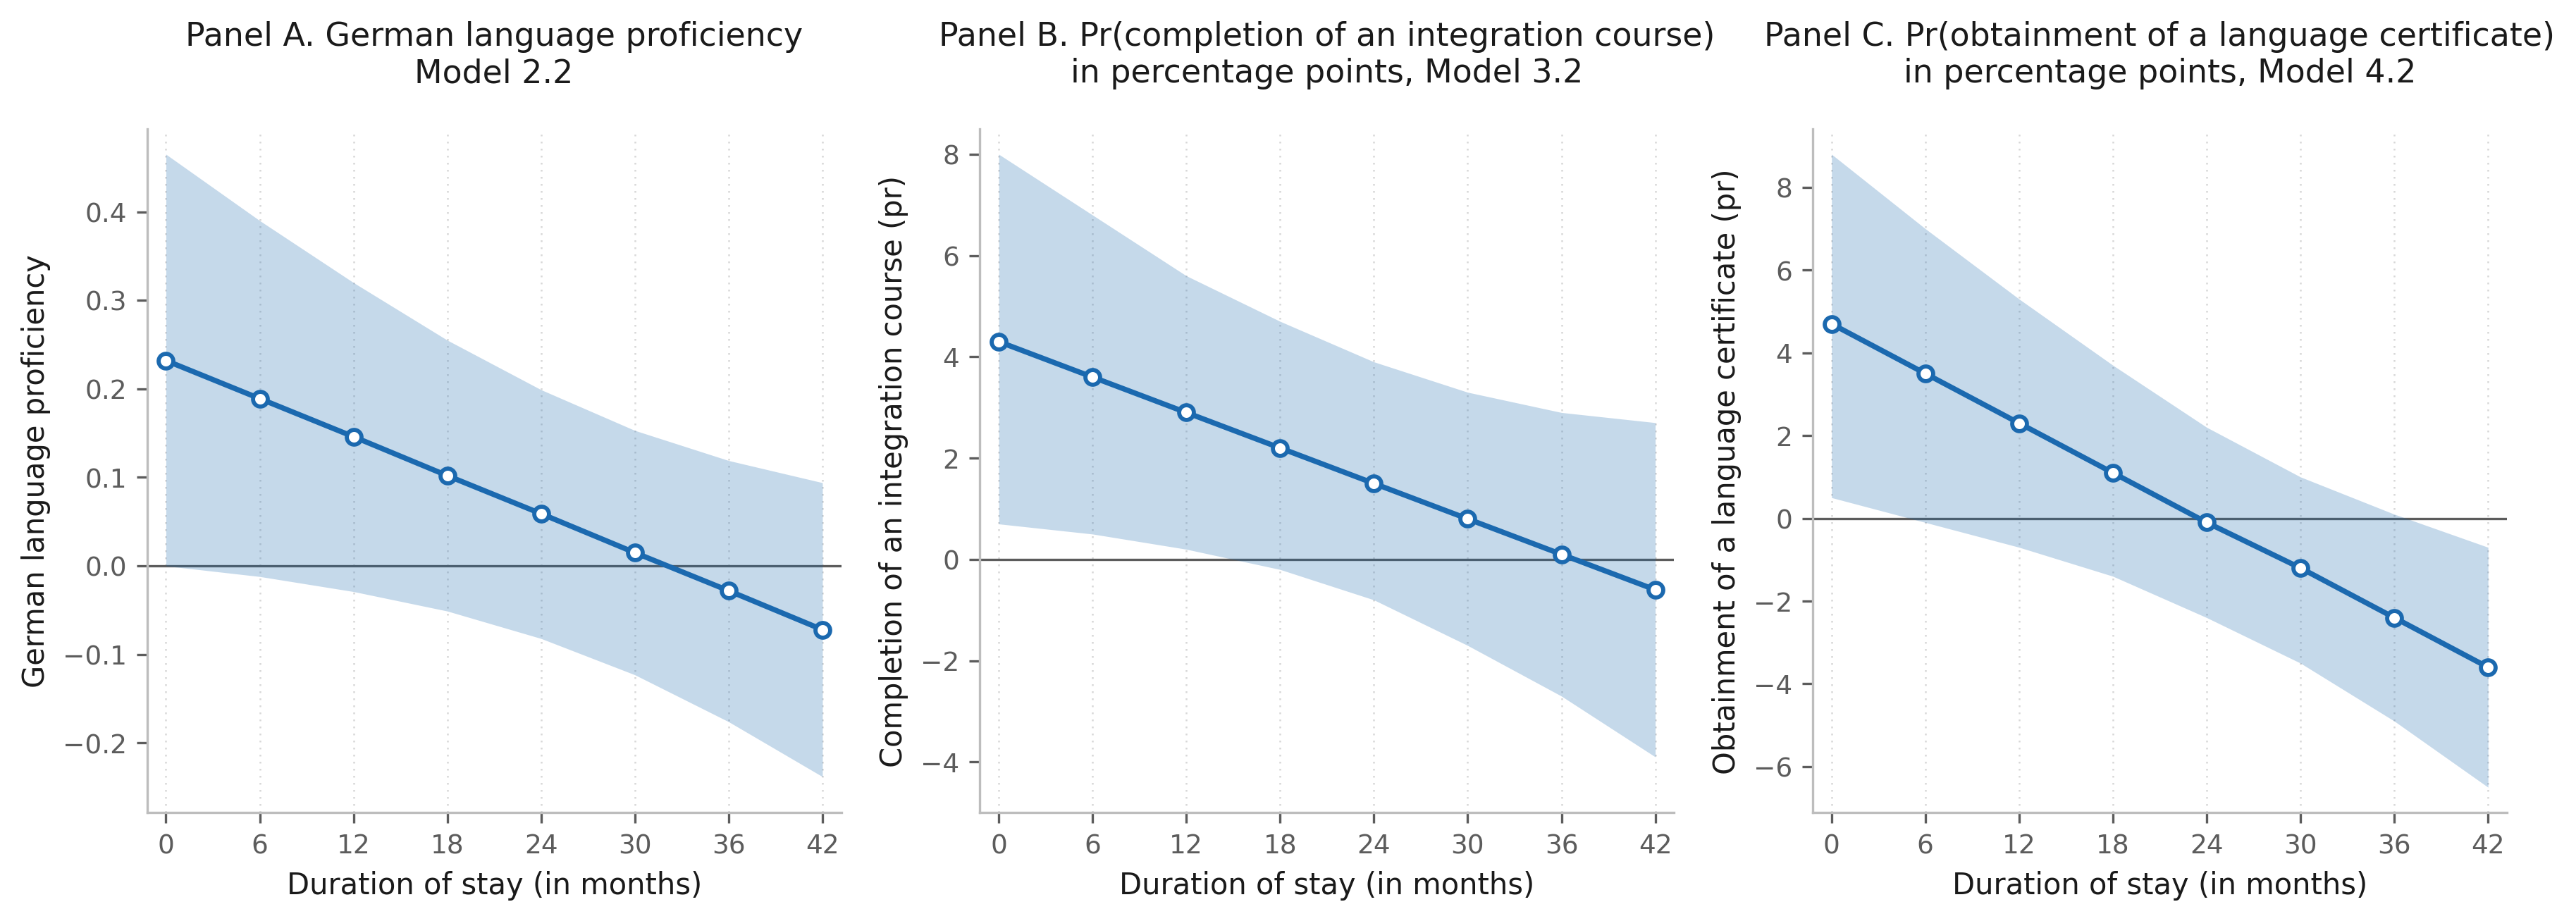
\includegraphics[width=\textwidth]{figures/fig02_all_panels.png}
  \caption[Marginaler Effekt des Kursangebots nach Aufenthaltsdauer]{%
    Durchschnittlicher marginaler Effekt (AME) des Kreisangebots an
    Integrationskursen auf die intermedi\"aren Ergebnisse, nach Aufenthaltsdauer,
    mit 95-\%-Konfidenzintervall. Panel~A: Deutschkenntnisse in Skalenpunkten
    (Modell~2.2); Panel~B: Abschluss eines Integrationskurses in Prozentpunkten
    (Modell~3.2); Panel~C: Erwerb eines Sprachzertifikats in Prozentpunkten
    (Modell~4.2). Zugrunde liegen die Interaktionsmodelle aus
    Tabelle~\ref{tab:intermediaere-ergebnisse}. Eigene Berechnung,
    IAB-BAMF-SOEP-Befragung von Gefl\"uchteten 2016--2019, SOEP-Core v36
    (Remote Edition), gewichtet; N\,=\,5.467 Beobachtungen von 2.730 Personen,
    20~Imputationen. Entspricht Abbildung~2 in \textcite{Kanas:2023}.}
  \label{fig:ame-aufenthaltsdauer}
\end{figure}


\section{Erwerbst\"atigkeit unter Kontrolle der intermedi\"aren Ergebnisse}
\label{sec:erg-mediation}

\textcite{Kanas:2023} haben den Zusammenhang zwischen dem Angebot an Sprachkursen vor Ort und den Beschäftigungschancen von Geflüchteten untersucht und geprüft, ob dieser Zusammenhang auch dann noch besteht, wenn Faktoren wie Kursabschluss, Zertifikat, Deutschkenntnisse und die Häufigkeit des Kontakts zu Deutschen berücksichtigt werden. In Tabelle 5.4 wurde diese Analyse reproduziert, sodass dieselben Ergebnisse ermittelt werden konnten.

Zunächst wird im Modell 1.3 die Deutschkenntnis berücksichtigt. Das Angebot an Kursen erhöht die Beschäftigungswahrscheinlichkeit um fast 3 Prozentpunkte, wenn die Deutschkenntnis dabei berücksichtigt wird. Die Variable „Abschluss des Integrationskurses“ steht in einem positiven Zusammenhang mit der Beschäftigung. Wenn die Variable „Kursabschluss“ in das Modell aufgenommen wird, ist der Effekt des Kursangebots auf die Beschäftigung ebenfalls positiv und statistisch signifikant. Der Besitz eines Deutsch-Sprachzertifikats ist ebenfalls mit einer höheren Beschäftigungswahrscheinlichkeit verbunden, allerdings liegt das statistische Signifikanzniveau bei 10 Prozent. Das bedeutet, dass die Wirkungsstärke dieser Variablen geringer ist als die der Variablen „Abschluss des Integrationskurses“. Auch die Variable „Häufigkeit des Kontakts mit Deutschen“ steht in Zusammenhang mit der Beschäftigungswahrscheinlichkeit, und dieser Zusammenhang ist positiv und signifikant.

In Modell 1.7 und Modell 1.8 wurden mehrere intermediäre Ergebnisse gleichzeitig berücksichtigt. In beiden Modellen lässt sich ein signifikanter und positiver Zusammenhang zwischen der Häufigkeit des Kontakts zu Deutschen und der Beschäftigungswahrscheinlichkeit beobachten. Auch unter Berücksichtigung weiterer intermediärer Variablen blieb der Zusammenhang zwischen der Variable „Kontakt zu Deutschen“ und der Beschäftigungswahrscheinlichkeit stabil. In Modell 1.7 wurde gezeigt, dass der Zusammenhang zwischen dem Abschluss eines Integrationskurses und der Beschäftigungswahrscheinlichkeit auch unter Berücksichtigung der Deutschkenntnisse und der Häufigkeit des Kontakts zu Deutschen signifikant und positiv ist.


% GENERATED BY src/python/lmi/tables/tab05_mediation.py -- DO NOT EDIT
%==============================================================================%
% tab05_mediation.tex
%
% Purpose : Tabelle 5 der Replikation -- Erwerbstaetigkeit unter Kontrolle der
%           intermediaeren Ergebnisse. Entspricht Table 5 in
%           Kanas & Kosyakova, S. 25 (Bib-Key: Kanas:2023).
%           Zweite Tabelle: Gegenueberstellung Publikation vs. Replikation
%           fuer den Anhang.
% Source  : SOEPremote job 244598, src/stata/remote/tab05_mediation.do
%           Rohlisting: results/transcripts/
%                       src_stata_remote_tab05_mediation.do.eml
%           Transkript: results/comparisons/tab05_mediation.md
% Needs   : booktabs, tabularx (beide bereits in bachelorarbeit.sty geladen)
% Usage   : % GENERATED BY src/python/lmi/tables/tab05_mediation.py -- DO NOT EDIT
%==============================================================================%
% tab05_mediation.tex
%
% Purpose : Tabelle 5 der Replikation -- Erwerbstaetigkeit unter Kontrolle der
%           intermediaeren Ergebnisse. Entspricht Table 5 in
%           Kanas & Kosyakova, S. 25 (Bib-Key: Kanas:2023).
%           Zweite Tabelle: Gegenueberstellung Publikation vs. Replikation
%           fuer den Anhang.
% Source  : SOEPremote job 244598, src/stata/remote/tab05_mediation.do
%           Rohlisting: results/transcripts/
%                       src_stata_remote_tab05_mediation.do.eml
%           Transkript: results/comparisons/tab05_mediation.md
% Needs   : booktabs, tabularx (beide bereits in bachelorarbeit.sty geladen)
% Usage   : % GENERATED BY src/python/lmi/tables/tab05_mediation.py -- DO NOT EDIT
%==============================================================================%
% tab05_mediation.tex
%
% Purpose : Tabelle 5 der Replikation -- Erwerbstaetigkeit unter Kontrolle der
%           intermediaeren Ergebnisse. Entspricht Table 5 in
%           Kanas & Kosyakova, S. 25 (Bib-Key: Kanas:2023).
%           Zweite Tabelle: Gegenueberstellung Publikation vs. Replikation
%           fuer den Anhang.
% Source  : SOEPremote job 244598, src/stata/remote/tab05_mediation.do
%           Rohlisting: results/transcripts/
%                       src_stata_remote_tab05_mediation.do.eml
%           Transkript: results/comparisons/tab05_mediation.md
% Needs   : booktabs, tabularx (beide bereits in bachelorarbeit.sty geladen)
% Usage   : \input{tables/tab05_mediation}
% Author  : Emre Suemer, 2026-08-14
%==============================================================================%

\makeatletter
\@ifundefined{NC@rewrite@Z}{%
  \newcolumntype{Z}{>{\raggedright\arraybackslash\hangindent=1.9em\hangafter=1}X}%
}{}
\makeatother

\begin{table}[htbp]
  \centering
  \caption{Erwerbst\"atigkeit und intermedi\"are Ergebnisse}
  \label{tab:mediation}
  \scriptsize
  \setlength{\tabcolsep}{3pt}%
  \begin{tabularx}{\textwidth}{@{}Zrrrrrr@{}}
    \toprule
     & Modell 1.3 & Modell 1.4 & Modell 1.5 & Modell 1.6 & Modell 1.7
     & Modell 1.8 \\
    \midrule
    \textbf{Kreisangebot an Integrationskursen, std.} & 2{,}97$^{*}$ & 2{,}93$^{*}$ & 3{,}04$^{*}$ & 3{,}19$^{**}$ & 3{,}13$^{**}$ & 3{,}18$^{**}$ \\
     & (1{,}18) & (1{,}19) & (1{,}19) & (1{,}12) & (1{,}11) & (1{,}12) \\[0.3ex]
    Aufenthaltsdauer, in Monaten (/12) & 9{,}14$^{**}$ & 10{,}29$^{**}$ & 10{,}32$^{**}$ & 9{,}38$^{**}$ & 8{,}53$^{**}$ & 8{,}68$^{**}$ \\
     & (1{,}62) & (1{,}62) & (1{,}65) & (1{,}61) & (1{,}66) & (1{,}67) \\[0.3ex]
    Deutschkenntnisse & 1{,}64$^{**}$ &  &  &  & 0{,}51 & 0{,}68$^{+}$ \\
     & (0{,}36) &  &  &  & (0{,}37) & (0{,}38) \\[0.3ex]
    Integrationskurs abgeschlossen &  & 7{,}62$^{**}$ &  &  & 6{,}73$^{**}$ &  \\
     &  & (2{,}43) &  &  & (2{,}40) &  \\[0.3ex]
    Sprachzertifikat erworben &  &  & 4{,}02$^{+}$ &  &  & 0{,}81 \\
     &  &  & (2{,}20) &  &  & (2{,}15) \\[0.3ex]
    Kontakth\"aufigkeit zu Deutschen &  &  &  & 5{,}06$^{**}$ & 4{,}88$^{**}$ & 4{,}83$^{**}$ \\
     &  &  &  & (0{,}44) & (0{,}45) & (0{,}45) \\[0.3ex]
    Konstante & $-$10{,}45$^{+}$ & $-$3{,}09 & $-$2{,}70 & $-$18{,}86$^{**}$ & $-$21{,}08$^{**}$ & $-$21{,}39$^{**}$ \\
     & (6{,}26) & (6{,}21) & (6{,}28) & (6{,}16) & (6{,}09) & (6{,}14) \\[0.3ex]
    R\textsuperscript{2} (adj.) & 0{,}2209 & 0{,}2186 & 0{,}2147 & 0{,}2563 & 0{,}2614 & 0{,}2575 \\
    \bottomrule
  \end{tabularx}

  \vspace{0.75ex}
  \parbox{\textwidth}{\footnotesize
    \textit{Anmerkungen:} Eigene Berechnung, IAB-BAMF-SOEP-Befragung von
    Gefl\"uchteten 2016--2019, SOEP-Core v36 (Remote Edition), gewichtet.
    In allen Modellen N\,=\,5.467 Beobachtungen, 2.730 Personen,
    20 Imputationen. Durchschnittliche marginale Effekte in
    Prozentpunkten; robuste, auf Personenebene geclusterte Standardfehler in
    Klammern. Die Kontrollvariablen entsprechen exakt denen aus Modell~1.1 in
    Tabelle~\ref{tab:erwerbstaetigkeit} und sind wie in der Vorlage nicht
    ausgewiesen; die vollst\"andigen Koeffizienten stehen in
    \texttt{build/tables/tab05\_mediation.csv}.
    $^{+}$~p\,$<$\,0{,}1, $^{*}$~p\,$<$\,0{,}05, $^{**}$~p\,$<$\,0{,}01
    (zweiseitig).}
\end{table}


\iffalse
\begin{table}[htbp]
  \centering
  \caption{Tabelle~\ref{tab:mediation} im Vergleich zur Publikation}
  \label{tab:mediation-vergleich}
  \scriptsize
  \setlength{\tabcolsep}{3pt}%
  \begin{tabularx}{\textwidth}{@{}Zrrrrrr@{}}
    \toprule
     & Modell 1.3 & Modell 1.4 & Modell 1.5 & Modell 1.6 & Modell 1.7
     & Modell 1.8 \\
    \midrule
    \multicolumn{7}{@{}l}{\textbf{Publikation}} \\[0.3ex]
    \textbf{Kreisangebot an Integrationskursen, std.} & 2{,}96$^{*}$ & 2{,}91$^{*}$ & 3{,}03$^{*}$ & 3{,}18$^{**}$ & 3{,}12$^{**}$ & 3{,}18$^{**}$ \\
     & (1{,}18) & (1{,}19) & (1{,}20) & (1{,}12) & (1{,}11) & (1{,}12) \\[0.3ex]
    Aufenthaltsdauer, in Monaten (/12) & 9{,}13$^{**}$ & 10{,}27$^{**}$ & 10{,}31$^{**}$ & 9{,}37$^{**}$ & 8{,}51$^{**}$ & 8{,}67$^{**}$ \\
     & (1{,}62) & (1{,}62) & (1{,}64) & (1{,}61) & (1{,}66) & (1{,}67) \\[0.3ex]
    Deutschkenntnisse & 1{,}65$^{**}$ &  &  &  & 0{,}51 & 0{,}69$^{+}$ \\
     & (0{,}37) &  &  &  & (0{,}37) & (0{,}38) \\[0.3ex]
    Integrationskurs abgeschlossen &  & 7{,}95$^{**}$ &  &  & 7{,}02$^{**}$ &  \\
     &  & (2{,}41) &  &  & (2{,}38) &  \\[0.3ex]
    Sprachzertifikat erworben &  &  & 4{,}09$^{+}$ &  &  & 0{,}86 \\
     &  &  & (2{,}20) &  &  & (2{,}15) \\[0.3ex]
    Kontakth\"aufigkeit zu Deutschen &  &  &  & 5{,}07$^{**}$ & 4{,}87$^{**}$ & 4{,}83$^{**}$ \\
     &  &  &  & (0{,}44) & (0{,}45) & (0{,}46) \\[0.3ex]
    Konstante & $-$10{,}35$^{+}$ & $-$2{,}87 & $-$2{,}49 & $-$18{,}58$^{**}$ & $-$20{,}83$^{**}$ & $-$21{,}17$^{**}$ \\
     & (6{,}25) & (6{,}19) & (6{,}26) & (6{,}18) & (6{,}12) & (6{,}17) \\[0.3ex]
    R\textsuperscript{2} (adj.) & 0{,}2205 & 0{,}2185 & 0{,}2143 & 0{,}2558 & 0{,}2613 & 0{,}2571 \\
    \midrule
    \multicolumn{7}{@{}l}{\textbf{Replikation}} \\[0.3ex]
    \textbf{Kreisangebot an Integrationskursen, std.} & 2{,}97$^{*}$ & 2{,}93$^{*}$ & 3{,}04$^{*}$ & 3{,}19$^{**}$ & 3{,}13$^{**}$ & 3{,}18$^{**}$ \\
     & (1{,}18) & (1{,}19) & (1{,}19) & (1{,}12) & (1{,}11) & (1{,}12) \\[0.3ex]
    Aufenthaltsdauer, in Monaten (/12) & 9{,}14$^{**}$ & 10{,}29$^{**}$ & 10{,}32$^{**}$ & 9{,}38$^{**}$ & 8{,}53$^{**}$ & 8{,}68$^{**}$ \\
     & (1{,}62) & (1{,}62) & (1{,}65) & (1{,}61) & (1{,}66) & (1{,}67) \\[0.3ex]
    Deutschkenntnisse & 1{,}64$^{**}$ &  &  &  & 0{,}51 & 0{,}68$^{+}$ \\
     & (0{,}36) &  &  &  & (0{,}37) & (0{,}38) \\[0.3ex]
    Integrationskurs abgeschlossen &  & 7{,}62$^{**}$ &  &  & 6{,}73$^{**}$ &  \\
     &  & (2{,}43) &  &  & (2{,}40) &  \\[0.3ex]
    Sprachzertifikat erworben &  &  & 4{,}02$^{+}$ &  &  & 0{,}81 \\
     &  &  & (2{,}20) &  &  & (2{,}15) \\[0.3ex]
    Kontakth\"aufigkeit zu Deutschen &  &  &  & 5{,}06$^{**}$ & 4{,}88$^{**}$ & 4{,}83$^{**}$ \\
     &  &  &  & (0{,}44) & (0{,}45) & (0{,}45) \\[0.3ex]
    Konstante & $-$10{,}45$^{+}$ & $-$3{,}09 & $-$2{,}70 & $-$18{,}86$^{**}$ & $-$21{,}08$^{**}$ & $-$21{,}39$^{**}$ \\
     & (6{,}26) & (6{,}21) & (6{,}28) & (6{,}16) & (6{,}09) & (6{,}14) \\[0.3ex]
    R\textsuperscript{2} (adj.) & 0{,}2209 & 0{,}2186 & 0{,}2147 & 0{,}2563 & 0{,}2614 & 0{,}2575 \\
    \bottomrule
  \end{tabularx}

  \vspace{0.75ex}
  \parbox{\textwidth}{\footnotesize
    \textit{Anmerkungen:} Publizierte Werte aus \textcite[25]{Kanas:2023},
    eigene Werte aus SOEPremote-Job~244598. Einheiten wie oben.
    Gr\"o\ss{}te Abweichung des Treatment-Koeffizienten: 0{,}02\,p.p.;
    gr\"o\ss{}te Abweichung eines Steigungskoeffizienten: 0{,}33\,p.p.;
    gr\"o\ss{}te Abweichung insgesamt: 0{,}33\,p.p.
    Alle Signifikanzniveaus stimmen \"uberein.
    \\[0.4ex]
    \textbf{Anmerkung:} Die Fiskalrechnung der Autorinnen st\"utzt sich auf
    Modell~1.7, nicht auf den Haupteffekt aus
    Tabelle~\ref{tab:erwerbstaetigkeit}: 3{,}13\,p.p. $\times$ 10.000 $\times$ 4.800\,Euro = 1.502.400\,Euro (publiziert: 1.497.600\,Euro).}
\end{table}
\fi
% Author  : Emre Suemer, 2026-08-14
%==============================================================================%

\makeatletter
\@ifundefined{NC@rewrite@Z}{%
  \newcolumntype{Z}{>{\raggedright\arraybackslash\hangindent=1.9em\hangafter=1}X}%
}{}
\makeatother

\begin{table}[htbp]
  \centering
  \caption{Erwerbst\"atigkeit und intermedi\"are Ergebnisse}
  \label{tab:mediation}
  \scriptsize
  \setlength{\tabcolsep}{3pt}%
  \begin{tabularx}{\textwidth}{@{}Zrrrrrr@{}}
    \toprule
     & Modell 1.3 & Modell 1.4 & Modell 1.5 & Modell 1.6 & Modell 1.7
     & Modell 1.8 \\
    \midrule
    \textbf{Kreisangebot an Integrationskursen, std.} & 2{,}97$^{*}$ & 2{,}93$^{*}$ & 3{,}04$^{*}$ & 3{,}19$^{**}$ & 3{,}13$^{**}$ & 3{,}18$^{**}$ \\
     & (1{,}18) & (1{,}19) & (1{,}19) & (1{,}12) & (1{,}11) & (1{,}12) \\[0.3ex]
    Aufenthaltsdauer, in Monaten (/12) & 9{,}14$^{**}$ & 10{,}29$^{**}$ & 10{,}32$^{**}$ & 9{,}38$^{**}$ & 8{,}53$^{**}$ & 8{,}68$^{**}$ \\
     & (1{,}62) & (1{,}62) & (1{,}65) & (1{,}61) & (1{,}66) & (1{,}67) \\[0.3ex]
    Deutschkenntnisse & 1{,}64$^{**}$ &  &  &  & 0{,}51 & 0{,}68$^{+}$ \\
     & (0{,}36) &  &  &  & (0{,}37) & (0{,}38) \\[0.3ex]
    Integrationskurs abgeschlossen &  & 7{,}62$^{**}$ &  &  & 6{,}73$^{**}$ &  \\
     &  & (2{,}43) &  &  & (2{,}40) &  \\[0.3ex]
    Sprachzertifikat erworben &  &  & 4{,}02$^{+}$ &  &  & 0{,}81 \\
     &  &  & (2{,}20) &  &  & (2{,}15) \\[0.3ex]
    Kontakth\"aufigkeit zu Deutschen &  &  &  & 5{,}06$^{**}$ & 4{,}88$^{**}$ & 4{,}83$^{**}$ \\
     &  &  &  & (0{,}44) & (0{,}45) & (0{,}45) \\[0.3ex]
    Konstante & $-$10{,}45$^{+}$ & $-$3{,}09 & $-$2{,}70 & $-$18{,}86$^{**}$ & $-$21{,}08$^{**}$ & $-$21{,}39$^{**}$ \\
     & (6{,}26) & (6{,}21) & (6{,}28) & (6{,}16) & (6{,}09) & (6{,}14) \\[0.3ex]
    R\textsuperscript{2} (adj.) & 0{,}2209 & 0{,}2186 & 0{,}2147 & 0{,}2563 & 0{,}2614 & 0{,}2575 \\
    \bottomrule
  \end{tabularx}

  \vspace{0.75ex}
  \parbox{\textwidth}{\footnotesize
    \textit{Anmerkungen:} Eigene Berechnung, IAB-BAMF-SOEP-Befragung von
    Gefl\"uchteten 2016--2019, SOEP-Core v36 (Remote Edition), gewichtet.
    In allen Modellen N\,=\,5.467 Beobachtungen, 2.730 Personen,
    20 Imputationen. Durchschnittliche marginale Effekte in
    Prozentpunkten; robuste, auf Personenebene geclusterte Standardfehler in
    Klammern. Die Kontrollvariablen entsprechen exakt denen aus Modell~1.1 in
    Tabelle~\ref{tab:erwerbstaetigkeit} und sind wie in der Vorlage nicht
    ausgewiesen; die vollst\"andigen Koeffizienten stehen in
    \texttt{build/tables/tab05\_mediation.csv}.
    $^{+}$~p\,$<$\,0{,}1, $^{*}$~p\,$<$\,0{,}05, $^{**}$~p\,$<$\,0{,}01
    (zweiseitig).}
\end{table}


\iffalse
\begin{table}[htbp]
  \centering
  \caption{Tabelle~\ref{tab:mediation} im Vergleich zur Publikation}
  \label{tab:mediation-vergleich}
  \scriptsize
  \setlength{\tabcolsep}{3pt}%
  \begin{tabularx}{\textwidth}{@{}Zrrrrrr@{}}
    \toprule
     & Modell 1.3 & Modell 1.4 & Modell 1.5 & Modell 1.6 & Modell 1.7
     & Modell 1.8 \\
    \midrule
    \multicolumn{7}{@{}l}{\textbf{Publikation}} \\[0.3ex]
    \textbf{Kreisangebot an Integrationskursen, std.} & 2{,}96$^{*}$ & 2{,}91$^{*}$ & 3{,}03$^{*}$ & 3{,}18$^{**}$ & 3{,}12$^{**}$ & 3{,}18$^{**}$ \\
     & (1{,}18) & (1{,}19) & (1{,}20) & (1{,}12) & (1{,}11) & (1{,}12) \\[0.3ex]
    Aufenthaltsdauer, in Monaten (/12) & 9{,}13$^{**}$ & 10{,}27$^{**}$ & 10{,}31$^{**}$ & 9{,}37$^{**}$ & 8{,}51$^{**}$ & 8{,}67$^{**}$ \\
     & (1{,}62) & (1{,}62) & (1{,}64) & (1{,}61) & (1{,}66) & (1{,}67) \\[0.3ex]
    Deutschkenntnisse & 1{,}65$^{**}$ &  &  &  & 0{,}51 & 0{,}69$^{+}$ \\
     & (0{,}37) &  &  &  & (0{,}37) & (0{,}38) \\[0.3ex]
    Integrationskurs abgeschlossen &  & 7{,}95$^{**}$ &  &  & 7{,}02$^{**}$ &  \\
     &  & (2{,}41) &  &  & (2{,}38) &  \\[0.3ex]
    Sprachzertifikat erworben &  &  & 4{,}09$^{+}$ &  &  & 0{,}86 \\
     &  &  & (2{,}20) &  &  & (2{,}15) \\[0.3ex]
    Kontakth\"aufigkeit zu Deutschen &  &  &  & 5{,}07$^{**}$ & 4{,}87$^{**}$ & 4{,}83$^{**}$ \\
     &  &  &  & (0{,}44) & (0{,}45) & (0{,}46) \\[0.3ex]
    Konstante & $-$10{,}35$^{+}$ & $-$2{,}87 & $-$2{,}49 & $-$18{,}58$^{**}$ & $-$20{,}83$^{**}$ & $-$21{,}17$^{**}$ \\
     & (6{,}25) & (6{,}19) & (6{,}26) & (6{,}18) & (6{,}12) & (6{,}17) \\[0.3ex]
    R\textsuperscript{2} (adj.) & 0{,}2205 & 0{,}2185 & 0{,}2143 & 0{,}2558 & 0{,}2613 & 0{,}2571 \\
    \midrule
    \multicolumn{7}{@{}l}{\textbf{Replikation}} \\[0.3ex]
    \textbf{Kreisangebot an Integrationskursen, std.} & 2{,}97$^{*}$ & 2{,}93$^{*}$ & 3{,}04$^{*}$ & 3{,}19$^{**}$ & 3{,}13$^{**}$ & 3{,}18$^{**}$ \\
     & (1{,}18) & (1{,}19) & (1{,}19) & (1{,}12) & (1{,}11) & (1{,}12) \\[0.3ex]
    Aufenthaltsdauer, in Monaten (/12) & 9{,}14$^{**}$ & 10{,}29$^{**}$ & 10{,}32$^{**}$ & 9{,}38$^{**}$ & 8{,}53$^{**}$ & 8{,}68$^{**}$ \\
     & (1{,}62) & (1{,}62) & (1{,}65) & (1{,}61) & (1{,}66) & (1{,}67) \\[0.3ex]
    Deutschkenntnisse & 1{,}64$^{**}$ &  &  &  & 0{,}51 & 0{,}68$^{+}$ \\
     & (0{,}36) &  &  &  & (0{,}37) & (0{,}38) \\[0.3ex]
    Integrationskurs abgeschlossen &  & 7{,}62$^{**}$ &  &  & 6{,}73$^{**}$ &  \\
     &  & (2{,}43) &  &  & (2{,}40) &  \\[0.3ex]
    Sprachzertifikat erworben &  &  & 4{,}02$^{+}$ &  &  & 0{,}81 \\
     &  &  & (2{,}20) &  &  & (2{,}15) \\[0.3ex]
    Kontakth\"aufigkeit zu Deutschen &  &  &  & 5{,}06$^{**}$ & 4{,}88$^{**}$ & 4{,}83$^{**}$ \\
     &  &  &  & (0{,}44) & (0{,}45) & (0{,}45) \\[0.3ex]
    Konstante & $-$10{,}45$^{+}$ & $-$3{,}09 & $-$2{,}70 & $-$18{,}86$^{**}$ & $-$21{,}08$^{**}$ & $-$21{,}39$^{**}$ \\
     & (6{,}26) & (6{,}21) & (6{,}28) & (6{,}16) & (6{,}09) & (6{,}14) \\[0.3ex]
    R\textsuperscript{2} (adj.) & 0{,}2209 & 0{,}2186 & 0{,}2147 & 0{,}2563 & 0{,}2614 & 0{,}2575 \\
    \bottomrule
  \end{tabularx}

  \vspace{0.75ex}
  \parbox{\textwidth}{\footnotesize
    \textit{Anmerkungen:} Publizierte Werte aus \textcite[25]{Kanas:2023},
    eigene Werte aus SOEPremote-Job~244598. Einheiten wie oben.
    Gr\"o\ss{}te Abweichung des Treatment-Koeffizienten: 0{,}02\,p.p.;
    gr\"o\ss{}te Abweichung eines Steigungskoeffizienten: 0{,}33\,p.p.;
    gr\"o\ss{}te Abweichung insgesamt: 0{,}33\,p.p.
    Alle Signifikanzniveaus stimmen \"uberein.
    \\[0.4ex]
    \textbf{Anmerkung:} Die Fiskalrechnung der Autorinnen st\"utzt sich auf
    Modell~1.7, nicht auf den Haupteffekt aus
    Tabelle~\ref{tab:erwerbstaetigkeit}: 3{,}13\,p.p. $\times$ 10.000 $\times$ 4.800\,Euro = 1.502.400\,Euro (publiziert: 1.497.600\,Euro).}
\end{table}
\fi
% Author  : Emre Suemer, 2026-08-14
%==============================================================================%

\makeatletter
\@ifundefined{NC@rewrite@Z}{%
  \newcolumntype{Z}{>{\raggedright\arraybackslash\hangindent=1.9em\hangafter=1}X}%
}{}
\makeatother

\begin{table}[htbp]
  \centering
  \caption{Erwerbst\"atigkeit und intermedi\"are Ergebnisse}
  \label{tab:mediation}
  \scriptsize
  \setlength{\tabcolsep}{3pt}%
  \begin{tabularx}{\textwidth}{@{}Zrrrrrr@{}}
    \toprule
     & Modell 1.3 & Modell 1.4 & Modell 1.5 & Modell 1.6 & Modell 1.7
     & Modell 1.8 \\
    \midrule
    \textbf{Kreisangebot an Integrationskursen, std.} & 2{,}97$^{*}$ & 2{,}93$^{*}$ & 3{,}04$^{*}$ & 3{,}19$^{**}$ & 3{,}13$^{**}$ & 3{,}18$^{**}$ \\
     & (1{,}18) & (1{,}19) & (1{,}19) & (1{,}12) & (1{,}11) & (1{,}12) \\[0.3ex]
    Aufenthaltsdauer, in Monaten (/12) & 9{,}14$^{**}$ & 10{,}29$^{**}$ & 10{,}32$^{**}$ & 9{,}38$^{**}$ & 8{,}53$^{**}$ & 8{,}68$^{**}$ \\
     & (1{,}62) & (1{,}62) & (1{,}65) & (1{,}61) & (1{,}66) & (1{,}67) \\[0.3ex]
    Deutschkenntnisse & 1{,}64$^{**}$ &  &  &  & 0{,}51 & 0{,}68$^{+}$ \\
     & (0{,}36) &  &  &  & (0{,}37) & (0{,}38) \\[0.3ex]
    Integrationskurs abgeschlossen &  & 7{,}62$^{**}$ &  &  & 6{,}73$^{**}$ &  \\
     &  & (2{,}43) &  &  & (2{,}40) &  \\[0.3ex]
    Sprachzertifikat erworben &  &  & 4{,}02$^{+}$ &  &  & 0{,}81 \\
     &  &  & (2{,}20) &  &  & (2{,}15) \\[0.3ex]
    Kontakth\"aufigkeit zu Deutschen &  &  &  & 5{,}06$^{**}$ & 4{,}88$^{**}$ & 4{,}83$^{**}$ \\
     &  &  &  & (0{,}44) & (0{,}45) & (0{,}45) \\[0.3ex]
    Konstante & $-$10{,}45$^{+}$ & $-$3{,}09 & $-$2{,}70 & $-$18{,}86$^{**}$ & $-$21{,}08$^{**}$ & $-$21{,}39$^{**}$ \\
     & (6{,}26) & (6{,}21) & (6{,}28) & (6{,}16) & (6{,}09) & (6{,}14) \\[0.3ex]
    R\textsuperscript{2} (adj.) & 0{,}2209 & 0{,}2186 & 0{,}2147 & 0{,}2563 & 0{,}2614 & 0{,}2575 \\
    \bottomrule
  \end{tabularx}

  \vspace{0.75ex}
  \parbox{\textwidth}{\footnotesize
    \textit{Anmerkungen:} Eigene Berechnung, IAB-BAMF-SOEP-Befragung von
    Gefl\"uchteten 2016--2019, SOEP-Core v36 (Remote Edition), gewichtet.
    In allen Modellen N\,=\,5.467 Beobachtungen, 2.730 Personen,
    20 Imputationen. Durchschnittliche marginale Effekte in
    Prozentpunkten; robuste, auf Personenebene geclusterte Standardfehler in
    Klammern. Die Kontrollvariablen entsprechen exakt denen aus Modell~1.1 in
    Tabelle~\ref{tab:erwerbstaetigkeit} und sind wie in der Vorlage nicht
    ausgewiesen; die vollst\"andigen Koeffizienten stehen in
    \texttt{build/tables/tab05\_mediation.csv}.
    $^{+}$~p\,$<$\,0{,}1, $^{*}$~p\,$<$\,0{,}05, $^{**}$~p\,$<$\,0{,}01
    (zweiseitig).}
\end{table}


\iffalse
\begin{table}[htbp]
  \centering
  \caption{Tabelle~\ref{tab:mediation} im Vergleich zur Publikation}
  \label{tab:mediation-vergleich}
  \scriptsize
  \setlength{\tabcolsep}{3pt}%
  \begin{tabularx}{\textwidth}{@{}Zrrrrrr@{}}
    \toprule
     & Modell 1.3 & Modell 1.4 & Modell 1.5 & Modell 1.6 & Modell 1.7
     & Modell 1.8 \\
    \midrule
    \multicolumn{7}{@{}l}{\textbf{Publikation}} \\[0.3ex]
    \textbf{Kreisangebot an Integrationskursen, std.} & 2{,}96$^{*}$ & 2{,}91$^{*}$ & 3{,}03$^{*}$ & 3{,}18$^{**}$ & 3{,}12$^{**}$ & 3{,}18$^{**}$ \\
     & (1{,}18) & (1{,}19) & (1{,}20) & (1{,}12) & (1{,}11) & (1{,}12) \\[0.3ex]
    Aufenthaltsdauer, in Monaten (/12) & 9{,}13$^{**}$ & 10{,}27$^{**}$ & 10{,}31$^{**}$ & 9{,}37$^{**}$ & 8{,}51$^{**}$ & 8{,}67$^{**}$ \\
     & (1{,}62) & (1{,}62) & (1{,}64) & (1{,}61) & (1{,}66) & (1{,}67) \\[0.3ex]
    Deutschkenntnisse & 1{,}65$^{**}$ &  &  &  & 0{,}51 & 0{,}69$^{+}$ \\
     & (0{,}37) &  &  &  & (0{,}37) & (0{,}38) \\[0.3ex]
    Integrationskurs abgeschlossen &  & 7{,}95$^{**}$ &  &  & 7{,}02$^{**}$ &  \\
     &  & (2{,}41) &  &  & (2{,}38) &  \\[0.3ex]
    Sprachzertifikat erworben &  &  & 4{,}09$^{+}$ &  &  & 0{,}86 \\
     &  &  & (2{,}20) &  &  & (2{,}15) \\[0.3ex]
    Kontakth\"aufigkeit zu Deutschen &  &  &  & 5{,}07$^{**}$ & 4{,}87$^{**}$ & 4{,}83$^{**}$ \\
     &  &  &  & (0{,}44) & (0{,}45) & (0{,}46) \\[0.3ex]
    Konstante & $-$10{,}35$^{+}$ & $-$2{,}87 & $-$2{,}49 & $-$18{,}58$^{**}$ & $-$20{,}83$^{**}$ & $-$21{,}17$^{**}$ \\
     & (6{,}25) & (6{,}19) & (6{,}26) & (6{,}18) & (6{,}12) & (6{,}17) \\[0.3ex]
    R\textsuperscript{2} (adj.) & 0{,}2205 & 0{,}2185 & 0{,}2143 & 0{,}2558 & 0{,}2613 & 0{,}2571 \\
    \midrule
    \multicolumn{7}{@{}l}{\textbf{Replikation}} \\[0.3ex]
    \textbf{Kreisangebot an Integrationskursen, std.} & 2{,}97$^{*}$ & 2{,}93$^{*}$ & 3{,}04$^{*}$ & 3{,}19$^{**}$ & 3{,}13$^{**}$ & 3{,}18$^{**}$ \\
     & (1{,}18) & (1{,}19) & (1{,}19) & (1{,}12) & (1{,}11) & (1{,}12) \\[0.3ex]
    Aufenthaltsdauer, in Monaten (/12) & 9{,}14$^{**}$ & 10{,}29$^{**}$ & 10{,}32$^{**}$ & 9{,}38$^{**}$ & 8{,}53$^{**}$ & 8{,}68$^{**}$ \\
     & (1{,}62) & (1{,}62) & (1{,}65) & (1{,}61) & (1{,}66) & (1{,}67) \\[0.3ex]
    Deutschkenntnisse & 1{,}64$^{**}$ &  &  &  & 0{,}51 & 0{,}68$^{+}$ \\
     & (0{,}36) &  &  &  & (0{,}37) & (0{,}38) \\[0.3ex]
    Integrationskurs abgeschlossen &  & 7{,}62$^{**}$ &  &  & 6{,}73$^{**}$ &  \\
     &  & (2{,}43) &  &  & (2{,}40) &  \\[0.3ex]
    Sprachzertifikat erworben &  &  & 4{,}02$^{+}$ &  &  & 0{,}81 \\
     &  &  & (2{,}20) &  &  & (2{,}15) \\[0.3ex]
    Kontakth\"aufigkeit zu Deutschen &  &  &  & 5{,}06$^{**}$ & 4{,}88$^{**}$ & 4{,}83$^{**}$ \\
     &  &  &  & (0{,}44) & (0{,}45) & (0{,}45) \\[0.3ex]
    Konstante & $-$10{,}45$^{+}$ & $-$3{,}09 & $-$2{,}70 & $-$18{,}86$^{**}$ & $-$21{,}08$^{**}$ & $-$21{,}39$^{**}$ \\
     & (6{,}26) & (6{,}21) & (6{,}28) & (6{,}16) & (6{,}09) & (6{,}14) \\[0.3ex]
    R\textsuperscript{2} (adj.) & 0{,}2209 & 0{,}2186 & 0{,}2147 & 0{,}2563 & 0{,}2614 & 0{,}2575 \\
    \bottomrule
  \end{tabularx}

  \vspace{0.75ex}
  \parbox{\textwidth}{\footnotesize
    \textit{Anmerkungen:} Publizierte Werte aus \textcite[25]{Kanas:2023},
    eigene Werte aus SOEPremote-Job~244598. Einheiten wie oben.
    Gr\"o\ss{}te Abweichung des Treatment-Koeffizienten: 0{,}02\,p.p.;
    gr\"o\ss{}te Abweichung eines Steigungskoeffizienten: 0{,}33\,p.p.;
    gr\"o\ss{}te Abweichung insgesamt: 0{,}33\,p.p.
    Alle Signifikanzniveaus stimmen \"uberein.
    \\[0.4ex]
    \textbf{Anmerkung:} Die Fiskalrechnung der Autorinnen st\"utzt sich auf
    Modell~1.7, nicht auf den Haupteffekt aus
    Tabelle~\ref{tab:erwerbstaetigkeit}: 3{,}13\,p.p. $\times$ 10.000 $\times$ 4.800\,Euro = 1.502.400\,Euro (publiziert: 1.497.600\,Euro).}
\end{table}
\fi




%\section{Erweiterte Ergebnisse}
%\label{sec:erw-erg}


\subsection{Ergebnisse der Erweiterung}
\label{sec:erg-erweiterung}

Dieser Abschnitt untersucht, ob sich die Auswirkungen des Kursangebots auf die Beschäftigung je nach Asylstatus der Geflüchteten unterscheiden. \textcite{Kanas:2023} analysierten, ob sich die Auswirkungen des Kursangebots auf die Beschäftigung je nach Asylstatus unterscheiden. Die Erweiterung dieser Studie berücksichtigt die Interaktion zwischen dem lokalen Kursangebot und dem Asylstatus im Hinblick auf die Kursmechanismen. Die Interaktion zwischen dem lokalen Kursangebot und dem Asylstatus wird im Hinblick auf die Auswirkungen auf den Kursabschluss, den Erwerb eines Zertifikats und die Deutschkenntnisse untersucht. Damit wird in dieser Arbeit analysiert, ob Flüchtlinge je nach Asylstatus in unterschiedlichem Maße von lokalen Sprachkursen im Hinblick auf diese Integrationsmechanismen profitieren.

Im ersten Teil dieses Kapitels werden die Ergebnisse dargelegt, ob sich die Auswirkungen des lokalen Kursangebots auf die Beschäftigung je nach Asylstatus unterscheiden. Außerdem wird der marginale Effekt des Kursangebots für jeden einzelnen Asylstatus erläutert. Anhand von Tabelle 5.8 wird die Reproduzierbarkeit der Ergebnisse von \textcite{Kanas:2023} überprüft. In Tabelle 5.9 wurde die Analyse auf die Mechanismen der Integration ausgeweitet und es werden die Ergebnisse zu den marginalen Effekten des Kursangebots je nach Asylstatus dargestellt. Tabelle 5.10 zeigt hingegen die grundlegenden Regressionskoeffizienten sowie die Interaktionseffekte der Mechanismenanalysen. Schließlich zeigt Tabelle 5.11 Ergebnisse dazu, ob die Auswirkungen des Kursangebots auf die Beschäftigung und die Deutschkenntnisse sowohl vom Asylstatus als auch von der Aufenthaltsdauer in Deutschland abhängen.

Tabelle 5.6 zeigt den marginalen Effekt auf die Erwerbstätigkeit in Prozentpunkten. Das Modell E1.1 misst den Asylstatus im Erhebungsjahr. Das Modell E1.2 hingegen misst den Status zum Zeitpunkt der ersten Erhebung. Da im zweiten Modell die zeitliche Abfolge zwischen der Zuweisung zu einem Landkreis und der Asylentscheidung berücksichtigt wird, ist es im Kontext der Forschungsfrage von Bedeutung. Der grundlegende Effekt des Kursangebots erweist sich als positiv und statistisch signifikant. Ein Anstieg des Kursangebots um eine Standardabweichung in dem Kreis, dem eine Person zugeordnet ist, erhöht die Wahrscheinlichkeit einer Beschäftigung um 4,25 Prozentpunkte. Damit wurde das zentrale Ergebnis von Kanas und Kosyakova auch unter erweiterten Bedingungen geprüft.

Im Zusammenhang mit der Forschungsfrage dieser Arbeit spielt die Interaktion zwischen Kursangebot und Asylstatus eine zentrale Rolle. Diese Interaktion ist in beiden Modellen statistisch nicht signifikant (E1.1: −1,28; E1.2: −2,87). Es gibt daher keinen Hinweis darauf, dass die Gruppe „Annerkannt“ im Vergleich zur Referenzgruppe stärker vom Kursangebot beeinflusst wird. Die Annahme, dass anerkannte Geflüchtete stärker vom lokalen Kursangebot profitieren, wird aus diesem Grund nicht gestützt. Außerdem sind die gemeinsamen Interaktionen beider Tests nicht signifikant. Im Modell E1.2 liegt lediglich eine schwache Signifikanz vor (p = 0,084). Der Interaktionseffekt im Modell E1.2 ist bei Personen mit abgelehntem Status negativ und statistisch signifikant (−5,13*). Daraus ergibt sich die Erkenntnis, dass bei Personen mit abgelehntem Asylantrag die Auswirkungen des Kursangebots auf die Beschäftigung im Vergleich zur Referenzgruppe geringer sind.

Insgesamt wurde die Analyse von \textcite{Kanas:2023} mit dem Modell E.1.1 wiederholt und überprüft. Im Modell E1.2 wurde der Asylstatus als erster Beobachtungszustand gemessen. Zusammenfassend lässt sich feststellen, dass der grundlegende Effekt des Kursangebots signifikant ist. Berücksichtigt man jedoch den Asylstatus als erste Beobachtungssituation, ist dieser Effekt statistisch nicht signifikant. Daher lässt sich keine Abhängigkeit des Einflusses des Kursangebots auf die Beschäftigung vom jeweiligen Asylstatus feststellen.

% GENERATED BY src/python/lmi/tables/ext_asyl_employment.py
% -- DO NOT EDIT
%==============================================================================%
% ext_asyl_employment.tex
%
% Purpose : Erweiterung, Tabelle E1 -- Kursangebot x Asylstatus auf die
%           Erwerbstaetigkeit. Drei Tabellen: Koeffizienten, marginale Effekte
%           je Statusgruppe, sowie der Vergleich mit Tabelle S6 Modell 1.1.9
%           der Publikation, die dieser Job mitrepliziert.
% Source  : SOEPremote job 244835, src/stata/remote/ext_asyl_employment.do
%           Rohlisting: results/transcripts/
%                       src_stata_remote_ext_asyl_employment.do.eml
%           Transkript: results/comparisons/ext_asyl_employment.md
% Needs   : booktabs, tabularx (beide bereits in bachelorarbeit.sty geladen)
% Usage   : % GENERATED BY src/python/lmi/tables/ext_asyl_employment.py
% -- DO NOT EDIT
%==============================================================================%
% ext_asyl_employment.tex
%
% Purpose : Erweiterung, Tabelle E1 -- Kursangebot x Asylstatus auf die
%           Erwerbstaetigkeit. Drei Tabellen: Koeffizienten, marginale Effekte
%           je Statusgruppe, sowie der Vergleich mit Tabelle S6 Modell 1.1.9
%           der Publikation, die dieser Job mitrepliziert.
% Source  : SOEPremote job 244835, src/stata/remote/ext_asyl_employment.do
%           Rohlisting: results/transcripts/
%                       src_stata_remote_ext_asyl_employment.do.eml
%           Transkript: results/comparisons/ext_asyl_employment.md
% Needs   : booktabs, tabularx (beide bereits in bachelorarbeit.sty geladen)
% Usage   : % GENERATED BY src/python/lmi/tables/ext_asyl_employment.py
% -- DO NOT EDIT
%==============================================================================%
% ext_asyl_employment.tex
%
% Purpose : Erweiterung, Tabelle E1 -- Kursangebot x Asylstatus auf die
%           Erwerbstaetigkeit. Drei Tabellen: Koeffizienten, marginale Effekte
%           je Statusgruppe, sowie der Vergleich mit Tabelle S6 Modell 1.1.9
%           der Publikation, die dieser Job mitrepliziert.
% Source  : SOEPremote job 244835, src/stata/remote/ext_asyl_employment.do
%           Rohlisting: results/transcripts/
%                       src_stata_remote_ext_asyl_employment.do.eml
%           Transkript: results/comparisons/ext_asyl_employment.md
% Needs   : booktabs, tabularx (beide bereits in bachelorarbeit.sty geladen)
% Usage   : \input{tables/ext_asyl_employment}
% Author  : Emre Suemer, 2026-09-01
%==============================================================================%

\makeatletter
\@ifundefined{NC@rewrite@Z}{%
  \newcolumntype{Z}{>{\raggedright\arraybackslash\hangindent=1.9em\hangafter=1}X}%
}{}
\makeatother

\begin{table}[htbp]
  \centering
  \caption{Kursangebot und Asylstatus: Wahrscheinlichkeit bezahlter Arbeit}
  \label{tab:ext-asyl-erwerb}
  \footnotesize
  \setlength{\tabcolsep}{4pt}%
  \begin{tabularx}{\textwidth}{@{}Zrr@{}}
    \toprule
     & Modell E1.1 & Modell E1.2 \\
     & Status im & Status bei \\
     & Erhebungsjahr & Erstbeobachtung \\
     & p.p. (SE) & p.p. (SE) \\
    \midrule
    \textbf{Kreisangebot an Integrationskursen, std.} & 3{,}97$^{*}$ (1{,}55) & 4{,}25$^{**}$ (1{,}31) \\
    \quad $\times$ Anerkannt & $-$1{,}28 (1{,}90) & $-$2{,}87 (2{,}03) \\
    \quad $\times$ Abgelehnt & $-$2{,}56 (2{,}47) & $-$5{,}13$^{*}$ (2{,}55) \\
    Aufenthaltsdauer, in Monaten (/12) & 10{,}73$^{**}$ (1{,}60) & 11{,}37$^{**}$ (1{,}60) \\
    Bildungsjahre vor der Migration & 0{,}56$^{**}$ (0{,}19) & 0{,}57$^{**}$ (0{,}20) \\
    Erwerbserfahrung vor der Migration & 4{,}64$^{+}$ (2{,}38) & 4{,}56$^{+}$ (2{,}39) \\
    Weiblich & $-$15{,}76$^{**}$ (2{,}16) & $-$15{,}69$^{**}$ (2{,}18) \\
    Kinder unter 16 Jahren im Haushalt & $-$11{,}02$^{**}$ (2{,}15) & $-$11{,}27$^{**}$ (2{,}18) \\
    Einreise mit der Familie & 5{,}33$^{**}$ (1{,}97) & 5{,}38$^{**}$ (2{,}01) \\
    Unterst\"utzung durch Familie/Verwandte in DE & 4{,}01 (2{,}83) & 4{,}10 (2{,}90) \\
    Alter bei der Erstbefragung & $-$0{,}35$^{**}$ (0{,}09) & $-$0{,}34$^{**}$ (0{,}09) \\
    Traumatische Erfahrungen & $-$0{,}24 (2{,}31) & $-$0{,}11 (2{,}33) \\
    Status des Asylantrags (Ref.: keine Entscheidung) & & \\
    \quad -- Anerkannt & 5{,}27$^{*}$ (2{,}61) & 5{,}21$^{*}$ (2{,}63) \\
    \quad -- Abgelehnt & 8{,}20$^{**}$ (2{,}76) & 4{,}39 (2{,}95) \\
    Kreisanteil Ausl\"ander:innen, std. & $-$1{,}12 (2{,}79) & $-$0{,}80 (2{,}83) \\
    Kreisbev\"olkerungsdichte, std. & $-$0{,}95 (3{,}61) & $-$1{,}05 (3{,}62) \\
    Kreisarbeitslosenquote, std. & $-$4{,}43$^{+}$ (2{,}43) & $-$3{,}99 (2{,}48) \\
    Kreissorgen \"uber Zuwanderung, std. & 0{,}33 (1{,}19) & 0{,}30 (1{,}21) \\
    Kreisanteil CDU/CSU-W\"ahler:innen, std. & $-$2{,}01 (2{,}20) & $-$1{,}65 (2{,}21) \\
    Konstante & $-$2{,}82 (6{,}31) & $-$4{,}16 (6{,}36) \\
    \midrule
    \multicolumn{3}{@{}l}{\textit{Fixe Effekte}} \\
    \quad Erhebungsjahr, Erhebungsstichprobe & Ja & Ja \\
    \quad Bundesland, Herkunftsland (aggregiert) & Ja & Ja \\
    \midrule
    Gemeinsamer Test beider Interaktionen & F(2; 2726{,}6)\,=\,0{,}57 & F(2; 2726{,}9)\,=\,2{,}48 \\
    \quad p & 0{,}563 & 0{,}084 \\
    \midrule
    N Beobachtungen & 5.467 & 5.467 \\
    N Personen & 2.730 & 2.730 \\
    N Imputationen & 20 & 20 \\
    R\textsuperscript{2} (adj.) & 0{,}2137 & 0{,}2121 \\
    \bottomrule
  \end{tabularx}

  \vspace{0.75ex}
  \parbox{\textwidth}{\footnotesize
    \textit{Anmerkungen:} Eigene Berechnung, IAB-BAMF-SOEP-Befragung von
    Gefl\"uchteten 2016--2019, SOEP-Core v36 (Remote Edition), gewichtet.  $^{+}$~p\,$<$\,0{,}1, $^{*}$~p\,$<$\,0{,}05, $^{**}$~p\,$<$\,0{,}01
    (zweiseitig).}
    
	%   Spezifikation wie Modell~1.1 in Tabelle~\ref{tab:erwerbstaetigkeit},
	%   erg\"anzt um die Interaktion des Kursangebots mit dem Asylstatus.
	%   Lineare Wahrscheinlichkeitsmodelle, durchschnittliche marginale Effekte in
	%   Prozentpunkten; robuste, auf Personenebene geclusterte Standardfehler in
	%   Klammern. Referenzkategorie des Asylstatus ist \glqq keine
	%   Entscheidung\grqq{}; die Kategorien sind gegen\"uber der Publikation
	%   korrigiert (vgl.\ Tabelle~\ref{tab:erwerbstaetigkeit}).
	%   Modell~E1.1 misst den Status im jeweiligen Erhebungsjahr, Modell~E1.2 bei
	%   der Erstbeobachtung der Person -- Letzteres ist konzeptionell sauberer,
	%   weil Asylentscheidungen erst \emph{nach} der Kreiszuweisung ergehen
	%   (Tabelle~\ref{tab:ext-asyl-uebergang}). In Spalte~E1.2 beziehen sich
	%   sowohl die Interaktions- als auch die Haupteffektzeilen des Asylstatus
	%   entsprechend auf den Status bei Erstbeobachtung.
    
\end{table}

\begin{table}[htbp]
  \centering
  \caption{Marginaler Effekt des Kursangebots auf die Erwerbst\"atigkeit,
           nach Asylstatus}
  \label{tab:ext-asyl-erwerb-ame}
  \footnotesize
  \setlength{\tabcolsep}{4pt}%
  \begin{tabularx}{\textwidth}{@{}Zrrrr@{}}
    \toprule
     & \multicolumn{2}{c}{Modell E1.1: Erhebungsjahr}
     & \multicolumn{2}{c}{Modell E1.2: Erstbeobachtung} \\
    \cmidrule(lr){2-3}\cmidrule(lr){4-5}
    Status des Asylantrags & p.p. (SE) & p & p.p. (SE) & p \\
    \midrule
    Keine Entscheidung & 4{,}0$^{*}$ (1{,}5) & 0{,}010 & 4{,}3$^{**}$ (1{,}3) & 0{,}001 \\
    Anerkannt & 2{,}7$^{+}$ (1{,}5) & 0{,}078 & 1{,}4 (1{,}9) & 0{,}467 \\
    Abgelehnt & 1{,}4 (2{,}2) & 0{,}519 & $-$0{,}9 (2{,}4) & 0{,}720 \\
    \midrule
    Gemeinsamer Test & \multicolumn{2}{c}{F(2; 2726{,}6)\,=\,0{,}57, p\,=\,0{,}563}
     & \multicolumn{2}{c}{F(2; 2726{,}9)\,=\,2{,}48, p\,=\,0{,}084} \\
    \bottomrule
  \end{tabularx}

  \vspace{0.75ex}
  \parbox{\textwidth}{\footnotesize
    \textit{Anmerkungen:} Durchschnittliche marginale Effekte einer Erh\"ohung
    des Kreisangebots um eine Standardabweichung auf die Wahrscheinlichkeit
    bezahlter Arbeit, in Prozentpunkten, aus den Modellen der
    Tabelle~\ref{tab:ext-asyl-erwerb} (\texttt{mimrgns}, Poolung nach Rubins
    Regeln). Kontrolliert ist die Identit\"at
    AME(Gruppe)\,=\,$b$[Angebot]\,$+$\,$b$[Angebot\,$\times$\,Gruppe];
    gr\"o\ss{}te Abweichung zwischen beiden Rechenwegen 0{,}050~p.p.
    \\[0.4ex]
    \textbf{Inferenzregel, vorab festgelegt} (Designdokument, Abschnitt~3e):
    Prim\"ar ist der gemeinsame Test beider Interaktionsterme, einzelne
    Kontraste sind deskriptiv. \emph{Keine} der beiden Spezifikationen
    erreicht p\,$<$\,0{,}05. Der einzelne signifikante Kontrast in
    Modell~E1.2 darf daher nicht als Befund berichtet werden.
    \\[0.4ex]
    \textbf{Statistische Power, ebenfalls vorab festgehalten:} Bei
    Gruppenanteilen von 39/38/23~Prozent liegen die Standardfehler der
    Subgruppen etwa beim 1{,}6- bis 2{,}1-Fachen des gepoolten Werts von
    1{,}19. Ein Unterschied unter rund 4~Prozentpunkten ist auf dieser
    Ergebnisstufe nicht nachweisbar. Die Aussage lautet deshalb nicht
    \glqq es gibt keinen Effekt\grqq{}, sondern: ein Effekt dieser
    Gr\"o\ss{}enordnung h\"atte hier nicht entdeckt werden k\"onnen.
    Die Erweiterung wird auf der Mechanismenstufe entschieden
    (Tabelle~\ref{tab:ext-asyl-mechanismen}).}
\end{table}

\begin{table}[htbp]
  \centering
  \caption{Modell~E1.1 im Vergleich zu Tabelle~S6, Modell~1.1.9 der
           Publikation}
  \label{tab:ext-asyl-s6}
  \footnotesize
  \setlength{\tabcolsep}{4pt}%
  \begin{tabularx}{\textwidth}{@{}Zrrr@{}}
    \toprule
     & Publikation & Replikation & Abweichung \\
    \midrule
    Kreisangebot, std. (d.\,h.\ f\"ur \glqq keine Entscheidung\grqq{}) & 3{,}98$^{*}$ (1{,}55) & 3{,}97$^{*}$ (1{,}55) & 0{,}01 \\
    \quad $\times$ Anerkannt & $-$1{,}30 (1{,}90) & $-$1{,}28 (1{,}90) & 0{,}02 \\
    \quad $\times$ Abgelehnt & $-$2{,}58 (2{,}48) & $-$2{,}56 (2{,}47) & 0{,}02 \\
    \midrule
    N Beobachtungen & 5.473 & 5.467 & 6 \\
    N Personen & 2.732 & 2.730 & 2 \\
    \bottomrule
  \end{tabularx}

  \vspace{0.75ex}
  \parbox{\textwidth}{\footnotesize
    \textit{Anmerkungen:} Publizierte Werte aus dem Zusatzmaterial zu
    \textcite{Kanas:2023}, S.~12, Tabelle~S6, Modell~1.1.9; eigene Werte aus
    SOEPremote-Job~244835 (Modell~E1.1). Die Autorinnen sch\"atzen dort exakt
    diese Spezifikation, weshalb Modell~E1.1 zugleich eine Replikation von
    S6 ist. Alle drei Koeffizienten stimmen bis auf 0{,}02~p.p.
    \"uberein, die Standardfehler bis auf 0{,}01, und die Signifikanzniveaus
    vollst\"andig -- dieselbe Toleranz wie in den f\"unf Haupttabellen; die
    Differenz ist Monte-Carlo-Variation der multiplen Imputation.
    \\[0.4ex]
    \textbf{Vierter Fehler in der Publikation:} Tabelle~S6 weist
    5.473 Beobachtungen und 2.732 Personen aus, w\"ahrend die Tabellen~3
    bis~5 auf derselben Stichprobe und mit denselben Kontrollvariablen
    5.467 und 2.730 ausweisen. Die Nachsch\"atzung ergibt 5.467/2.730,
    passend zum Stichprobentrichter
    (Tabelle~\ref{tab:stichprobenselektion}). Die sechs zus\"atzlichen
    Personenjahre und zwei zus\"atzlichen Personen in S6 existieren nicht.
    Die Sch\"atzwerte sind davon unber\"uhrt.}
\end{table}

% Author  : Emre Suemer, 2026-09-01
%==============================================================================%

\makeatletter
\@ifundefined{NC@rewrite@Z}{%
  \newcolumntype{Z}{>{\raggedright\arraybackslash\hangindent=1.9em\hangafter=1}X}%
}{}
\makeatother

\begin{table}[htbp]
  \centering
  \caption{Kursangebot und Asylstatus: Wahrscheinlichkeit bezahlter Arbeit}
  \label{tab:ext-asyl-erwerb}
  \footnotesize
  \setlength{\tabcolsep}{4pt}%
  \begin{tabularx}{\textwidth}{@{}Zrr@{}}
    \toprule
     & Modell E1.1 & Modell E1.2 \\
     & Status im & Status bei \\
     & Erhebungsjahr & Erstbeobachtung \\
     & p.p. (SE) & p.p. (SE) \\
    \midrule
    \textbf{Kreisangebot an Integrationskursen, std.} & 3{,}97$^{*}$ (1{,}55) & 4{,}25$^{**}$ (1{,}31) \\
    \quad $\times$ Anerkannt & $-$1{,}28 (1{,}90) & $-$2{,}87 (2{,}03) \\
    \quad $\times$ Abgelehnt & $-$2{,}56 (2{,}47) & $-$5{,}13$^{*}$ (2{,}55) \\
    Aufenthaltsdauer, in Monaten (/12) & 10{,}73$^{**}$ (1{,}60) & 11{,}37$^{**}$ (1{,}60) \\
    Bildungsjahre vor der Migration & 0{,}56$^{**}$ (0{,}19) & 0{,}57$^{**}$ (0{,}20) \\
    Erwerbserfahrung vor der Migration & 4{,}64$^{+}$ (2{,}38) & 4{,}56$^{+}$ (2{,}39) \\
    Weiblich & $-$15{,}76$^{**}$ (2{,}16) & $-$15{,}69$^{**}$ (2{,}18) \\
    Kinder unter 16 Jahren im Haushalt & $-$11{,}02$^{**}$ (2{,}15) & $-$11{,}27$^{**}$ (2{,}18) \\
    Einreise mit der Familie & 5{,}33$^{**}$ (1{,}97) & 5{,}38$^{**}$ (2{,}01) \\
    Unterst\"utzung durch Familie/Verwandte in DE & 4{,}01 (2{,}83) & 4{,}10 (2{,}90) \\
    Alter bei der Erstbefragung & $-$0{,}35$^{**}$ (0{,}09) & $-$0{,}34$^{**}$ (0{,}09) \\
    Traumatische Erfahrungen & $-$0{,}24 (2{,}31) & $-$0{,}11 (2{,}33) \\
    Status des Asylantrags (Ref.: keine Entscheidung) & & \\
    \quad -- Anerkannt & 5{,}27$^{*}$ (2{,}61) & 5{,}21$^{*}$ (2{,}63) \\
    \quad -- Abgelehnt & 8{,}20$^{**}$ (2{,}76) & 4{,}39 (2{,}95) \\
    Kreisanteil Ausl\"ander:innen, std. & $-$1{,}12 (2{,}79) & $-$0{,}80 (2{,}83) \\
    Kreisbev\"olkerungsdichte, std. & $-$0{,}95 (3{,}61) & $-$1{,}05 (3{,}62) \\
    Kreisarbeitslosenquote, std. & $-$4{,}43$^{+}$ (2{,}43) & $-$3{,}99 (2{,}48) \\
    Kreissorgen \"uber Zuwanderung, std. & 0{,}33 (1{,}19) & 0{,}30 (1{,}21) \\
    Kreisanteil CDU/CSU-W\"ahler:innen, std. & $-$2{,}01 (2{,}20) & $-$1{,}65 (2{,}21) \\
    Konstante & $-$2{,}82 (6{,}31) & $-$4{,}16 (6{,}36) \\
    \midrule
    \multicolumn{3}{@{}l}{\textit{Fixe Effekte}} \\
    \quad Erhebungsjahr, Erhebungsstichprobe & Ja & Ja \\
    \quad Bundesland, Herkunftsland (aggregiert) & Ja & Ja \\
    \midrule
    Gemeinsamer Test beider Interaktionen & F(2; 2726{,}6)\,=\,0{,}57 & F(2; 2726{,}9)\,=\,2{,}48 \\
    \quad p & 0{,}563 & 0{,}084 \\
    \midrule
    N Beobachtungen & 5.467 & 5.467 \\
    N Personen & 2.730 & 2.730 \\
    N Imputationen & 20 & 20 \\
    R\textsuperscript{2} (adj.) & 0{,}2137 & 0{,}2121 \\
    \bottomrule
  \end{tabularx}

  \vspace{0.75ex}
  \parbox{\textwidth}{\footnotesize
    \textit{Anmerkungen:} Eigene Berechnung, IAB-BAMF-SOEP-Befragung von
    Gefl\"uchteten 2016--2019, SOEP-Core v36 (Remote Edition), gewichtet.  $^{+}$~p\,$<$\,0{,}1, $^{*}$~p\,$<$\,0{,}05, $^{**}$~p\,$<$\,0{,}01
    (zweiseitig).}
    
	%   Spezifikation wie Modell~1.1 in Tabelle~\ref{tab:erwerbstaetigkeit},
	%   erg\"anzt um die Interaktion des Kursangebots mit dem Asylstatus.
	%   Lineare Wahrscheinlichkeitsmodelle, durchschnittliche marginale Effekte in
	%   Prozentpunkten; robuste, auf Personenebene geclusterte Standardfehler in
	%   Klammern. Referenzkategorie des Asylstatus ist \glqq keine
	%   Entscheidung\grqq{}; die Kategorien sind gegen\"uber der Publikation
	%   korrigiert (vgl.\ Tabelle~\ref{tab:erwerbstaetigkeit}).
	%   Modell~E1.1 misst den Status im jeweiligen Erhebungsjahr, Modell~E1.2 bei
	%   der Erstbeobachtung der Person -- Letzteres ist konzeptionell sauberer,
	%   weil Asylentscheidungen erst \emph{nach} der Kreiszuweisung ergehen
	%   (Tabelle~\ref{tab:ext-asyl-uebergang}). In Spalte~E1.2 beziehen sich
	%   sowohl die Interaktions- als auch die Haupteffektzeilen des Asylstatus
	%   entsprechend auf den Status bei Erstbeobachtung.
    
\end{table}

\begin{table}[htbp]
  \centering
  \caption{Marginaler Effekt des Kursangebots auf die Erwerbst\"atigkeit,
           nach Asylstatus}
  \label{tab:ext-asyl-erwerb-ame}
  \footnotesize
  \setlength{\tabcolsep}{4pt}%
  \begin{tabularx}{\textwidth}{@{}Zrrrr@{}}
    \toprule
     & \multicolumn{2}{c}{Modell E1.1: Erhebungsjahr}
     & \multicolumn{2}{c}{Modell E1.2: Erstbeobachtung} \\
    \cmidrule(lr){2-3}\cmidrule(lr){4-5}
    Status des Asylantrags & p.p. (SE) & p & p.p. (SE) & p \\
    \midrule
    Keine Entscheidung & 4{,}0$^{*}$ (1{,}5) & 0{,}010 & 4{,}3$^{**}$ (1{,}3) & 0{,}001 \\
    Anerkannt & 2{,}7$^{+}$ (1{,}5) & 0{,}078 & 1{,}4 (1{,}9) & 0{,}467 \\
    Abgelehnt & 1{,}4 (2{,}2) & 0{,}519 & $-$0{,}9 (2{,}4) & 0{,}720 \\
    \midrule
    Gemeinsamer Test & \multicolumn{2}{c}{F(2; 2726{,}6)\,=\,0{,}57, p\,=\,0{,}563}
     & \multicolumn{2}{c}{F(2; 2726{,}9)\,=\,2{,}48, p\,=\,0{,}084} \\
    \bottomrule
  \end{tabularx}

  \vspace{0.75ex}
  \parbox{\textwidth}{\footnotesize
    \textit{Anmerkungen:} Durchschnittliche marginale Effekte einer Erh\"ohung
    des Kreisangebots um eine Standardabweichung auf die Wahrscheinlichkeit
    bezahlter Arbeit, in Prozentpunkten, aus den Modellen der
    Tabelle~\ref{tab:ext-asyl-erwerb} (\texttt{mimrgns}, Poolung nach Rubins
    Regeln). Kontrolliert ist die Identit\"at
    AME(Gruppe)\,=\,$b$[Angebot]\,$+$\,$b$[Angebot\,$\times$\,Gruppe];
    gr\"o\ss{}te Abweichung zwischen beiden Rechenwegen 0{,}050~p.p.
    \\[0.4ex]
    \textbf{Inferenzregel, vorab festgelegt} (Designdokument, Abschnitt~3e):
    Prim\"ar ist der gemeinsame Test beider Interaktionsterme, einzelne
    Kontraste sind deskriptiv. \emph{Keine} der beiden Spezifikationen
    erreicht p\,$<$\,0{,}05. Der einzelne signifikante Kontrast in
    Modell~E1.2 darf daher nicht als Befund berichtet werden.
    \\[0.4ex]
    \textbf{Statistische Power, ebenfalls vorab festgehalten:} Bei
    Gruppenanteilen von 39/38/23~Prozent liegen die Standardfehler der
    Subgruppen etwa beim 1{,}6- bis 2{,}1-Fachen des gepoolten Werts von
    1{,}19. Ein Unterschied unter rund 4~Prozentpunkten ist auf dieser
    Ergebnisstufe nicht nachweisbar. Die Aussage lautet deshalb nicht
    \glqq es gibt keinen Effekt\grqq{}, sondern: ein Effekt dieser
    Gr\"o\ss{}enordnung h\"atte hier nicht entdeckt werden k\"onnen.
    Die Erweiterung wird auf der Mechanismenstufe entschieden
    (Tabelle~\ref{tab:ext-asyl-mechanismen}).}
\end{table}

\begin{table}[htbp]
  \centering
  \caption{Modell~E1.1 im Vergleich zu Tabelle~S6, Modell~1.1.9 der
           Publikation}
  \label{tab:ext-asyl-s6}
  \footnotesize
  \setlength{\tabcolsep}{4pt}%
  \begin{tabularx}{\textwidth}{@{}Zrrr@{}}
    \toprule
     & Publikation & Replikation & Abweichung \\
    \midrule
    Kreisangebot, std. (d.\,h.\ f\"ur \glqq keine Entscheidung\grqq{}) & 3{,}98$^{*}$ (1{,}55) & 3{,}97$^{*}$ (1{,}55) & 0{,}01 \\
    \quad $\times$ Anerkannt & $-$1{,}30 (1{,}90) & $-$1{,}28 (1{,}90) & 0{,}02 \\
    \quad $\times$ Abgelehnt & $-$2{,}58 (2{,}48) & $-$2{,}56 (2{,}47) & 0{,}02 \\
    \midrule
    N Beobachtungen & 5.473 & 5.467 & 6 \\
    N Personen & 2.732 & 2.730 & 2 \\
    \bottomrule
  \end{tabularx}

  \vspace{0.75ex}
  \parbox{\textwidth}{\footnotesize
    \textit{Anmerkungen:} Publizierte Werte aus dem Zusatzmaterial zu
    \textcite{Kanas:2023}, S.~12, Tabelle~S6, Modell~1.1.9; eigene Werte aus
    SOEPremote-Job~244835 (Modell~E1.1). Die Autorinnen sch\"atzen dort exakt
    diese Spezifikation, weshalb Modell~E1.1 zugleich eine Replikation von
    S6 ist. Alle drei Koeffizienten stimmen bis auf 0{,}02~p.p.
    \"uberein, die Standardfehler bis auf 0{,}01, und die Signifikanzniveaus
    vollst\"andig -- dieselbe Toleranz wie in den f\"unf Haupttabellen; die
    Differenz ist Monte-Carlo-Variation der multiplen Imputation.
    \\[0.4ex]
    \textbf{Vierter Fehler in der Publikation:} Tabelle~S6 weist
    5.473 Beobachtungen und 2.732 Personen aus, w\"ahrend die Tabellen~3
    bis~5 auf derselben Stichprobe und mit denselben Kontrollvariablen
    5.467 und 2.730 ausweisen. Die Nachsch\"atzung ergibt 5.467/2.730,
    passend zum Stichprobentrichter
    (Tabelle~\ref{tab:stichprobenselektion}). Die sechs zus\"atzlichen
    Personenjahre und zwei zus\"atzlichen Personen in S6 existieren nicht.
    Die Sch\"atzwerte sind davon unber\"uhrt.}
\end{table}

% Author  : Emre Suemer, 2026-09-01
%==============================================================================%

\makeatletter
\@ifundefined{NC@rewrite@Z}{%
  \newcolumntype{Z}{>{\raggedright\arraybackslash\hangindent=1.9em\hangafter=1}X}%
}{}
\makeatother

\begin{table}[htbp]
  \centering
  \caption{Kursangebot und Asylstatus: Wahrscheinlichkeit bezahlter Arbeit}
  \label{tab:ext-asyl-erwerb}
  \footnotesize
  \setlength{\tabcolsep}{4pt}%
  \begin{tabularx}{\textwidth}{@{}Zrr@{}}
    \toprule
     & Modell E1.1 & Modell E1.2 \\
     & Status im & Status bei \\
     & Erhebungsjahr & Erstbeobachtung \\
     & p.p. (SE) & p.p. (SE) \\
    \midrule
    \textbf{Kreisangebot an Integrationskursen, std.} & 3{,}97$^{*}$ (1{,}55) & 4{,}25$^{**}$ (1{,}31) \\
    \quad $\times$ Anerkannt & $-$1{,}28 (1{,}90) & $-$2{,}87 (2{,}03) \\
    \quad $\times$ Abgelehnt & $-$2{,}56 (2{,}47) & $-$5{,}13$^{*}$ (2{,}55) \\
    Aufenthaltsdauer, in Monaten (/12) & 10{,}73$^{**}$ (1{,}60) & 11{,}37$^{**}$ (1{,}60) \\
    Bildungsjahre vor der Migration & 0{,}56$^{**}$ (0{,}19) & 0{,}57$^{**}$ (0{,}20) \\
    Erwerbserfahrung vor der Migration & 4{,}64$^{+}$ (2{,}38) & 4{,}56$^{+}$ (2{,}39) \\
    Weiblich & $-$15{,}76$^{**}$ (2{,}16) & $-$15{,}69$^{**}$ (2{,}18) \\
    Kinder unter 16 Jahren im Haushalt & $-$11{,}02$^{**}$ (2{,}15) & $-$11{,}27$^{**}$ (2{,}18) \\
    Einreise mit der Familie & 5{,}33$^{**}$ (1{,}97) & 5{,}38$^{**}$ (2{,}01) \\
    Unterst\"utzung durch Familie/Verwandte in DE & 4{,}01 (2{,}83) & 4{,}10 (2{,}90) \\
    Alter bei der Erstbefragung & $-$0{,}35$^{**}$ (0{,}09) & $-$0{,}34$^{**}$ (0{,}09) \\
    Traumatische Erfahrungen & $-$0{,}24 (2{,}31) & $-$0{,}11 (2{,}33) \\
    Status des Asylantrags (Ref.: keine Entscheidung) & & \\
    \quad -- Anerkannt & 5{,}27$^{*}$ (2{,}61) & 5{,}21$^{*}$ (2{,}63) \\
    \quad -- Abgelehnt & 8{,}20$^{**}$ (2{,}76) & 4{,}39 (2{,}95) \\
    Kreisanteil Ausl\"ander:innen, std. & $-$1{,}12 (2{,}79) & $-$0{,}80 (2{,}83) \\
    Kreisbev\"olkerungsdichte, std. & $-$0{,}95 (3{,}61) & $-$1{,}05 (3{,}62) \\
    Kreisarbeitslosenquote, std. & $-$4{,}43$^{+}$ (2{,}43) & $-$3{,}99 (2{,}48) \\
    Kreissorgen \"uber Zuwanderung, std. & 0{,}33 (1{,}19) & 0{,}30 (1{,}21) \\
    Kreisanteil CDU/CSU-W\"ahler:innen, std. & $-$2{,}01 (2{,}20) & $-$1{,}65 (2{,}21) \\
    Konstante & $-$2{,}82 (6{,}31) & $-$4{,}16 (6{,}36) \\
    \midrule
    \multicolumn{3}{@{}l}{\textit{Fixe Effekte}} \\
    \quad Erhebungsjahr, Erhebungsstichprobe & Ja & Ja \\
    \quad Bundesland, Herkunftsland (aggregiert) & Ja & Ja \\
    \midrule
    Gemeinsamer Test beider Interaktionen & F(2; 2726{,}6)\,=\,0{,}57 & F(2; 2726{,}9)\,=\,2{,}48 \\
    \quad p & 0{,}563 & 0{,}084 \\
    \midrule
    N Beobachtungen & 5.467 & 5.467 \\
    N Personen & 2.730 & 2.730 \\
    N Imputationen & 20 & 20 \\
    R\textsuperscript{2} (adj.) & 0{,}2137 & 0{,}2121 \\
    \bottomrule
  \end{tabularx}

  \vspace{0.75ex}
  \parbox{\textwidth}{\footnotesize
    \textit{Anmerkungen:} Eigene Berechnung, IAB-BAMF-SOEP-Befragung von
    Gefl\"uchteten 2016--2019, SOEP-Core v36 (Remote Edition), gewichtet.  $^{+}$~p\,$<$\,0{,}1, $^{*}$~p\,$<$\,0{,}05, $^{**}$~p\,$<$\,0{,}01
    (zweiseitig).}
    
	%   Spezifikation wie Modell~1.1 in Tabelle~\ref{tab:erwerbstaetigkeit},
	%   erg\"anzt um die Interaktion des Kursangebots mit dem Asylstatus.
	%   Lineare Wahrscheinlichkeitsmodelle, durchschnittliche marginale Effekte in
	%   Prozentpunkten; robuste, auf Personenebene geclusterte Standardfehler in
	%   Klammern. Referenzkategorie des Asylstatus ist \glqq keine
	%   Entscheidung\grqq{}; die Kategorien sind gegen\"uber der Publikation
	%   korrigiert (vgl.\ Tabelle~\ref{tab:erwerbstaetigkeit}).
	%   Modell~E1.1 misst den Status im jeweiligen Erhebungsjahr, Modell~E1.2 bei
	%   der Erstbeobachtung der Person -- Letzteres ist konzeptionell sauberer,
	%   weil Asylentscheidungen erst \emph{nach} der Kreiszuweisung ergehen
	%   (Tabelle~\ref{tab:ext-asyl-uebergang}). In Spalte~E1.2 beziehen sich
	%   sowohl die Interaktions- als auch die Haupteffektzeilen des Asylstatus
	%   entsprechend auf den Status bei Erstbeobachtung.
    
\end{table}

\begin{table}[htbp]
  \centering
  \caption{Marginaler Effekt des Kursangebots auf die Erwerbst\"atigkeit,
           nach Asylstatus}
  \label{tab:ext-asyl-erwerb-ame}
  \footnotesize
  \setlength{\tabcolsep}{4pt}%
  \begin{tabularx}{\textwidth}{@{}Zrrrr@{}}
    \toprule
     & \multicolumn{2}{c}{Modell E1.1: Erhebungsjahr}
     & \multicolumn{2}{c}{Modell E1.2: Erstbeobachtung} \\
    \cmidrule(lr){2-3}\cmidrule(lr){4-5}
    Status des Asylantrags & p.p. (SE) & p & p.p. (SE) & p \\
    \midrule
    Keine Entscheidung & 4{,}0$^{*}$ (1{,}5) & 0{,}010 & 4{,}3$^{**}$ (1{,}3) & 0{,}001 \\
    Anerkannt & 2{,}7$^{+}$ (1{,}5) & 0{,}078 & 1{,}4 (1{,}9) & 0{,}467 \\
    Abgelehnt & 1{,}4 (2{,}2) & 0{,}519 & $-$0{,}9 (2{,}4) & 0{,}720 \\
    \midrule
    Gemeinsamer Test & \multicolumn{2}{c}{F(2; 2726{,}6)\,=\,0{,}57, p\,=\,0{,}563}
     & \multicolumn{2}{c}{F(2; 2726{,}9)\,=\,2{,}48, p\,=\,0{,}084} \\
    \bottomrule
  \end{tabularx}

  \vspace{0.75ex}
  \parbox{\textwidth}{\footnotesize
    \textit{Anmerkungen:} Durchschnittliche marginale Effekte einer Erh\"ohung
    des Kreisangebots um eine Standardabweichung auf die Wahrscheinlichkeit
    bezahlter Arbeit, in Prozentpunkten, aus den Modellen der
    Tabelle~\ref{tab:ext-asyl-erwerb} (\texttt{mimrgns}, Poolung nach Rubins
    Regeln). Kontrolliert ist die Identit\"at
    AME(Gruppe)\,=\,$b$[Angebot]\,$+$\,$b$[Angebot\,$\times$\,Gruppe];
    gr\"o\ss{}te Abweichung zwischen beiden Rechenwegen 0{,}050~p.p.
    \\[0.4ex]
    \textbf{Inferenzregel, vorab festgelegt} (Designdokument, Abschnitt~3e):
    Prim\"ar ist der gemeinsame Test beider Interaktionsterme, einzelne
    Kontraste sind deskriptiv. \emph{Keine} der beiden Spezifikationen
    erreicht p\,$<$\,0{,}05. Der einzelne signifikante Kontrast in
    Modell~E1.2 darf daher nicht als Befund berichtet werden.
    \\[0.4ex]
    \textbf{Statistische Power, ebenfalls vorab festgehalten:} Bei
    Gruppenanteilen von 39/38/23~Prozent liegen die Standardfehler der
    Subgruppen etwa beim 1{,}6- bis 2{,}1-Fachen des gepoolten Werts von
    1{,}19. Ein Unterschied unter rund 4~Prozentpunkten ist auf dieser
    Ergebnisstufe nicht nachweisbar. Die Aussage lautet deshalb nicht
    \glqq es gibt keinen Effekt\grqq{}, sondern: ein Effekt dieser
    Gr\"o\ss{}enordnung h\"atte hier nicht entdeckt werden k\"onnen.
    Die Erweiterung wird auf der Mechanismenstufe entschieden
    (Tabelle~\ref{tab:ext-asyl-mechanismen}).}
\end{table}

\begin{table}[htbp]
  \centering
  \caption{Modell~E1.1 im Vergleich zu Tabelle~S6, Modell~1.1.9 der
           Publikation}
  \label{tab:ext-asyl-s6}
  \footnotesize
  \setlength{\tabcolsep}{4pt}%
  \begin{tabularx}{\textwidth}{@{}Zrrr@{}}
    \toprule
     & Publikation & Replikation & Abweichung \\
    \midrule
    Kreisangebot, std. (d.\,h.\ f\"ur \glqq keine Entscheidung\grqq{}) & 3{,}98$^{*}$ (1{,}55) & 3{,}97$^{*}$ (1{,}55) & 0{,}01 \\
    \quad $\times$ Anerkannt & $-$1{,}30 (1{,}90) & $-$1{,}28 (1{,}90) & 0{,}02 \\
    \quad $\times$ Abgelehnt & $-$2{,}58 (2{,}48) & $-$2{,}56 (2{,}47) & 0{,}02 \\
    \midrule
    N Beobachtungen & 5.473 & 5.467 & 6 \\
    N Personen & 2.732 & 2.730 & 2 \\
    \bottomrule
  \end{tabularx}

  \vspace{0.75ex}
  \parbox{\textwidth}{\footnotesize
    \textit{Anmerkungen:} Publizierte Werte aus dem Zusatzmaterial zu
    \textcite{Kanas:2023}, S.~12, Tabelle~S6, Modell~1.1.9; eigene Werte aus
    SOEPremote-Job~244835 (Modell~E1.1). Die Autorinnen sch\"atzen dort exakt
    diese Spezifikation, weshalb Modell~E1.1 zugleich eine Replikation von
    S6 ist. Alle drei Koeffizienten stimmen bis auf 0{,}02~p.p.
    \"uberein, die Standardfehler bis auf 0{,}01, und die Signifikanzniveaus
    vollst\"andig -- dieselbe Toleranz wie in den f\"unf Haupttabellen; die
    Differenz ist Monte-Carlo-Variation der multiplen Imputation.
    \\[0.4ex]
    \textbf{Vierter Fehler in der Publikation:} Tabelle~S6 weist
    5.473 Beobachtungen und 2.732 Personen aus, w\"ahrend die Tabellen~3
    bis~5 auf derselben Stichprobe und mit denselben Kontrollvariablen
    5.467 und 2.730 ausweisen. Die Nachsch\"atzung ergibt 5.467/2.730,
    passend zum Stichprobentrichter
    (Tabelle~\ref{tab:stichprobenselektion}). Die sechs zus\"atzlichen
    Personenjahre und zwei zus\"atzlichen Personen in S6 existieren nicht.
    Die Sch\"atzwerte sind davon unber\"uhrt.}
\end{table}


In Tabelle 5.7 sind die gruppenspezifischen marginalen Effekte des lokalen Kursangebots auf die Beschäftigung dargestellt. Diese Tabelle zeigt sowohl die Ergebnisse zum Asylstatus im Erhebungsjahr (E1.1) als auch zum Asylstatus zum Zeitpunkt der ersten Beobachtung (E1.2). Für die Referenzgruppe „keine Entscheidung“ wurde der Einfluss des Kursangebots mit 4,3 Prozentpunkten ermittelt, wobei das Ergebnis statistisch signifikant ist (P = 0,001). Der geschätzte Einfluss für die Gruppe mit anerkanntem Asylstatus beträgt 1,4 Prozentpunkte, für die Gruppe mit abgelehntem Antrag hingegen -0,9. Beide Effekte sind statistisch nicht signifikant. Zusammenfassend lässt sich feststellen, dass es keine nachgewiesene Heterogenität der Auswirkungen des Kursangebots auf die Beschäftigung in Abhängigkeit vom Asylstatus besteht. Schließlich zeigt Tabelle 5.8 einen Vergleich der reproduzierten Werte mit den Werten aus dem Originalartikel.

% GENERATED BY src/python/lmi/tables/ext_asyl_mediators.py
% -- DO NOT EDIT
%==============================================================================%
% ext_asyl_mediators.tex
%
% Purpose : Erweiterung, Tabelle E2 -- Kursangebot x Asylstatus auf die fuenf
%           Mechanismen. Kern der Erweiterung: getestet wird nicht der Ertrag
%           der Sprache, sondern der Zugang zur Behandlung selbst.
% Source  : SOEPremote jobs 244836, 244837, 244840,
%           src/stata/remote/ext_asyl_mediators_primary.do,
%           ext_asyl_mediators_secondary.do, ext_asyl_participation.do
%           Rohlistings: results/transcripts/src_stata_remote_ext_asyl_*.eml
%           Transkript: results/comparisons/ext_asyl_mediators.md
% Needs   : booktabs, tabularx (beide bereits in bachelorarbeit.sty geladen)
% Usage   : % GENERATED BY src/python/lmi/tables/ext_asyl_mediators.py
% -- DO NOT EDIT
%==============================================================================%
% ext_asyl_mediators.tex
%
% Purpose : Erweiterung, Tabelle E2 -- Kursangebot x Asylstatus auf die fuenf
%           Mechanismen. Kern der Erweiterung: getestet wird nicht der Ertrag
%           der Sprache, sondern der Zugang zur Behandlung selbst.
% Source  : SOEPremote jobs 244836, 244837, 244840,
%           src/stata/remote/ext_asyl_mediators_primary.do,
%           ext_asyl_mediators_secondary.do, ext_asyl_participation.do
%           Rohlistings: results/transcripts/src_stata_remote_ext_asyl_*.eml
%           Transkript: results/comparisons/ext_asyl_mediators.md
% Needs   : booktabs, tabularx (beide bereits in bachelorarbeit.sty geladen)
% Usage   : % GENERATED BY src/python/lmi/tables/ext_asyl_mediators.py
% -- DO NOT EDIT
%==============================================================================%
% ext_asyl_mediators.tex
%
% Purpose : Erweiterung, Tabelle E2 -- Kursangebot x Asylstatus auf die fuenf
%           Mechanismen. Kern der Erweiterung: getestet wird nicht der Ertrag
%           der Sprache, sondern der Zugang zur Behandlung selbst.
% Source  : SOEPremote jobs 244836, 244837, 244840,
%           src/stata/remote/ext_asyl_mediators_primary.do,
%           ext_asyl_mediators_secondary.do, ext_asyl_participation.do
%           Rohlistings: results/transcripts/src_stata_remote_ext_asyl_*.eml
%           Transkript: results/comparisons/ext_asyl_mediators.md
% Needs   : booktabs, tabularx (beide bereits in bachelorarbeit.sty geladen)
% Usage   : \input{tables/ext_asyl_mediators}
% Author  : Emre Suemer, 2026-09-01
%==============================================================================%

\makeatletter
\@ifundefined{NC@rewrite@Z}{%
  \newcolumntype{Z}{>{\raggedright\arraybackslash\hangindent=1.9em\hangafter=1}X}%
}{}
\makeatother

\begin{table}[htbp]
  \centering
  \caption{Marginaler Effekt des Kursangebots auf die Mechanismen,
           nach Asylstatus}
  \label{tab:ext-asyl-mechanismen}
  \footnotesize
  \setlength{\tabcolsep}{4pt}%
  \begin{tabularx}{\textwidth}{@{}Zrrrrr@{}}
    \toprule
     & Keine & & & Gemeins. & \\
    Abh\"angige Variable & Entscheidung & Anerkannt & Abgelehnt & Test $p$
     & Form \\
    \midrule
    Integrationskurs besucht & 0{,}008 (0{,}018) & 0{,}038$^{+}$ (0{,}020) & $-$0{,}035 (0{,}026) & 0{,}053 & H1 \\
    Sprachzertifikat erworben & $-$0{,}006 (0{,}016) & $-$0{,}001 (0{,}015) & $-$0{,}047$^{*}$ (0{,}019) & 0{,}105 & H1 \\
    Integrationskurs abgeschlossen & 0{,}013 (0{,}016) & 0{,}024 (0{,}021) & $-$0{,}027 (0{,}026) & 0{,}233 & H1 \\
    Kontakth\"aufigkeit zu Deutschen \textit{(Placebo)} & $-$0{,}001 (0{,}038) & $-$0{,}011 (0{,}036) & $-$0{,}065 (0{,}052) & 0{,}508 & -- \\
    Deutschkenntnisse & 0{,}048 (0{,}096) & $-$0{,}034 (0{,}099) & $-$0{,}022 (0{,}118) & 0{,}763 & -- \\
    \bottomrule
  \end{tabularx}

  \vspace{0.75ex}
  \parbox{\textwidth}{\footnotesize
    \textit{Anmerkungen:} Eigene Berechnung, IAB-BAMF-SOEP-Befragung von
    Gefl\"uchteten 2016--2019, SOEP-Core v36 (Remote Edition), gewichtet.
    
    
%    Je Modell N\,=\,5.467 Beobachtungen, 2.730 Personen, 20 Imputationen.
%    Ausgewiesen ist der durchschnittliche marginale Effekt einer Erh\"ohung
%    des Kreisangebots um eine Standardabweichung auf die jeweilige abh\"angige
%    Variable, gesch\"atzt in der Spezifikation der
%    Tabelle~\ref{tab:intermediaere-ergebnisse} zuz\"uglich der Interaktion mit
%    dem Asylstatus (\texttt{mimrgns}, Poolung nach Rubins Regeln).
    
    
%    Standardfehler in Klammern. \textbf{Rohe Einheiten, keine Prozentpunkte},
%    da die f\"unf abh\"angigen Variablen unterschiedlich skaliert sind: die
%    drei bin\"aren Variablen sind Wahrscheinlichkeiten (0{,}01\,=\,1~p.p.),
%    Deutschkenntnisse Skalenpunkte, Kontakth\"aufigkeit standardisiert.
%    Die Spalte \glqq Form\grqq{} gibt an, welcher Hypothese die Rangfolge der
%    drei Punktsch\"atzer entspricht: H1 (Motivation/Anspruch) sagt
%    abgelehnt\,$<$\,keine Entscheidung\,$<$\,anerkannt voraus, H2
%    (Rationierung) ein Maximum bei \glqq keine Entscheidung\grqq{}.
%    Kontrolliert ist die Identit\"at
%    AME(Gruppe)\,=\,$b$[Angebot]\,$+$\,$b$[Angebot\,$\times$\,Gruppe] gegen
%    \texttt{mimrgns}; gr\"o\ss{}te Abweichung zwischen beiden Rechenwegen
%    0{,}0005.
%    $^{+}$~p\,$<$\,0{,}1, $^{*}$~p\,$<$\,0{,}05, $^{**}$~p\,$<$\,0{,}01
%    (zweiseitig).
    
    
  
%  \\[0.4ex]
%  \textbf{Inferenzregel, vorab festgelegt} (Designdokument, Abschnitt~3e):
%  Prim\"ar ist je Ergebnis der gemeinsame Test beider Interaktionsterme,
%  einzelne Kontraste sind deskriptiv, dazu die Holm-Korrektur \"uber die
%  f\"unf Ergebnisse. \emph{Kein} Ergebnis erreicht p\,$<$\,0{,}05; die
%  Kursteilnahme kommt mit p\,=\,0{,}053 am n\"achsten. Die Holm-Prozedur
%  verwirft nichts: sortierte p-Werte 0{,}053; 0{,}105; 0{,}233; 0{,}508; 0{,}763 gegen die Schwellen
%  0{,}010; 0{,}013; 0{,}017; 0{,}025; 0{,}050 -- bereits der erste Vergleich scheitert, womit das Verfahren
%  endet. Berichtet werden darf, dass die Punktsch\"atzer auf der
%  Teilnahmestufe monoton mit dem rechtlichen Anspruch geordnet sind, nicht
%  aber ein einzelner signifikanter Kontrast.
%  \\[0.4ex]
%  \textbf{Zur Lesart:} Die Kursteilnahme ist der sch\"arfste Test -- ein
%  einziges kausales Glied statt vier, gemessen im Moment der Einschreibung
%  und am wenigsten imputationsabh\"angig (39 unvollst\"andige
%  Beobachtungen gegen\"uber 270 beim Kursabschluss). Das Placebo
%  verh\"alt sich wie ein Placebo: bei der Kontakth\"aufigkeit findet bereits
%  die Vorlage keinen Angebotseffekt, und eine signifikante Moderation dort
%  h\"atte nahegelegt, dass die Interaktion etwas anderes als den
%  differenzierten Kurszugang aufgreift.
    
    
    }
\end{table}

\begin{table}[htbp]
  \centering
  \caption{Kursangebot und Asylstatus: Koeffizienten der Mechanismenmodelle}
  \label{tab:ext-asyl-mechanismen-koef}
  \scriptsize
  \setlength{\tabcolsep}{3pt}%
  \begin{tabularx}{\textwidth}{@{}Zrrrrr@{}}
    \toprule
     & (1) & (2) & (3) & (4) & (5) \\
    Abh\"angige Variable & Teil- & Zerti- & Ab- & Kon- & Deutsch- \\
     & nahme & fikat & schluss & takt & kenntnisse \\
    \midrule
    \textbf{Kreisangebot an Integrationskursen, std.} & 0{,}0084 & $-$0{,}0056 & 0{,}0132 & $-$0{,}0006 & 0{,}0484 \\
     & (0{,}0181) & (0{,}0165) & (0{,}0158) & (0{,}0377) & (0{,}0964) \\[0.3ex]
    \quad $\times$ Anerkannt & 0{,}0299 & 0{,}0042 & 0{,}0112 & $-$0{,}0101 & $-$0{,}0829 \\
     & (0{,}0236) & (0{,}0190) & (0{,}0228) & (0{,}0439) & (0{,}1224) \\[0.3ex]
    \quad $\times$ Abgelehnt & $-$0{,}0431 & $-$0{,}0419$^{+}$ & $-$0{,}0402 & $-$0{,}0644 & $-$0{,}0705 \\
     & (0{,}0301) & (0{,}0234) & (0{,}0281) & (0{,}0559) & (0{,}1369) \\[0.3ex]
    Aufenthaltsdauer, in Monaten (/12) & 0{,}0361$^{+}$ & 0{,}1069$^{**}$ & 0{,}0591$^{**}$ & 0{,}1362$^{**}$ & 0{,}9839$^{**}$ \\
     & (0{,}0214) & (0{,}0161) & (0{,}0203) & (0{,}0430) & (0{,}1054) \\[0.3ex]
    Asylstatus: anerkannt & 0{,}1736$^{**}$ & 0{,}1496$^{**}$ & 0{,}1067$^{**}$ & 0{,}1252$^{+}$ & 0{,}8377$^{**}$ \\
     & (0{,}0336) & (0{,}0252) & (0{,}0310) & (0{,}0681) & (0{,}1555) \\[0.3ex]
    Asylstatus: abgelehnt & 0{,}0430 & 0{,}0773$^{**}$ & 0{,}0596$^{+}$ & 0{,}0958 & $-$0{,}1538 \\
     & (0{,}0348) & (0{,}0280) & (0{,}0332) & (0{,}0624) & (0{,}1651) \\[0.3ex]
    Konstante & 0{,}1942$^{*}$ & 0{,}0174 & 0{,}0604 & 0{,}3168$^{+}$ & 4{,}7715$^{**}$ \\
     & (0{,}0825) & (0{,}0617) & (0{,}0744) & (0{,}1793) & (0{,}4124) \\
    \midrule
    N Beobachtungen & 5.467 & 5.467 & 5.467 & 5.467 & 5.467 \\
    N Personen & 2.730 & 2.730 & 2.730 & 2.730 & 2.730 \\
    N Imputationen & 20 & 20 & 20 & 20 & 20 \\
    R\textsuperscript{2} (adj.) & 0{,}2064 & 0{,}3392 & 0{,}2030 & 0{,}1497 & 0{,}3900 \\
    \bottomrule
  \end{tabularx}

  \vspace{0.75ex}
  \parbox{\textwidth}{\footnotesize
    \textit{Anmerkungen:} Quelle und Einheiten wie
    Tabelle~\ref{tab:ext-asyl-mechanismen}. Individuelle und regionale
    Kontrollvariablen sowie fixe Effekte f\"ur Erhebungsjahr,
    Erhebungsstichprobe, Bundesland und Herkunftsland sind in jedem Modell
    enthalten und aus Platzgr\"unden nicht ausgewiesen; die vollst\"andigen
    Koeffizienten stehen in
    \texttt{build/tables/ext\_asyl\_mediators.csv}.
    Referenzkategorie des Asylstatus ist \glqq keine Entscheidung\grqq{}.
    Spalte~(1) sch\"atzt auf dem Datensatz \texttt{sample\_imputed\_part}, in
    dem \texttt{int\_course\_part} imputiert ist; die \"ubrigen Spalten auf
    \texttt{sample\_imputed}. Beide gehen aus derselben analytischen
    Stichprobe hervor, die f\"unf Spalten sind daher untereinander und mit den
    Tabellen~\ref{tab:erwerbstaetigkeit} bis~\ref{tab:mediation} vergleichbar.
    $^{+}$~p\,$<$\,0{,}1, $^{*}$~p\,$<$\,0{,}05, $^{**}$~p\,$<$\,0{,}01
    (zweiseitig).
    \\[0.4ex]
    \textbf{Die Zeile \glqq Kreisangebot\grqq{} ist nicht der Haupteffekt aus
    Tabelle~\ref{tab:intermediaere-ergebnisse}.} Mit Interaktion im Modell ist
    sie der Effekt \emph{f\"ur die Referenzgruppe} -- Personen ohne
    Entscheidung --, nicht der gepoolte Durchschnitt.}
\end{table}

% Author  : Emre Suemer, 2026-09-01
%==============================================================================%

\makeatletter
\@ifundefined{NC@rewrite@Z}{%
  \newcolumntype{Z}{>{\raggedright\arraybackslash\hangindent=1.9em\hangafter=1}X}%
}{}
\makeatother

\begin{table}[htbp]
  \centering
  \caption{Marginaler Effekt des Kursangebots auf die Mechanismen,
           nach Asylstatus}
  \label{tab:ext-asyl-mechanismen}
  \footnotesize
  \setlength{\tabcolsep}{4pt}%
  \begin{tabularx}{\textwidth}{@{}Zrrrrr@{}}
    \toprule
     & Keine & & & Gemeins. & \\
    Abh\"angige Variable & Entscheidung & Anerkannt & Abgelehnt & Test $p$
     & Form \\
    \midrule
    Integrationskurs besucht & 0{,}008 (0{,}018) & 0{,}038$^{+}$ (0{,}020) & $-$0{,}035 (0{,}026) & 0{,}053 & H1 \\
    Sprachzertifikat erworben & $-$0{,}006 (0{,}016) & $-$0{,}001 (0{,}015) & $-$0{,}047$^{*}$ (0{,}019) & 0{,}105 & H1 \\
    Integrationskurs abgeschlossen & 0{,}013 (0{,}016) & 0{,}024 (0{,}021) & $-$0{,}027 (0{,}026) & 0{,}233 & H1 \\
    Kontakth\"aufigkeit zu Deutschen \textit{(Placebo)} & $-$0{,}001 (0{,}038) & $-$0{,}011 (0{,}036) & $-$0{,}065 (0{,}052) & 0{,}508 & -- \\
    Deutschkenntnisse & 0{,}048 (0{,}096) & $-$0{,}034 (0{,}099) & $-$0{,}022 (0{,}118) & 0{,}763 & -- \\
    \bottomrule
  \end{tabularx}

  \vspace{0.75ex}
  \parbox{\textwidth}{\footnotesize
    \textit{Anmerkungen:} Eigene Berechnung, IAB-BAMF-SOEP-Befragung von
    Gefl\"uchteten 2016--2019, SOEP-Core v36 (Remote Edition), gewichtet.
    
    
%    Je Modell N\,=\,5.467 Beobachtungen, 2.730 Personen, 20 Imputationen.
%    Ausgewiesen ist der durchschnittliche marginale Effekt einer Erh\"ohung
%    des Kreisangebots um eine Standardabweichung auf die jeweilige abh\"angige
%    Variable, gesch\"atzt in der Spezifikation der
%    Tabelle~\ref{tab:intermediaere-ergebnisse} zuz\"uglich der Interaktion mit
%    dem Asylstatus (\texttt{mimrgns}, Poolung nach Rubins Regeln).
    
    
%    Standardfehler in Klammern. \textbf{Rohe Einheiten, keine Prozentpunkte},
%    da die f\"unf abh\"angigen Variablen unterschiedlich skaliert sind: die
%    drei bin\"aren Variablen sind Wahrscheinlichkeiten (0{,}01\,=\,1~p.p.),
%    Deutschkenntnisse Skalenpunkte, Kontakth\"aufigkeit standardisiert.
%    Die Spalte \glqq Form\grqq{} gibt an, welcher Hypothese die Rangfolge der
%    drei Punktsch\"atzer entspricht: H1 (Motivation/Anspruch) sagt
%    abgelehnt\,$<$\,keine Entscheidung\,$<$\,anerkannt voraus, H2
%    (Rationierung) ein Maximum bei \glqq keine Entscheidung\grqq{}.
%    Kontrolliert ist die Identit\"at
%    AME(Gruppe)\,=\,$b$[Angebot]\,$+$\,$b$[Angebot\,$\times$\,Gruppe] gegen
%    \texttt{mimrgns}; gr\"o\ss{}te Abweichung zwischen beiden Rechenwegen
%    0{,}0005.
%    $^{+}$~p\,$<$\,0{,}1, $^{*}$~p\,$<$\,0{,}05, $^{**}$~p\,$<$\,0{,}01
%    (zweiseitig).
    
    
  
%  \\[0.4ex]
%  \textbf{Inferenzregel, vorab festgelegt} (Designdokument, Abschnitt~3e):
%  Prim\"ar ist je Ergebnis der gemeinsame Test beider Interaktionsterme,
%  einzelne Kontraste sind deskriptiv, dazu die Holm-Korrektur \"uber die
%  f\"unf Ergebnisse. \emph{Kein} Ergebnis erreicht p\,$<$\,0{,}05; die
%  Kursteilnahme kommt mit p\,=\,0{,}053 am n\"achsten. Die Holm-Prozedur
%  verwirft nichts: sortierte p-Werte 0{,}053; 0{,}105; 0{,}233; 0{,}508; 0{,}763 gegen die Schwellen
%  0{,}010; 0{,}013; 0{,}017; 0{,}025; 0{,}050 -- bereits der erste Vergleich scheitert, womit das Verfahren
%  endet. Berichtet werden darf, dass die Punktsch\"atzer auf der
%  Teilnahmestufe monoton mit dem rechtlichen Anspruch geordnet sind, nicht
%  aber ein einzelner signifikanter Kontrast.
%  \\[0.4ex]
%  \textbf{Zur Lesart:} Die Kursteilnahme ist der sch\"arfste Test -- ein
%  einziges kausales Glied statt vier, gemessen im Moment der Einschreibung
%  und am wenigsten imputationsabh\"angig (39 unvollst\"andige
%  Beobachtungen gegen\"uber 270 beim Kursabschluss). Das Placebo
%  verh\"alt sich wie ein Placebo: bei der Kontakth\"aufigkeit findet bereits
%  die Vorlage keinen Angebotseffekt, und eine signifikante Moderation dort
%  h\"atte nahegelegt, dass die Interaktion etwas anderes als den
%  differenzierten Kurszugang aufgreift.
    
    
    }
\end{table}

\begin{table}[htbp]
  \centering
  \caption{Kursangebot und Asylstatus: Koeffizienten der Mechanismenmodelle}
  \label{tab:ext-asyl-mechanismen-koef}
  \scriptsize
  \setlength{\tabcolsep}{3pt}%
  \begin{tabularx}{\textwidth}{@{}Zrrrrr@{}}
    \toprule
     & (1) & (2) & (3) & (4) & (5) \\
    Abh\"angige Variable & Teil- & Zerti- & Ab- & Kon- & Deutsch- \\
     & nahme & fikat & schluss & takt & kenntnisse \\
    \midrule
    \textbf{Kreisangebot an Integrationskursen, std.} & 0{,}0084 & $-$0{,}0056 & 0{,}0132 & $-$0{,}0006 & 0{,}0484 \\
     & (0{,}0181) & (0{,}0165) & (0{,}0158) & (0{,}0377) & (0{,}0964) \\[0.3ex]
    \quad $\times$ Anerkannt & 0{,}0299 & 0{,}0042 & 0{,}0112 & $-$0{,}0101 & $-$0{,}0829 \\
     & (0{,}0236) & (0{,}0190) & (0{,}0228) & (0{,}0439) & (0{,}1224) \\[0.3ex]
    \quad $\times$ Abgelehnt & $-$0{,}0431 & $-$0{,}0419$^{+}$ & $-$0{,}0402 & $-$0{,}0644 & $-$0{,}0705 \\
     & (0{,}0301) & (0{,}0234) & (0{,}0281) & (0{,}0559) & (0{,}1369) \\[0.3ex]
    Aufenthaltsdauer, in Monaten (/12) & 0{,}0361$^{+}$ & 0{,}1069$^{**}$ & 0{,}0591$^{**}$ & 0{,}1362$^{**}$ & 0{,}9839$^{**}$ \\
     & (0{,}0214) & (0{,}0161) & (0{,}0203) & (0{,}0430) & (0{,}1054) \\[0.3ex]
    Asylstatus: anerkannt & 0{,}1736$^{**}$ & 0{,}1496$^{**}$ & 0{,}1067$^{**}$ & 0{,}1252$^{+}$ & 0{,}8377$^{**}$ \\
     & (0{,}0336) & (0{,}0252) & (0{,}0310) & (0{,}0681) & (0{,}1555) \\[0.3ex]
    Asylstatus: abgelehnt & 0{,}0430 & 0{,}0773$^{**}$ & 0{,}0596$^{+}$ & 0{,}0958 & $-$0{,}1538 \\
     & (0{,}0348) & (0{,}0280) & (0{,}0332) & (0{,}0624) & (0{,}1651) \\[0.3ex]
    Konstante & 0{,}1942$^{*}$ & 0{,}0174 & 0{,}0604 & 0{,}3168$^{+}$ & 4{,}7715$^{**}$ \\
     & (0{,}0825) & (0{,}0617) & (0{,}0744) & (0{,}1793) & (0{,}4124) \\
    \midrule
    N Beobachtungen & 5.467 & 5.467 & 5.467 & 5.467 & 5.467 \\
    N Personen & 2.730 & 2.730 & 2.730 & 2.730 & 2.730 \\
    N Imputationen & 20 & 20 & 20 & 20 & 20 \\
    R\textsuperscript{2} (adj.) & 0{,}2064 & 0{,}3392 & 0{,}2030 & 0{,}1497 & 0{,}3900 \\
    \bottomrule
  \end{tabularx}

  \vspace{0.75ex}
  \parbox{\textwidth}{\footnotesize
    \textit{Anmerkungen:} Quelle und Einheiten wie
    Tabelle~\ref{tab:ext-asyl-mechanismen}. Individuelle und regionale
    Kontrollvariablen sowie fixe Effekte f\"ur Erhebungsjahr,
    Erhebungsstichprobe, Bundesland und Herkunftsland sind in jedem Modell
    enthalten und aus Platzgr\"unden nicht ausgewiesen; die vollst\"andigen
    Koeffizienten stehen in
    \texttt{build/tables/ext\_asyl\_mediators.csv}.
    Referenzkategorie des Asylstatus ist \glqq keine Entscheidung\grqq{}.
    Spalte~(1) sch\"atzt auf dem Datensatz \texttt{sample\_imputed\_part}, in
    dem \texttt{int\_course\_part} imputiert ist; die \"ubrigen Spalten auf
    \texttt{sample\_imputed}. Beide gehen aus derselben analytischen
    Stichprobe hervor, die f\"unf Spalten sind daher untereinander und mit den
    Tabellen~\ref{tab:erwerbstaetigkeit} bis~\ref{tab:mediation} vergleichbar.
    $^{+}$~p\,$<$\,0{,}1, $^{*}$~p\,$<$\,0{,}05, $^{**}$~p\,$<$\,0{,}01
    (zweiseitig).
    \\[0.4ex]
    \textbf{Die Zeile \glqq Kreisangebot\grqq{} ist nicht der Haupteffekt aus
    Tabelle~\ref{tab:intermediaere-ergebnisse}.} Mit Interaktion im Modell ist
    sie der Effekt \emph{f\"ur die Referenzgruppe} -- Personen ohne
    Entscheidung --, nicht der gepoolte Durchschnitt.}
\end{table}

% Author  : Emre Suemer, 2026-09-01
%==============================================================================%

\makeatletter
\@ifundefined{NC@rewrite@Z}{%
  \newcolumntype{Z}{>{\raggedright\arraybackslash\hangindent=1.9em\hangafter=1}X}%
}{}
\makeatother

\begin{table}[htbp]
  \centering
  \caption{Marginaler Effekt des Kursangebots auf die Mechanismen,
           nach Asylstatus}
  \label{tab:ext-asyl-mechanismen}
  \footnotesize
  \setlength{\tabcolsep}{4pt}%
  \begin{tabularx}{\textwidth}{@{}Zrrrrr@{}}
    \toprule
     & Keine & & & Gemeins. & \\
    Abh\"angige Variable & Entscheidung & Anerkannt & Abgelehnt & Test $p$
     & Form \\
    \midrule
    Integrationskurs besucht & 0{,}008 (0{,}018) & 0{,}038$^{+}$ (0{,}020) & $-$0{,}035 (0{,}026) & 0{,}053 & H1 \\
    Sprachzertifikat erworben & $-$0{,}006 (0{,}016) & $-$0{,}001 (0{,}015) & $-$0{,}047$^{*}$ (0{,}019) & 0{,}105 & H1 \\
    Integrationskurs abgeschlossen & 0{,}013 (0{,}016) & 0{,}024 (0{,}021) & $-$0{,}027 (0{,}026) & 0{,}233 & H1 \\
    Kontakth\"aufigkeit zu Deutschen \textit{(Placebo)} & $-$0{,}001 (0{,}038) & $-$0{,}011 (0{,}036) & $-$0{,}065 (0{,}052) & 0{,}508 & -- \\
    Deutschkenntnisse & 0{,}048 (0{,}096) & $-$0{,}034 (0{,}099) & $-$0{,}022 (0{,}118) & 0{,}763 & -- \\
    \bottomrule
  \end{tabularx}

  \vspace{0.75ex}
  \parbox{\textwidth}{\footnotesize
    \textit{Anmerkungen:} Eigene Berechnung, IAB-BAMF-SOEP-Befragung von
    Gefl\"uchteten 2016--2019, SOEP-Core v36 (Remote Edition), gewichtet.
    
    
%    Je Modell N\,=\,5.467 Beobachtungen, 2.730 Personen, 20 Imputationen.
%    Ausgewiesen ist der durchschnittliche marginale Effekt einer Erh\"ohung
%    des Kreisangebots um eine Standardabweichung auf die jeweilige abh\"angige
%    Variable, gesch\"atzt in der Spezifikation der
%    Tabelle~\ref{tab:intermediaere-ergebnisse} zuz\"uglich der Interaktion mit
%    dem Asylstatus (\texttt{mimrgns}, Poolung nach Rubins Regeln).
    
    
%    Standardfehler in Klammern. \textbf{Rohe Einheiten, keine Prozentpunkte},
%    da die f\"unf abh\"angigen Variablen unterschiedlich skaliert sind: die
%    drei bin\"aren Variablen sind Wahrscheinlichkeiten (0{,}01\,=\,1~p.p.),
%    Deutschkenntnisse Skalenpunkte, Kontakth\"aufigkeit standardisiert.
%    Die Spalte \glqq Form\grqq{} gibt an, welcher Hypothese die Rangfolge der
%    drei Punktsch\"atzer entspricht: H1 (Motivation/Anspruch) sagt
%    abgelehnt\,$<$\,keine Entscheidung\,$<$\,anerkannt voraus, H2
%    (Rationierung) ein Maximum bei \glqq keine Entscheidung\grqq{}.
%    Kontrolliert ist die Identit\"at
%    AME(Gruppe)\,=\,$b$[Angebot]\,$+$\,$b$[Angebot\,$\times$\,Gruppe] gegen
%    \texttt{mimrgns}; gr\"o\ss{}te Abweichung zwischen beiden Rechenwegen
%    0{,}0005.
%    $^{+}$~p\,$<$\,0{,}1, $^{*}$~p\,$<$\,0{,}05, $^{**}$~p\,$<$\,0{,}01
%    (zweiseitig).
    
    
  
%  \\[0.4ex]
%  \textbf{Inferenzregel, vorab festgelegt} (Designdokument, Abschnitt~3e):
%  Prim\"ar ist je Ergebnis der gemeinsame Test beider Interaktionsterme,
%  einzelne Kontraste sind deskriptiv, dazu die Holm-Korrektur \"uber die
%  f\"unf Ergebnisse. \emph{Kein} Ergebnis erreicht p\,$<$\,0{,}05; die
%  Kursteilnahme kommt mit p\,=\,0{,}053 am n\"achsten. Die Holm-Prozedur
%  verwirft nichts: sortierte p-Werte 0{,}053; 0{,}105; 0{,}233; 0{,}508; 0{,}763 gegen die Schwellen
%  0{,}010; 0{,}013; 0{,}017; 0{,}025; 0{,}050 -- bereits der erste Vergleich scheitert, womit das Verfahren
%  endet. Berichtet werden darf, dass die Punktsch\"atzer auf der
%  Teilnahmestufe monoton mit dem rechtlichen Anspruch geordnet sind, nicht
%  aber ein einzelner signifikanter Kontrast.
%  \\[0.4ex]
%  \textbf{Zur Lesart:} Die Kursteilnahme ist der sch\"arfste Test -- ein
%  einziges kausales Glied statt vier, gemessen im Moment der Einschreibung
%  und am wenigsten imputationsabh\"angig (39 unvollst\"andige
%  Beobachtungen gegen\"uber 270 beim Kursabschluss). Das Placebo
%  verh\"alt sich wie ein Placebo: bei der Kontakth\"aufigkeit findet bereits
%  die Vorlage keinen Angebotseffekt, und eine signifikante Moderation dort
%  h\"atte nahegelegt, dass die Interaktion etwas anderes als den
%  differenzierten Kurszugang aufgreift.
    
    
    }
\end{table}

\begin{table}[htbp]
  \centering
  \caption{Kursangebot und Asylstatus: Koeffizienten der Mechanismenmodelle}
  \label{tab:ext-asyl-mechanismen-koef}
  \scriptsize
  \setlength{\tabcolsep}{3pt}%
  \begin{tabularx}{\textwidth}{@{}Zrrrrr@{}}
    \toprule
     & (1) & (2) & (3) & (4) & (5) \\
    Abh\"angige Variable & Teil- & Zerti- & Ab- & Kon- & Deutsch- \\
     & nahme & fikat & schluss & takt & kenntnisse \\
    \midrule
    \textbf{Kreisangebot an Integrationskursen, std.} & 0{,}0084 & $-$0{,}0056 & 0{,}0132 & $-$0{,}0006 & 0{,}0484 \\
     & (0{,}0181) & (0{,}0165) & (0{,}0158) & (0{,}0377) & (0{,}0964) \\[0.3ex]
    \quad $\times$ Anerkannt & 0{,}0299 & 0{,}0042 & 0{,}0112 & $-$0{,}0101 & $-$0{,}0829 \\
     & (0{,}0236) & (0{,}0190) & (0{,}0228) & (0{,}0439) & (0{,}1224) \\[0.3ex]
    \quad $\times$ Abgelehnt & $-$0{,}0431 & $-$0{,}0419$^{+}$ & $-$0{,}0402 & $-$0{,}0644 & $-$0{,}0705 \\
     & (0{,}0301) & (0{,}0234) & (0{,}0281) & (0{,}0559) & (0{,}1369) \\[0.3ex]
    Aufenthaltsdauer, in Monaten (/12) & 0{,}0361$^{+}$ & 0{,}1069$^{**}$ & 0{,}0591$^{**}$ & 0{,}1362$^{**}$ & 0{,}9839$^{**}$ \\
     & (0{,}0214) & (0{,}0161) & (0{,}0203) & (0{,}0430) & (0{,}1054) \\[0.3ex]
    Asylstatus: anerkannt & 0{,}1736$^{**}$ & 0{,}1496$^{**}$ & 0{,}1067$^{**}$ & 0{,}1252$^{+}$ & 0{,}8377$^{**}$ \\
     & (0{,}0336) & (0{,}0252) & (0{,}0310) & (0{,}0681) & (0{,}1555) \\[0.3ex]
    Asylstatus: abgelehnt & 0{,}0430 & 0{,}0773$^{**}$ & 0{,}0596$^{+}$ & 0{,}0958 & $-$0{,}1538 \\
     & (0{,}0348) & (0{,}0280) & (0{,}0332) & (0{,}0624) & (0{,}1651) \\[0.3ex]
    Konstante & 0{,}1942$^{*}$ & 0{,}0174 & 0{,}0604 & 0{,}3168$^{+}$ & 4{,}7715$^{**}$ \\
     & (0{,}0825) & (0{,}0617) & (0{,}0744) & (0{,}1793) & (0{,}4124) \\
    \midrule
    N Beobachtungen & 5.467 & 5.467 & 5.467 & 5.467 & 5.467 \\
    N Personen & 2.730 & 2.730 & 2.730 & 2.730 & 2.730 \\
    N Imputationen & 20 & 20 & 20 & 20 & 20 \\
    R\textsuperscript{2} (adj.) & 0{,}2064 & 0{,}3392 & 0{,}2030 & 0{,}1497 & 0{,}3900 \\
    \bottomrule
  \end{tabularx}

  \vspace{0.75ex}
  \parbox{\textwidth}{\footnotesize
    \textit{Anmerkungen:} Quelle und Einheiten wie
    Tabelle~\ref{tab:ext-asyl-mechanismen}. Individuelle und regionale
    Kontrollvariablen sowie fixe Effekte f\"ur Erhebungsjahr,
    Erhebungsstichprobe, Bundesland und Herkunftsland sind in jedem Modell
    enthalten und aus Platzgr\"unden nicht ausgewiesen; die vollst\"andigen
    Koeffizienten stehen in
    \texttt{build/tables/ext\_asyl\_mediators.csv}.
    Referenzkategorie des Asylstatus ist \glqq keine Entscheidung\grqq{}.
    Spalte~(1) sch\"atzt auf dem Datensatz \texttt{sample\_imputed\_part}, in
    dem \texttt{int\_course\_part} imputiert ist; die \"ubrigen Spalten auf
    \texttt{sample\_imputed}. Beide gehen aus derselben analytischen
    Stichprobe hervor, die f\"unf Spalten sind daher untereinander und mit den
    Tabellen~\ref{tab:erwerbstaetigkeit} bis~\ref{tab:mediation} vergleichbar.
    $^{+}$~p\,$<$\,0{,}1, $^{*}$~p\,$<$\,0{,}05, $^{**}$~p\,$<$\,0{,}01
    (zweiseitig).
    \\[0.4ex]
    \textbf{Die Zeile \glqq Kreisangebot\grqq{} ist nicht der Haupteffekt aus
    Tabelle~\ref{tab:intermediaere-ergebnisse}.} Mit Interaktion im Modell ist
    sie der Effekt \emph{f\"ur die Referenzgruppe} -- Personen ohne
    Entscheidung --, nicht der gepoolte Durchschnitt.}
\end{table}


Tabelle 5.9 zeigt den marginalen Effekt von Sprachkursen in der Zielsprache auf verschiedene Integrationsmechanismen. Es wird dargestellt, ob sich der Einfluss des Angebots an Sprachkursen in der Zielsprache auf die in Tabelle 5.9 aufgeführten Mechanismen je nach Asylstatus unterscheidet. Keiner der untersuchten Mechanismen ist statistisch signifikant. Der Mechanismus „Integrationskursbesuch“ weist den niedrigsten p-Wert auf und liegt nur knapp unterhalb der Signifikanzschwelle (p = 0,053). Auch wenn dieses Ergebnis statistisch nicht signifikant ist, übereinstimmt die Richtung der Koeffizienten mit den theoretischen Erwartungen. Der marginale Effekt des Angebots an Kursen in der Zielsprache auf die Teilnahme an Integrationskursen ist in der Gruppe der „Anerkannten“ am höchsten (+0,038). Die Gruppe der „Abgelehnten“ weist hingegen einen negativen Wert auf (-0,035). Die Gruppe, von der der geringste Nutzen aus dem lokalen Sprachkurs erwartet wird, ist die abgelehnte Gruppe; dies entspricht auch den Werten von H1, die in der erwarteten Richtung liegen. Die Hypothese H2 basiert jedoch auf der Annahme, dass die Gruppe, deren Entscheidung noch aussteht, einen größeren Nutzen aus den Sprachkursen erzielt. Es lässt sich jedoch beobachten, dass die durch diese Hypothese vorhergesagten Werte nicht in dieselbe Richtung weisen. Der Erwerb eines Sprachzertifikats durch die abgelehnte Gruppe hat sich als statistisch signifikant erwiesen. Der Koeffizient, der einzeln betrachtet signifikant ist, verliert jedoch seine Signifikanz, wenn man die multiplen Tests berücksichtigt. Auch bei der Betrachtung des Mechanismus hinter der Häufigkeit des Kontakts mit Deutschen wurde kein signifikanter Einfluss des lokalen Kursangebots festgestellt. Diese Ergebnisse lassen sich nicht als Beweis dafür interpretieren, dass kein Zusammenhang vorliegt, sondern als Hinweis darauf, dass keine hinreichend aussagekräftigen Vorhersagen getroffen werden können. Angesichts der begrenzten Fallzahl und der fehlenden 39 Beobachtungen ist dies durchaus möglich.

% GENERATED BY src/python/lmi/tables/ext_asyl_threeway.py
% -- DO NOT EDIT
%==============================================================================%
% ext_asyl_threeway.tex
%
% Purpose : Erweiterung, Tabelle E4 (Anhang) -- explorative Dreifach-
%           interaktion Kursangebot x Aufenthaltsdauer x Asylstatus.
% Source  : SOEPremote job 244839, src/stata/remote/ext_asyl_threeway.do
%           Rohlisting: results/transcripts/
%                       src_stata_remote_ext_asyl_threeway.do.eml
%           Transkript: results/comparisons/ext_asyl_employment.md (Anhang)
% Needs   : booktabs, tabularx (beide bereits in bachelorarbeit.sty geladen)
% Usage   : % GENERATED BY src/python/lmi/tables/ext_asyl_threeway.py
% -- DO NOT EDIT
%==============================================================================%
% ext_asyl_threeway.tex
%
% Purpose : Erweiterung, Tabelle E4 (Anhang) -- explorative Dreifach-
%           interaktion Kursangebot x Aufenthaltsdauer x Asylstatus.
% Source  : SOEPremote job 244839, src/stata/remote/ext_asyl_threeway.do
%           Rohlisting: results/transcripts/
%                       src_stata_remote_ext_asyl_threeway.do.eml
%           Transkript: results/comparisons/ext_asyl_employment.md (Anhang)
% Needs   : booktabs, tabularx (beide bereits in bachelorarbeit.sty geladen)
% Usage   : % GENERATED BY src/python/lmi/tables/ext_asyl_threeway.py
% -- DO NOT EDIT
%==============================================================================%
% ext_asyl_threeway.tex
%
% Purpose : Erweiterung, Tabelle E4 (Anhang) -- explorative Dreifach-
%           interaktion Kursangebot x Aufenthaltsdauer x Asylstatus.
% Source  : SOEPremote job 244839, src/stata/remote/ext_asyl_threeway.do
%           Rohlisting: results/transcripts/
%                       src_stata_remote_ext_asyl_threeway.do.eml
%           Transkript: results/comparisons/ext_asyl_employment.md (Anhang)
% Needs   : booktabs, tabularx (beide bereits in bachelorarbeit.sty geladen)
% Usage   : \input{tables/ext_asyl_threeway}
% Author  : Emre Suemer, 2026-09-01
%==============================================================================%

\makeatletter
\@ifundefined{NC@rewrite@Z}{%
  \newcolumntype{Z}{>{\raggedright\arraybackslash\hangindent=1.9em\hangafter=1}X}%
}{}
\makeatother

\begin{table}[htbp]
  \centering
  \caption{Explorativ: Kursangebot, Aufenthaltsdauer und Asylstatus}
  \label{tab:ext-asyl-dreifach}
  \footnotesize
  \setlength{\tabcolsep}{4pt}%
  \begin{tabularx}{\textwidth}{@{}Zrr@{}}
    \toprule
     & Modell E4.1 & Modell E4.2 \\
     & Erwerbst\"atigkeit & Deutschkenntnisse \\
    \midrule
    \textbf{Kreisangebot an Integrationskursen, std.} & 0{,}0028 & 0{,}1493 \\
     & (0{,}0225) & (0{,}1471) \\[0.3ex]
    Aufenthaltsdauer, in Monaten (/12) & 0{,}1016$^{**}$ & 0{,}9943$^{**}$ \\
     & (0{,}0181) & (0{,}1123) \\[0.3ex]
    \quad Angebot $\times$ Aufenthaltsdauer & 0{,}0164 & $-$0{,}0443 \\
     & (0{,}0121) & (0{,}0703) \\[0.3ex]
    \quad Angebot $\times$ anerkannt & $-$0{,}0326 & 0{,}3114 \\
     & (0{,}0372) & (0{,}2490) \\[0.3ex]
    \quad Angebot $\times$ abgelehnt & 0{,}0407 & 0{,}0913 \\
     & (0{,}0440) & (0{,}2973) \\[0.3ex]
    \quad Aufenthaltsdauer $\times$ anerkannt & 0{,}0129 & $-$0{,}0435 \\
     & (0{,}0169) & (0{,}0952) \\[0.3ex]
    \quad Aufenthaltsdauer $\times$ abgelehnt & 0{,}0181 & $-$0{,}1120 \\
     & (0{,}0188) & (0{,}1116) \\[0.3ex]
    \quad Angebot $\times$ Aufenthaltsdauer $\times$ anerkannt & 0{,}0040 & $-$0{,}1361 \\
     & (0{,}0161) & (0{,}0958) \\[0.3ex]
    \quad Angebot $\times$ Aufenthaltsdauer $\times$ abgelehnt & $-$0{,}0265 & $-$0{,}0431 \\
     & (0{,}0192) & (0{,}1079) \\[0.3ex]
    Asylstatus: anerkannt & 0{,}0195 & 0{,}9488$^{**}$ \\
     & (0{,}0429) & (0{,}2716) \\[0.3ex]
    Asylstatus: abgelehnt & 0{,}0333 & 0{,}1581 \\
     & (0{,}0472) & (0{,}3278) \\[0.3ex]
    Konstante & $-$0{,}0196 & 4{,}7547$^{**}$ \\
     & (0{,}0639) & (0{,}4213) \\
    \midrule
    Gemeinsamer Test der beiden Dreifachterme & F(2; 2727{,}0)\,=\,1{,}40 & F(2; 2711{,}8)\,=\,1{,}05 \\
    \quad p & 0{,}247 & 0{,}350 \\
    \midrule
    N Beobachtungen & 5.467 & 5.467 \\
    N Personen & 2.730 & 2.730 \\
    N Imputationen & 20 & 20 \\
    R\textsuperscript{2} (adj.) & 0{,}2152 & 0{,}3912 \\
    \bottomrule
  \end{tabularx}

  \vspace{0.75ex}
  \parbox{\textwidth}{\footnotesize
    \textit{Anmerkungen:} Eigene Berechnung, IAB-BAMF-SOEP-Befragung von
    Gefl\"uchteten 2016--2019, SOEP-Core v36 (Remote Edition), gewichtet.
    Spezifikation wie Modell~1.1 in Tabelle~\ref{tab:erwerbstaetigkeit},
    erg\"anzt um die vollst\"andige Dreifachinteraktion
    \texttt{ib1.asyl\_req\_stat\#\#c.z\_ratio\_courseoport\#\#c.stay\_dur}.
	%    Individuelle und regionale Kontrollvariablen sowie fixe Effekte f\"ur
	%    Erhebungsjahr, Erhebungsstichprobe, Bundesland und Herkunftsland sind
	%    enthalten und nicht ausgewiesen; die vollst\"andigen Koeffizienten stehen
	%    in \texttt{build/tables/ext\_asyl\_threeway.csv}.
    
    \textbf{Rohe Einheiten, keine Prozentpunkte} -- anders als
    Tabelle~\ref{tab:ext-asyl-erwerb}, die mit 100 multipliziert ist. Die
    Spalte Erwerbst\"atigkeit ist deshalb nicht zellenweise mit ihr
    vergleichbar (0{,}01\,=\,1~p.p.). Robuste, auf Personenebene geclusterte
    Standardfehler in Klammern.
    Referenzkategorie des Asylstatus ist \glqq keine Entscheidung\grqq{}.
    $^{+}$~p\,$<$\,0{,}1, $^{*}$~p\,$<$\,0{,}05, $^{**}$~p\,$<$\,0{,}01
    (zweiseitig).
%    \\[0.4ex]
%    \textbf{Explorativ, und vorab als solches festgelegt.} Getestet wird, ob
%    der in der Vorlage berichtete R\"uckgang des Angebotseffekts mit
%    zunehmender Aufenthaltsdauer dort konzentriert ist, wo der Zeithorizont
%    fr\"uh durch eine Entscheidung fixiert wird. Das Designdokument hielt vor
%    dem Lauf fest, dass diese Spezifikation mit hoher Wahrscheinlichkeit
%    unterpowert ist; genau das zeigt sich: beide gemeinsamen Tests sind
%    insignifikant (p\,=\,0{,}247 und p\,=\,0{,}350), und jeder Standardfehler
%    der Dreifachterme ist gro\ss{} gegen\"uber dem zugeh\"origen
%    Koeffizienten. Aus dieser Tabelle sind ausschlie\ss{}lich die beiden
%    gemeinsamen p-Werte zu berichten; einzelne Koeffizienten tragen keine
%    Interpretation.
    
    }
\end{table}

% Author  : Emre Suemer, 2026-09-01
%==============================================================================%

\makeatletter
\@ifundefined{NC@rewrite@Z}{%
  \newcolumntype{Z}{>{\raggedright\arraybackslash\hangindent=1.9em\hangafter=1}X}%
}{}
\makeatother

\begin{table}[htbp]
  \centering
  \caption{Explorativ: Kursangebot, Aufenthaltsdauer und Asylstatus}
  \label{tab:ext-asyl-dreifach}
  \footnotesize
  \setlength{\tabcolsep}{4pt}%
  \begin{tabularx}{\textwidth}{@{}Zrr@{}}
    \toprule
     & Modell E4.1 & Modell E4.2 \\
     & Erwerbst\"atigkeit & Deutschkenntnisse \\
    \midrule
    \textbf{Kreisangebot an Integrationskursen, std.} & 0{,}0028 & 0{,}1493 \\
     & (0{,}0225) & (0{,}1471) \\[0.3ex]
    Aufenthaltsdauer, in Monaten (/12) & 0{,}1016$^{**}$ & 0{,}9943$^{**}$ \\
     & (0{,}0181) & (0{,}1123) \\[0.3ex]
    \quad Angebot $\times$ Aufenthaltsdauer & 0{,}0164 & $-$0{,}0443 \\
     & (0{,}0121) & (0{,}0703) \\[0.3ex]
    \quad Angebot $\times$ anerkannt & $-$0{,}0326 & 0{,}3114 \\
     & (0{,}0372) & (0{,}2490) \\[0.3ex]
    \quad Angebot $\times$ abgelehnt & 0{,}0407 & 0{,}0913 \\
     & (0{,}0440) & (0{,}2973) \\[0.3ex]
    \quad Aufenthaltsdauer $\times$ anerkannt & 0{,}0129 & $-$0{,}0435 \\
     & (0{,}0169) & (0{,}0952) \\[0.3ex]
    \quad Aufenthaltsdauer $\times$ abgelehnt & 0{,}0181 & $-$0{,}1120 \\
     & (0{,}0188) & (0{,}1116) \\[0.3ex]
    \quad Angebot $\times$ Aufenthaltsdauer $\times$ anerkannt & 0{,}0040 & $-$0{,}1361 \\
     & (0{,}0161) & (0{,}0958) \\[0.3ex]
    \quad Angebot $\times$ Aufenthaltsdauer $\times$ abgelehnt & $-$0{,}0265 & $-$0{,}0431 \\
     & (0{,}0192) & (0{,}1079) \\[0.3ex]
    Asylstatus: anerkannt & 0{,}0195 & 0{,}9488$^{**}$ \\
     & (0{,}0429) & (0{,}2716) \\[0.3ex]
    Asylstatus: abgelehnt & 0{,}0333 & 0{,}1581 \\
     & (0{,}0472) & (0{,}3278) \\[0.3ex]
    Konstante & $-$0{,}0196 & 4{,}7547$^{**}$ \\
     & (0{,}0639) & (0{,}4213) \\
    \midrule
    Gemeinsamer Test der beiden Dreifachterme & F(2; 2727{,}0)\,=\,1{,}40 & F(2; 2711{,}8)\,=\,1{,}05 \\
    \quad p & 0{,}247 & 0{,}350 \\
    \midrule
    N Beobachtungen & 5.467 & 5.467 \\
    N Personen & 2.730 & 2.730 \\
    N Imputationen & 20 & 20 \\
    R\textsuperscript{2} (adj.) & 0{,}2152 & 0{,}3912 \\
    \bottomrule
  \end{tabularx}

  \vspace{0.75ex}
  \parbox{\textwidth}{\footnotesize
    \textit{Anmerkungen:} Eigene Berechnung, IAB-BAMF-SOEP-Befragung von
    Gefl\"uchteten 2016--2019, SOEP-Core v36 (Remote Edition), gewichtet.
    Spezifikation wie Modell~1.1 in Tabelle~\ref{tab:erwerbstaetigkeit},
    erg\"anzt um die vollst\"andige Dreifachinteraktion
    \texttt{ib1.asyl\_req\_stat\#\#c.z\_ratio\_courseoport\#\#c.stay\_dur}.
	%    Individuelle und regionale Kontrollvariablen sowie fixe Effekte f\"ur
	%    Erhebungsjahr, Erhebungsstichprobe, Bundesland und Herkunftsland sind
	%    enthalten und nicht ausgewiesen; die vollst\"andigen Koeffizienten stehen
	%    in \texttt{build/tables/ext\_asyl\_threeway.csv}.
    
    \textbf{Rohe Einheiten, keine Prozentpunkte} -- anders als
    Tabelle~\ref{tab:ext-asyl-erwerb}, die mit 100 multipliziert ist. Die
    Spalte Erwerbst\"atigkeit ist deshalb nicht zellenweise mit ihr
    vergleichbar (0{,}01\,=\,1~p.p.). Robuste, auf Personenebene geclusterte
    Standardfehler in Klammern.
    Referenzkategorie des Asylstatus ist \glqq keine Entscheidung\grqq{}.
    $^{+}$~p\,$<$\,0{,}1, $^{*}$~p\,$<$\,0{,}05, $^{**}$~p\,$<$\,0{,}01
    (zweiseitig).
%    \\[0.4ex]
%    \textbf{Explorativ, und vorab als solches festgelegt.} Getestet wird, ob
%    der in der Vorlage berichtete R\"uckgang des Angebotseffekts mit
%    zunehmender Aufenthaltsdauer dort konzentriert ist, wo der Zeithorizont
%    fr\"uh durch eine Entscheidung fixiert wird. Das Designdokument hielt vor
%    dem Lauf fest, dass diese Spezifikation mit hoher Wahrscheinlichkeit
%    unterpowert ist; genau das zeigt sich: beide gemeinsamen Tests sind
%    insignifikant (p\,=\,0{,}247 und p\,=\,0{,}350), und jeder Standardfehler
%    der Dreifachterme ist gro\ss{} gegen\"uber dem zugeh\"origen
%    Koeffizienten. Aus dieser Tabelle sind ausschlie\ss{}lich die beiden
%    gemeinsamen p-Werte zu berichten; einzelne Koeffizienten tragen keine
%    Interpretation.
    
    }
\end{table}

% Author  : Emre Suemer, 2026-09-01
%==============================================================================%

\makeatletter
\@ifundefined{NC@rewrite@Z}{%
  \newcolumntype{Z}{>{\raggedright\arraybackslash\hangindent=1.9em\hangafter=1}X}%
}{}
\makeatother

\begin{table}[htbp]
  \centering
  \caption{Explorativ: Kursangebot, Aufenthaltsdauer und Asylstatus}
  \label{tab:ext-asyl-dreifach}
  \footnotesize
  \setlength{\tabcolsep}{4pt}%
  \begin{tabularx}{\textwidth}{@{}Zrr@{}}
    \toprule
     & Modell E4.1 & Modell E4.2 \\
     & Erwerbst\"atigkeit & Deutschkenntnisse \\
    \midrule
    \textbf{Kreisangebot an Integrationskursen, std.} & 0{,}0028 & 0{,}1493 \\
     & (0{,}0225) & (0{,}1471) \\[0.3ex]
    Aufenthaltsdauer, in Monaten (/12) & 0{,}1016$^{**}$ & 0{,}9943$^{**}$ \\
     & (0{,}0181) & (0{,}1123) \\[0.3ex]
    \quad Angebot $\times$ Aufenthaltsdauer & 0{,}0164 & $-$0{,}0443 \\
     & (0{,}0121) & (0{,}0703) \\[0.3ex]
    \quad Angebot $\times$ anerkannt & $-$0{,}0326 & 0{,}3114 \\
     & (0{,}0372) & (0{,}2490) \\[0.3ex]
    \quad Angebot $\times$ abgelehnt & 0{,}0407 & 0{,}0913 \\
     & (0{,}0440) & (0{,}2973) \\[0.3ex]
    \quad Aufenthaltsdauer $\times$ anerkannt & 0{,}0129 & $-$0{,}0435 \\
     & (0{,}0169) & (0{,}0952) \\[0.3ex]
    \quad Aufenthaltsdauer $\times$ abgelehnt & 0{,}0181 & $-$0{,}1120 \\
     & (0{,}0188) & (0{,}1116) \\[0.3ex]
    \quad Angebot $\times$ Aufenthaltsdauer $\times$ anerkannt & 0{,}0040 & $-$0{,}1361 \\
     & (0{,}0161) & (0{,}0958) \\[0.3ex]
    \quad Angebot $\times$ Aufenthaltsdauer $\times$ abgelehnt & $-$0{,}0265 & $-$0{,}0431 \\
     & (0{,}0192) & (0{,}1079) \\[0.3ex]
    Asylstatus: anerkannt & 0{,}0195 & 0{,}9488$^{**}$ \\
     & (0{,}0429) & (0{,}2716) \\[0.3ex]
    Asylstatus: abgelehnt & 0{,}0333 & 0{,}1581 \\
     & (0{,}0472) & (0{,}3278) \\[0.3ex]
    Konstante & $-$0{,}0196 & 4{,}7547$^{**}$ \\
     & (0{,}0639) & (0{,}4213) \\
    \midrule
    Gemeinsamer Test der beiden Dreifachterme & F(2; 2727{,}0)\,=\,1{,}40 & F(2; 2711{,}8)\,=\,1{,}05 \\
    \quad p & 0{,}247 & 0{,}350 \\
    \midrule
    N Beobachtungen & 5.467 & 5.467 \\
    N Personen & 2.730 & 2.730 \\
    N Imputationen & 20 & 20 \\
    R\textsuperscript{2} (adj.) & 0{,}2152 & 0{,}3912 \\
    \bottomrule
  \end{tabularx}

  \vspace{0.75ex}
  \parbox{\textwidth}{\footnotesize
    \textit{Anmerkungen:} Eigene Berechnung, IAB-BAMF-SOEP-Befragung von
    Gefl\"uchteten 2016--2019, SOEP-Core v36 (Remote Edition), gewichtet.
    Spezifikation wie Modell~1.1 in Tabelle~\ref{tab:erwerbstaetigkeit},
    erg\"anzt um die vollst\"andige Dreifachinteraktion
    \texttt{ib1.asyl\_req\_stat\#\#c.z\_ratio\_courseoport\#\#c.stay\_dur}.
	%    Individuelle und regionale Kontrollvariablen sowie fixe Effekte f\"ur
	%    Erhebungsjahr, Erhebungsstichprobe, Bundesland und Herkunftsland sind
	%    enthalten und nicht ausgewiesen; die vollst\"andigen Koeffizienten stehen
	%    in \texttt{build/tables/ext\_asyl\_threeway.csv}.
    
    \textbf{Rohe Einheiten, keine Prozentpunkte} -- anders als
    Tabelle~\ref{tab:ext-asyl-erwerb}, die mit 100 multipliziert ist. Die
    Spalte Erwerbst\"atigkeit ist deshalb nicht zellenweise mit ihr
    vergleichbar (0{,}01\,=\,1~p.p.). Robuste, auf Personenebene geclusterte
    Standardfehler in Klammern.
    Referenzkategorie des Asylstatus ist \glqq keine Entscheidung\grqq{}.
    $^{+}$~p\,$<$\,0{,}1, $^{*}$~p\,$<$\,0{,}05, $^{**}$~p\,$<$\,0{,}01
    (zweiseitig).
%    \\[0.4ex]
%    \textbf{Explorativ, und vorab als solches festgelegt.} Getestet wird, ob
%    der in der Vorlage berichtete R\"uckgang des Angebotseffekts mit
%    zunehmender Aufenthaltsdauer dort konzentriert ist, wo der Zeithorizont
%    fr\"uh durch eine Entscheidung fixiert wird. Das Designdokument hielt vor
%    dem Lauf fest, dass diese Spezifikation mit hoher Wahrscheinlichkeit
%    unterpowert ist; genau das zeigt sich: beide gemeinsamen Tests sind
%    insignifikant (p\,=\,0{,}247 und p\,=\,0{,}350), und jeder Standardfehler
%    der Dreifachterme ist gro\ss{} gegen\"uber dem zugeh\"origen
%    Koeffizienten. Aus dieser Tabelle sind ausschlie\ss{}lich die beiden
%    gemeinsamen p-Werte zu berichten; einzelne Koeffizienten tragen keine
%    Interpretation.
    
    }
\end{table}


Tabelle 5.10 zeigt die Koeffizienten der in Tabelle 5.9 dargestellten marginalen Effekte. „Kreisangebot an Integrationskursen“ bezeichnet den Effekt für die Referenzgruppe keine Entscheidung. Die anerkannten und abgelehnten Interaktionsterme zeigen hingegen, ob sich der Einfluss des Sprachkursangebots auf die fünf Mechanismen je nach Asylstatus unterscheidet. Aus Tabelle 5.10 geht hervor, dass diese in den fünf Modellen auf dem 5-Prozent-Signifikanzniveau nicht statistisch signifikant sind. Damit bestätigen diese Regressionskoeffizienten die Ergebnisse aus Tabelle 5.9. Insgesamt ergibt sich die Feststellung, dass sich der Einfluss lokaler Integrationskurse auf die Integrationsmechanismen nicht je nach Asylstatus unterschiedlich darstellt.


Tabelle 5.11 zeigt, ob sich die Auswirkungen des Kursangebots je nach Aufenthaltsdauer und Asylstatus unterscheiden. Beschäftigung und Deutschkenntnisse werden als Outcome analysiert. Der gemeinsame Test auf dreifache Interaktion ist sowohl für die Beschäftigung als auch für die Deutschkenntnisse statistisch nicht signifikant. Daher gibt es keine Belege dafür, dass sich die Auswirkungen des Kursangebots auf die Beschäftigung und die Deutschkenntnisse je nach Asylstatus unterscheiden.